\RequirePackage[l2tabu, orthodox]{nag} %checks to see if all packages are upto date and are working correctly.
\documentclass[twoside,12pt,a4paper]{report}																% doc type

\newcommand*{\DocRoot}{./tex_files}


\usepackage{steinmetz} %used for phaseor noatation
\usepackage{mdwlist} %used to change the spacing of items in itemize
\usepackage{bm} % allows one to bold face greek letters
\usepackage[toc,page]{appendix}
\usepackage{algorithm}
\usepackage[noend]{algpseudocode}  %used to make algorithms 
\makeatletter

\def\BState{\State\hskip-\ALG@thistlm}
\makeatother

\usepackage{nomencl} %Both of these commands are used to make a list of abbreviations.
\makenomenclature

\usepackage[normalem]{ulem}

\usepackage{setspace}								 														 		% set line spacing
\renewcommand{\baselinestretch}{1.5} 			   													  % set line spacing	


\usepackage[top=2.54cm,bottom = 2.5cm,left   = 3.0cm,right  =2.58 cm]{geometry} 	%commad to edit the margins of the page
\usepackage{microtype} 												% improves the spacing of the document. it improves final reading of the document


\usepackage{sectsty}														%The secsty package provides a set of commands for changing the fount used for the various sectional headings in
\allsectionsfont{\sffamily\bfseries}
\usepackage{fontspec}																						%Set font Type
% \setmainfont{Minion Pro}																					%Set font Type
%\setsansfont{Myriad Pro}																					%Set font Type


\usepackage[english]{babel}
\usepackage{siunitx}


\usepackage{tikz}
\usetikzlibrary{calc,backgrounds}
\usetikzlibrary{arrows,positioning} 
%the following is used in the analog design assignment in 4 year college. it was use to change certain circuit asspects in the tikz package
\usepackage[ americancurrents,siunitx,arrowmos]{circuitikz}
\ctikzset{bipoles/capacitor/height/.initial=.4854}
\ctikzset{bipoles/capacitor/width/.initial=.1}
\usetikzlibrary{patterns,arrows,decorations.pathreplacing}

% the following  two user defined commonds were used to create a flow diagram for the kalman filter code
\newcommand*{\h}{\hspace{5pt}}% for indentation
\newcommand*{\hh}{\h\h}% double indentation



{\usepackage[draft]{todonotes}
\usepackage{xcolor}





\usepackage{microtype} %  improves spacing of the final document nothing more
\usepackage{graphicx}  	% allows the use of  \includegraphics for figures 
\usepackage{subfiles} %allows the use of subfiles and chapters in them (makes the process easier no need for changes)
%\usepackage{subfigure} % allows one to split a figure up into mulitlpy figures

\usepackage{epstopdf} 
\usepackage{color} % allows the use of colours in document
\usepackage{csquotes} %This pack­age pro­vides ad­vanced fa­cil­i­ties for in­line and dis­play quo­ta­tions.
\definecolor{lightgray}{gray}{0.5}
\usepackage{verbatim} % allows one to comment large sections of code using




\usepackage{caption} %The cap­tion pack­age pro­vides many ways to cus­tomise the cap­tions in float­ing en­vi­ron­ments like fig­ure and ta­ble, and co­op­er­ates with many other pack­ages.
\usepackage{subcaption} %does the same as caption but with subcaptions
\usepackage[reqno]{amsmath} %for use in mathmode
\usepackage{amssymb}

\usepackage[utf8]{inputenc}
\usepackage{fancyhdr}																%provides customisable headers and footers
\pagestyle{fancy}
\fancypagestyle{plain}{}
\fancyhf{}

\fancyhead[RE]{\textit{ \nouppercase{Digital Control of a Quad-Rotor}} }
\fancyhead[LE]{\textit{ \nouppercase{EE4020 - Final Report}} }
\fancyhead[LO]{\textit{ \nouppercase{Digital Control of a Quad-Rotor}} }
\fancyhead[RO]{\textit{ \nouppercase{EE4020 - Final Report}} }

\fancyfoot[C]{\thepage}
\lfoot{}\cfoot{- \thepage ~-}\rfoot{}


%\rhead{\fontsize{2pt}{0pt}Preliminary Report }
%\lhead{\fontsize{2pt}{0pt}EE4020 - Project}
%\rhead{\scriptsize Department of Electrical and Electronic Engineering, UCC}

% sets page numbers in the footer



\bibliographystyle{unsrt} 							   													   % bibliograph settings (refference in terms of first citiation)
\usepackage[nottoc,notlof,notlot]{tocbibind}


\definecolor{darkgreen}{RGB}{41,159,49}

\usepackage{hyperref} %allows allows you to add PDF metadata to the compiled PDF. Note has to be complied last with some exceptions
%\hypersetup{ linkbordercolor= {0 0 1}, citebordercolor = {0 1 0}, urlbordercolor = {0 1 1}, runbordercolor = {0 .7 .7}, filebordercolor =  {0 .5 .5}, menubordercolor = {1 0 0} }
\hypersetup{colorlinks, citecolor=darkgreen, linkcolor=blue, urlcolor=cyan,unicode=true, linktoc=all,filecolor=magenta, pdfauthor ={Cillian O'Brien},pdffitwindow = true}
\usepackage{titlesec}
\usepackage{cite}


\titleformat{\chapter}
{\normalfont\LARGE\bfseries}
{\thechapter. ~} {0.0em} {} %[\vspace{0.1em}\titlerule]

%sets the font size for sections and subsections 
\sectionfont{\fontsize{15}{15}\selectfont}
\subsectionfont{\fontsize{13}{15}\selectfont}

%sets chapter spaceing
\titlespacing*{\chapter}
{0pt}{5pt}{10pt}

\titlespacing*{\section}
{0pt}{20pt}{10pt}


\newcommand*\NewPage{\newpage\null\thispagestyle{empty}\newpage}


\usepackage[acronym,nonumberlist  ]{glossaries}
\makeglossaries  

% abbreviations: %how to call it\gls{ny} (example)
\newacronym{uav}{{ UAV}}{Unmanned Aerial Vehicles } 
\newacronym{vtol}{{ VTOL}}{Vertical Take-off and Landing }
\newacronym{control_engin_depart}{{DCE}}{Department of Control Engineering}
\newacronym{lqr}{{ LQR}}{Linear-Quadratic Regulator}
\newacronym{dlqr}{{ DLQR}}{Discrete Linear-Quadratic Regulator}
\newacronym{ekf}{{ EKF}}{Extended Kalman Filter}
\newacronym{bldcm}{{ BLDCM }}{Brushless DC Motor}
\newacronym{lqe}{{ LQE}}{linear quadratic estimation }
\newacronym{lti}{{ LTI}}{Linear Time-Invariant}
\newacronym{pwm}{{ PWM}}{Pulse Width Modulation}
\newacronym{mimo}{{ MIMO}}{Multiple Input Multiple Output}
\newacronym{gps}{{ GPS}}{Global Positioning System}
\newacronym{slam}{{ SLAM}}{Simultaneous Localization and Mapping}
\newacronym{9dof}{{ 9DOF}}{9 Degrees of Freedom}
\newacronym{dmre}{{ DMRE}}{Discrete Matrix Riccati Equation}
\newacronym{rmse}{{ RMSE}}{Root Mean Square Error}
\newacronym{utm}{{ UTM}}{Universal Transverse Mercator}
\newacronym{wgs}{{ WGS-84}}{World Geodetic System 1984}
\newacronym{esc}{{ ESC}}{Electronic Speed Controller}
\newacronym{ned}{{ NED}}{North-East-Down}
\newacronym{bf}{{ B}}{Body Frame}
\newacronym{ecef}{{ ECEF}}{Earth Centered Earth Fixed}
\newacronym{ins}{{ INS}}{Inertial Navigation System}
\newacronym{fpu}{{ FPU}}{Floating Point Unit}
\newacronym{imu}{{ IMU}}{Inertial Measurement Unit}
\newacronym{vr}{{ VR}}{Virtual Realty}
\newacronym{rc}{{ RC}}{Remote Control}

% nomenclature: how to call it \gls{numofangels} (example)
\newglossaryentry{timeconstants}{
  name = {\ensuremath{\tau_m}},
  description = Motor time constant,
}


\newglossaryentry{Motorcontant}{
  name = {\ensuremath{K_\omega}},
  description = Coefficient relating PWM to rate of change of angular velocity of a motor
}


\newglossaryentry{PWMdutycycle}{
  name =  {\ensuremath{D_i}} ,
  description = Duty cycle of the PWM signal
}



\newglossaryentry{Motortrasferfunction}{
	name =  {\ensuremath{\Omega_i
			}} ,
	description = First order transfer function for motors used in project 
}






% % % % % % % %
% Roll,pitch and yaw symbols
\newglossaryentry{pitch}{
	name =  {\ensuremath{\theta}} ,
		description = Pitch of the Quad-rotor (around Y-axis)
	}

\newglossaryentry{roll}{
	name =  {\ensuremath{\phi}} ,
	description = Roll of the Quad-rotor (around X-axis)
}

\newglossaryentry{yaw}{
	name =  {\ensuremath{\psi}} ,
	description = Yaw of the Quad-rotor (around Z-axis)
}


\newglossaryentry{dampingpitch}{
	name =  {\ensuremath{\beta_{\theta}}} ,
	description = Viscous damping of the Quad-rotor around the Pitch axis
}

\newglossaryentry{dampingroll}{
	name =  {\ensuremath{\beta_\phi}} ,
	description = Viscous damping of the Quad-rotor around the Roll axis
}

\newglossaryentry{dampingyaw}{
	name =  {\ensuremath{\beta_\psi}} ,
	description = Viscous damping of the Quad-rotor around the Yaw axis
}




% % % % %
% interia symbols
\newglossaryentry{interiaofpitch}{
	name =  {\ensuremath{I_\theta}} ,
	description = Inertia of system about the pitch axis
}

\newglossaryentry{interiaofroll}{
	name =  {\ensuremath{I_\phi}} ,
	description = Inertia of system about the roll axis
}

\newglossaryentry{interiaofyaw}{
	name =  {\ensuremath{I_\psi}} ,
	description = Inertia of system about the yaw axis
}

% % % % % % % %
%Motor stuff
\newglossaryentry{inertiaofmotor}{
	name =  {\ensuremath{J}} ,
	description = The total inertia of given motor
}

\newglossaryentry{dragcoofmotor}{
	name =  {\ensuremath{d}} ,
	description =  Drag coefficient of propellers%Relation between moment and the square of the angular velocity of the propellers
}

\newglossaryentry{trustcoofmotor}{
	name =  {\ensuremath{b}} ,
	description =  Coefficient relating angular velocity of a motor to thrust produced by that motor  %Relation between thrust to the square of the angular velocity of the propellers
}



\newglossaryentry{reactiontorquedrag}{
	name =  {\ensuremath{\tau_d}} ,
	description = The reaction torque of a rotor due to it's drag
}


\newglossaryentry{motortorque}{
	name =  {\ensuremath{F_i}} ,
	description = Force produced by a given motor $N$
}


\newglossaryentry{rotationalvelocity}{
	name =  {\ensuremath{\omega}} ,
	description = Rotational velocity of a given motor in $rad~s^{-1}$
}


\newglossaryentry{reactiontorque}{
	name =  {\ensuremath{\tau_r}} ,
	description = The reaction torque of rotor due to rotational velocity
}



% % % % % % % % %
%Quad-rotor parameters
\newglossaryentry{lenghtfromcenterofmass}{
	name =  {\ensuremath{l}} ,
	description = Position of the propellers from the centre of mass along a given axis
}

\newglossaryentry{systemmass}{
	name =  {\ensuremath{m}},
	description = Mass of the system 
}




% % % % % % % % % %
% % Kalman stuff
\newglossaryentry{noiseinsysystem}{
	name =  {\ensuremath{ w}} ,
	description = Noise/disturbance present in system/model
}

\newglossaryentry{noiseinoutput}{
	name =  {\ensuremath{v}} ,
	description = Noise/disturbance present in output/sensor
}

\newglossaryentry{covariancematrix}{
	name =  {\ensuremath{{\bf P}_k}} ,
	description = The covariance matrix of the estimation error
}

\newglossaryentry{noisecomatrix}{
	name =  {\ensuremath{\bf R}} ,
	description = Covariance matrix for the measurement noise
}

\newglossaryentry{noisecoplantmatrix}{
	name =  {\ensuremath{\bf Q}},
		description = Covariance matrix for the disturbances in plant
	}

\newglossaryentry{kalmangain}{
	name =  {\ensuremath{K}} ,
		description = Kalman gain matrix
	}
	
	\newglossaryentry{couplingmatrix}{
		name =  {\ensuremath{\varGamma}} ,
		description = The matrix which defines the coupling of process noise into the states
	}
	
	
		\newglossaryentry{couplingmatrixoutput}{
			name =  {\ensuremath{\Upsilon}} ,
			description = The matrix which defines the coupling of measurement noise.
		}
	
		\newglossaryentry{measurement}{
			name =  {\ensuremath{z_k}} ,
			description = The sampled measurement given by a sensor
		}
	
			\newglossaryentry{estmateofx}{
				name =  {\ensuremath{\hat{x}_k}} ,
				description = Defines the minimum-variance estimate of $x$ at the instant $k$
			}
	
	
	
	
	
	% % % % % % % % %
	%  State space stuff
		\newglossaryentry{Transitionmatrix}{
			name =  {\ensuremath{\Phi}} ,
			description = The transition matrix for the system
		}
	
		\newglossaryentry{Bmatrix}{
			name =  {\ensuremath{B}} ,
			description = Dependency of the state derivatives  on the input
		}

		\newglossaryentry{Cmatrix}{
			name =  {\ensuremath{C}} ,
			description = Dependency of the Output on the system states 
		}



% % % % % % %
%Comp filter stuff

\newglossaryentry{filterdata}{
	name =  {\ensuremath{\theta_f}} ,
	description = Filtered angle generated by a complementary filter
}

\newglossaryentry{potangle}{
	name =  {\ensuremath{\theta_p}} ,
	description = Angle of the system (Quad-Rotor) as given by a potentiometer
}

\newglossaryentry{potanglerate}{
	name =  {\ensuremath{\dot{\theta_p}}} ,
	description = Rate of change angle of the system (Quad-Rotor) as given by a gyroscope
}





% % % % % % %
%Accelerometer componets 

\newglossaryentry{accdata}{
	name =  {\ensuremath{\theta_a}} ,
	description = Angle measured by Accelerometer
}

\newglossaryentry{ax}{
	name =  {\ensuremath{{a}_x}} ,
	description = Acceleration in x direction (Body frame)
}

\newglossaryentry{ay}{
	name =  {\ensuremath{{a}_y}} ,
	description = Acceleration in y direction (Body frame)
}

\newglossaryentry{az}{
	name =  {\ensuremath{{a}_z}} ,
	description = Acceleration in z direction (Body frame)
}

\newglossaryentry{accbais}{
	name =  {\ensuremath{{b}_a}} ,
	description = Matrix composed of the biases on each axes of the Accelerometer.
}

\newglossaryentry{accbaisx}{
	name =  {\ensuremath{{b}_{a-x}}} ,
	description = Component of the bias seen by the Accelerometer on the $x$-axis.
}

\newglossaryentry{accbaisy}{
	name =  {\ensuremath{{b}_{a-y}}} ,
	description = Component of the bias seen by the Accelerometer on the $y$-axis.
}

\newglossaryentry{accbaisz}{
	name =  {\ensuremath{{b}_{a-z}}} ,
	description = Component of the bias seen by the Accelerometer on the $z$-axis.
}


% % % % % % %
%gyrocomponets 


\newglossaryentry{gyrodata}{
	name =  {\ensuremath{{\omega}_g}} ,
	description = {Angular velocity measured by Gyroscope  (Body Frame)}
}

\newglossaryentry{wx}{
	name =  {\ensuremath{{\omega}_x}} ,
	description = {Angular velocity in the x direction  (Body Frame)}
}

\newglossaryentry{wy}{
	name =  {\ensuremath{{\omega}_y}} ,
	description = {Angular velocity in the y direction  (Body Frame) }
}

\newglossaryentry{wz}{
	name =  {\ensuremath{{\omega}_z}} ,
	description = {Angular velocity in the z direction  (Body Frame)}
}

\newglossaryentry{gyrobais}{
	name =  {\ensuremath{{b}_g}} ,
	description = Matrix composed of the biases on each axes of the Gyroscope.
}

\newglossaryentry{gyrobaisx}{
	name =  {\ensuremath{{b}_{g-x}}} ,
	description = Component of the bias seen by the Gyroscope on the $x$-axis.
}

\newglossaryentry{gyrobaisy}{
	name =  {\ensuremath{{b}_{g-y}}} ,
	description = Component of the bias seen by the Gyroscope on the $y$-axis.
}

\newglossaryentry{gyrobaisz}{
	name =  {\ensuremath{{b}_{g-z}}} ,
	description = Component of the bias seen by the Gyroscope on the $z$-axis.
}

% % % % % % % %
%  Frame stuff





\newglossaryentry{rotationmatrix}{
	name =  {\ensuremath{Rot}} ,
	description = Rotation matrix used in the project which relates the body frame to the inertial  frame 
}

\newglossaryentry{skewmatrix}{
	name =  {\ensuremath{S(\gls{gyrodata})}} ,
	description = A matrix (known as a skew matrix) that is used to relate $\dot{\gls{rotationmatrix}}$ to \gls{rotationmatrix} 
}


% % % % % % % %
% Controller stuff

\newglossaryentry{ts}{
	name =  {\ensuremath{T_s}} ,
	description = Sampling time of the controller
}



% % % % % % % %
%GPS stuff

\newglossaryentry{latitude}{
	name =  {\ensuremath{\varphi}} ,
	description = Latitude of the device as given by a GPS module and is the angle from the equator.
}


\newglossaryentry{longitude}{
	name =  {\ensuremath{\lambda}} ,
	description = Longitude of the device as given by a GPS module and is the angle from the Prime Meridian
}

\newglossaryentry{east}{
	name =  {\ensuremath{x_n}} ,
	description = Mapping of longitude on to a Cartesian coordinate system point in the $x$ direction (with East being positive)
}

\newglossaryentry{north}{
	name =  {\ensuremath{y_n}} ,
	description = Mapping of longitude on to a Cartesian coordinate system point in the $y$ direction (with North being positive)
}

\newglossaryentry{down}{
	name =  {\ensuremath{z_n}} ,
	description = Mapping of longitude on to a Cartesian coordinate system point in the $z$ direction (into the earth being positive)
}


\newglossaryentry{dampingx}{
	name =  {\ensuremath{\beta_x}} ,
	description = Viscous damping of the Quad-rotor around the x-axis
}


\newglossaryentry{dampingy}{
	name =  {\ensuremath{\beta_y}} ,
	description = Viscous damping of the Quad-rotor around the y-axis
}

\usepackage{url}



\makeatletter
\renewcommand\part{%
	\if@openright
	\cleardoublepage
	\else
	\clearpage
	\fi
	\thispagestyle{empty}%
	\if@twocolumn
	\onecolumn
	\@tempswatrue
	\else
	\@tempswafalse
	\fi
	\null\vfil
	\secdef\@part\@spart}
\makeatother


\usepackage{tikz-3dplot}
\usepackage{pgfplots}
\usetikzlibrary{shapes,calc,positioning}
\usepackage{multirow}

\usepackage{textcomp}
\usetikzlibrary{shapes,arrows}


\usepackage{enumitem}
\setlist[enumerate]{itemsep=0mm}

\newcommand{\nocontentsline}[3]{}
\newcommand{\tocless}[2]{\bgroup\let\addcontentsline=\nocontentsline#1{#2}\egroup}

\usepackage{listings}             % used to include a coding invertment
\renewcommand\lstlistingname{Snippet}
\renewcommand\lstlistlistingname{Code Snippets}

\begin{document}



\begin{titlepage}





	{\color{white}.}
	
	\vspace{.5cm}
	
	
	
	
	\newcommand{\HRule}{\rule{\linewidth}{0.2mm}} % Defines a new command for the horizontal lines, change thickness here
	
	\centering % Center everything on the page
	
	%----------------------------------------------------------------------------------------
	%	HEADING SECTIONS
	%----------------------------------------------------------------------------------------
	
	\textsc{\Huge University College Cork}\\[0.5cm] % Name of your university/college
	\textsc{\Large  Department Of Electrical\\ \& \vspace{.3cm}\\Electronic Engineering}\\[0.5cm] % Major heading such as course name
	\textsc{\large Module EE4020 -Final Year Project} \\[0.5cm] % Minor heading such as course title
	
	
	
	\vspace{.25cm}
	
	\HRule \\[0.10cm]
	{ \LARGE \textsc{Final Report}\\[.05cm]{\Large\textsc Digital Control of a Quad-Rotor}\\[.15cm]
	}% Title of your document
	\HRule \\[1cm]
	
	\vspace{.50cm}
	
	
	
	\begin{figure}[th]
		\centering
		
\includegraphics[width= .6\linewidth]{\DocRoot/images/logo.jpg}
		\label{fig:UCC_logo}
		
	\end{figure}
	
	
	
	\begin{minipage}{0.6\textwidth}
		\begin{flushleft} \large
			{\bf Author:}\\
			{\bf Student Number:}\\
			
			
			\vspace{.5cm}
			
			
			
			
			
			
		\end{flushleft}
	\end{minipage}
	~
	\begin{minipage}{0.3\textwidth}
		\begin{flushleft}  \large
			\textsc{Cillian O'Brien} \\% Your name
			111334286\\
			
			
			\vspace{.5cm}
			
			
			
			
			
		\end{flushleft}
	\end{minipage}
	
	
	\vfill %fill the rest of the page with white space, but auto still if on inclues more text above
	
	
	
	\begin{center}

		\large
		\emph{Supervisor:} \\
		Dr.~\textsc{Gordon} \textsc{Lightbody}\\
		{\large \today}\\ % Date, change the \today to a set date if you want to be precise
		
	\end{center}
	
	
	\clearpage{\pagestyle{empty}\cleardoublepage}
\end{titlepage}
%Note the table of figure is in the abstract input in order to inprove readability

\begin{abstract}
The aim of this project is to control the attitude and location of a quad-rotor prototype using the following sensors; 3-axes accelerometer \cite{accelerometer_datasheet}, 3-axis compass \cite{compass_datasheet},3-axes gyroscope \cite{gyroscope_datasheet}, a range finder \cite{rangefinder_datasheet} and a GPS Receiver \cite{GPS_datasheet}


First this report will introduce the concept of a quad-rotor and establish the importance of the project. Next the model will be explained, how the dynamics and kinematics were  modeled,estimated followed by the rotations and frames used to explain and understand the quad-rotor.

 To complete the model, actuators are approximated to first order systems with parameters obtained experimentally. The sensors are approximated using real sensor measurements so the noise can be modeled correctly, thus allowing the noise to be reduced. This lead to the creation of a model in Simulink and the implementation of attitude estimation by means of a Complementary Filter and Kalman Filter whose outputs were used as an input to an attitude controller.Finally the results of note will be presented and discussed. Note this report should be read in conjunction with S.Coulter and R.Christie final year reports.

\end{abstract}


\newpage
{\color{white}.}
\thispagestyle{empty}
\clearpage
\newpage








\chapter*{Declaration}
\thispagestyle{empty}
This was written entirely by the author, except where stated otherwise. The source of any material not created by the author has been clearly referenced. The work described in this report was conducted by the author, except where stated otherwise.
\vfill
{\bf Name:} \textsc{Cillian O'Brien:} \hspace{2cm} {\bf Student Signature:}{\_\_\_\_\_\_\_\_\_\_\_\_\_\_\_\_\_\_}

\newpage
{\color{white}.}
\thispagestyle{empty}
\clearpage
\newpage

\chapter*{Acknowledgements}
\thispagestyle{empty}
First, I would like to thank Dr. Gordon Lightbody for his assistance and advice throughout the course of the project. I would also like to thank him for the insightful knowledge and the patience he showed us throughout the project.   \\

I must thank Hilary Mansfiled for all his technical help, advice and patience over the past seven months. It was very much appreciated.\\

Finally, I wish to thank my project partners Ross and Simon for their support, patience, and dedication over the past year.




{\color{white}.}
\thispagestyle{empty}
\clearpage
\newpage






\pagenumbering{roman}

\hypersetup{colorlinks, linkcolor=black}
\thispagestyle{fancy}
\tableofcontents
\listoffigures
\lstlistoflistings
\listoftables

\printglossary[type=\acronymtype,title=List of Acronyms]

\printglossary[title=List of Notations]

\newpage
%\listofmyequations
\clearpage
\pagenumbering{arabic}
\printnomenclature %used to include a list of abbreviations.
\hypersetup{colorlinks, linkcolor=black}


\begin{comment}
\clearpage{\pagestyle{empty}\cleardoublepage}
{\color{white}.}
\thispagestyle{empty}
\clearpage
\newpage
\part{Full Report}
{\color{white}.}
\thispagestyle{empty}
\clearpage
\newpage
\end{comment}




\setcounter{page}{1}

\chapter{Introduction}
Since the 1980's, {\gls{uav}}'s have been a subject of interest for the military. Up until the early/mid 1990's the technology required to implement these Unmanned Vehicles was not available. Today with the advance of miniaturization, more powerful processors and more reliable sensors it is finally possible to produce such devices. As sensors and micro-processors  became more viable the interest in \gls{vtol} aircrafts increased. Hence, universities began to invest in the research of quad-rotors/helicopters due to their advantage over traditional fixed-wing crafts. \gls{vtol} are more advantageous in the following situations: rescue operations, delivery of goods, maneuvering in enclosed spaces. The military's interest in these devices stems from their high maneuverability even in minute form while still maintaining the ability to carry significant payloads, which makes them prime candidates for aerial surveillance and monitoring.

\section{History}
Despite the recent development and interest in the quad-rotor the concept is not new; the first idea for a quad-rotor was developed in 1907 by Louis and Jacques Breguet and was called the “Gyroplane No.1” (see figure \ref{fig:Gyroplane No.1}) \cite{Principles_of_helicopter_aerodynamics}.  The quad-rotor was propelled by four rotors with 4-blades mounted on the extremities of a cross-shaped structure. To cancel the rotational torques the rotorcraft used diagonally opposed rotors which rotate in opposite direction, the same theory is used in the quad-rotor featured in this report. Even though the rotorcraft achieved lift for a sustained period it could not remain stable enough to consider it a flight. It would take another 50 years for both the control theory and technology to catch up to this revolutionary idea, and allow the first actual flight of a quad-rotor.

\begin{figure}[h]
	\centering
	\begin{subfigure}[b]{0.35\textwidth}
		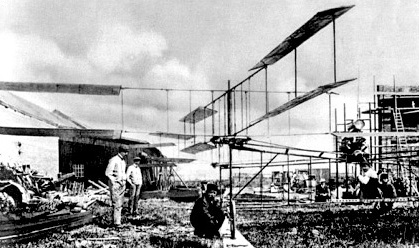
\includegraphics[width=\textwidth]{\DocRoot/images/breguet_gyro_1}
		\caption{Gyroplane No.1}
		\label{fig:Gyroplane No.1}
	\end{subfigure}%
	~ %add desired spacing between images, e. g. ~, \quad, \qquad, \hfill etc.
	%(or a blank line to force the subfigure onto a new line)
	\begin{subfigure}[b]{0.3\textwidth}
		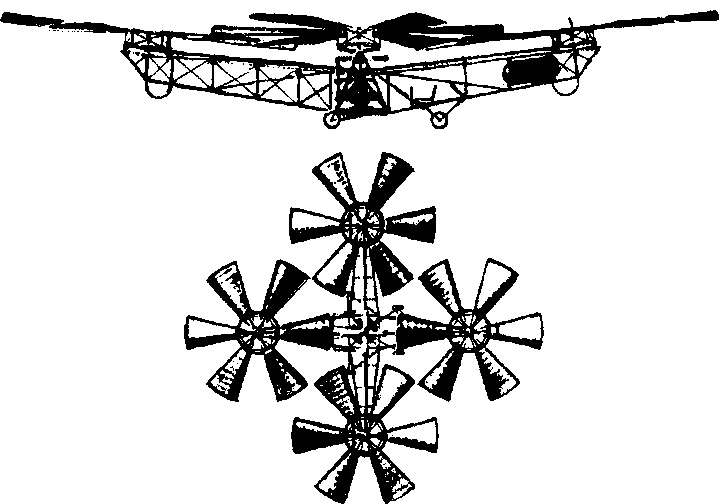
\includegraphics[width=\textwidth]{\DocRoot/images/bothezat_quad}
		\caption{Bothezat’s sketch}
		\label{fig:Bothezat’s sketch}
	\end{subfigure}
	~ %add desired spacing between images, e. g. ~, \quad, \qquad, \hfill etc.
	%(or a blank line to force the subfigure onto a new line)
	\begin{subfigure}[b]{0.3\textwidth}
		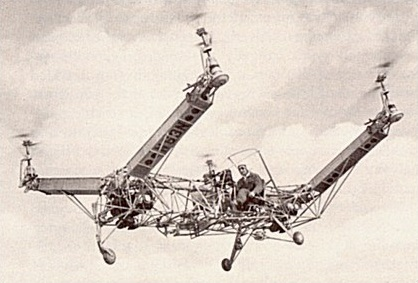
\includegraphics[width=\textwidth]{\DocRoot/images/convertawings}
		\caption{Convertawings Model A}
		\label{fig:Convertawings Model A}
	\end{subfigure}
	\caption{Development of the Quad-rotor concept \cite{Principles_of_helicopter_aerodynamics}}\label{fig:Development of the Quad-rotor concept}
\end{figure}


In  1921, the US Air Corps awarded a contract to Dr. George de Bothezat and Ivan Jerome to work on a vertical flight machine (see figure \ref{fig:Bothezat’s sketch}) \cite{Principles_of_helicopter_aerodynamics}. The result was a four six-bladed quad-rotor mounted at the ends of beams 20 metres in length arranged in a cross like structure. The craft overcame the stability problems present in quad-rotor built up until then by using two variable pitch controlled to ensure stability and control the craft. It was the first craft to prove that vertical flight  was possible despite it's limited reach of only 5 meters.

Due to stability problems the quad-rotor design   was abandoned in favour of research of the now traditional helicopter. It wasn't until 1956 that the concept of the quad-rotor was once again modernized with the “Convertawings Model A” \cite{Helicopters_and_autogiros(Convertawings_Model_A)} (see figure \ref{fig:Convertawings Model A}) whose development greatly improved the four rotor aircraft built by Oehmichen and Bothezat. With a simplified control system and greater power than its predecessors it was the first quad-rotor to fly successfully.


As a result of military interest the quad-rotor has been studied extensively as an alternative to traditional helicopters which were capable of carrying large payloads. The current and most widely known quad-rotor is the 2006 “Bell Boeing Quad Tilt-Rotor” (seen in figure \ref{fig:Bell Boeing Quad TiltRotor}), which was based on the two “Curtiss-Wright X-19” and “Bell X-22”  (see figures \ref{fig:Curtiss-Wright X-19.} and \ref{fig:Bell X-22.} respectively) which were two prototype quad-rotors built in the 1960's. The Bell Boeing Quad Tilt-Rotor was designed for military use to transport cargo of up to 9000kg to otherwise unreachable locations.   


\begin{figure}[h]
	\centering
	\begin{subfigure}[b]{0.35\textwidth}
		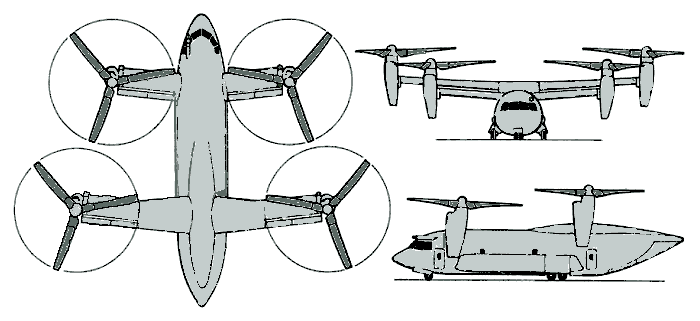
\includegraphics[width=4cm, height=3cm]{\DocRoot/images/QTRMV-44colour-1}
		\caption{Bell Boeing Quad Tilt-Rotor.}
		\label{fig:Bell Boeing Quad TiltRotor}
	\end{subfigure}%
	~ %add desired spacing between images, e. g. ~, \quad, \qquad, \hfill etc.
	%(or a blank line to force the subfigure onto a new line)
	\begin{subfigure}[b]{0.3\textwidth}
		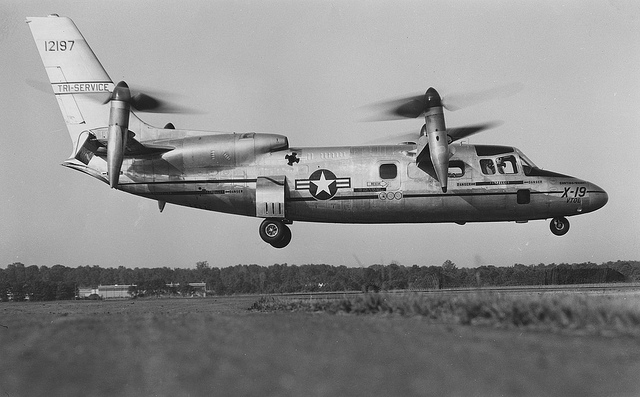
\includegraphics[width=4cm, height=3cm]{\DocRoot/images/6847501354_22de7e3548_z}
		\caption{Curtiss-Wright X-19.}
		\label{fig:Curtiss-Wright X-19.}
	\end{subfigure}
	~ %add desired spacing between images, e. g. ~, \quad, \qquad, \hfill etc.
	%(or a blank line to force the subfigure onto a new line)
	\begin{subfigure}[b]{0.3\textwidth}
		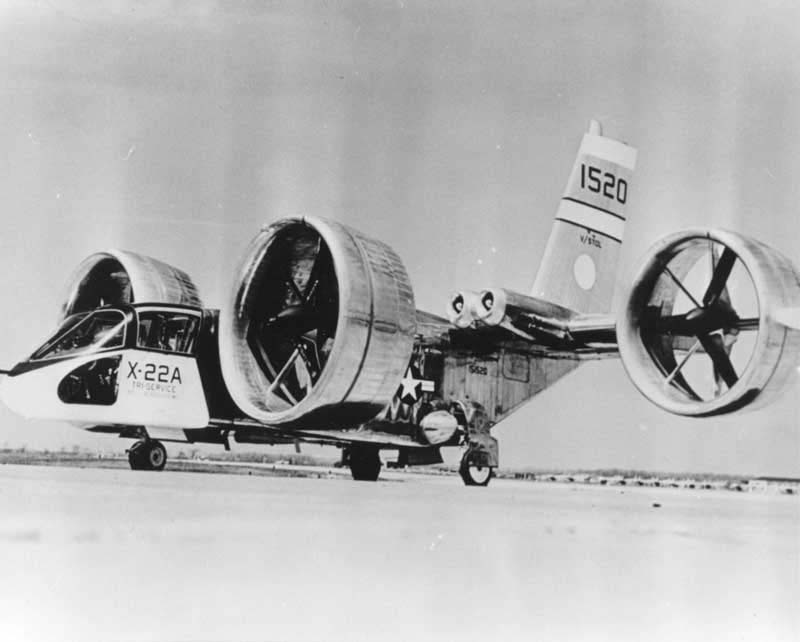
\includegraphics[width=4cm, height=3cm]{\DocRoot/images/X-22a_onground_bw}
		\caption{Bell X-22.}
		\label{fig:Bell X-22.}
	\end{subfigure}
	\caption{Further Development of the Quad-rotor Concept \cite{Principles_of_helicopter_aerodynamics}}\label{fig:Further Development of the Quadrotor Concept}
\end{figure}


Today, major breakthroughs in the concept of the quad-rotor have taken place in universities across the world. Examples of such break through are as follows; comparison of fixed-pitch and variable-pitch propeller based quad-rotors,  the development of  a robust controllers and test of a trajectory algorithm for variable-pitch aircrafts as seen in \cite{Variable_Pitch_Quadrotor_MIT, comparison_of_fixed_and_variable_pitch_actuators}. A paper written by a Czech researcher was found which develops an \gls{ekf} along with a \gls{lqr} based control system for a quad-rotor which was used to adequately control the system\cite{identification_and_Control_of_a_Quadrotor_(czech)}. In MIT a prototypes have been  developed  that are capable of exciting flips, and peak rotational rates exceeding $1600^{\circ}s^{-1}$ were accomplished using traditional fixed-pitch technology \cite{high_speed_quadrocopter_multi_flips}. Research groups have developed prototypes that can fly through windows and narrow gaps and perch on inverted surfaces \cite{Quad_fly_through_windows}. A group in ETH zurich are now combining the quad-rotor with traditional control problems such as the inverted pendulum \cite{flying_inverted_pendulum}. Other research personnel are currently focusing on mapping of areas using \gls{slam} and streaming the results to a a remote computer \cite{mapping_quad}. Note the improvement of the quad-rotors are not just limited to the military and academia; some hobbyists have developed \gls{rc} variable-pitch quad-rotors and have posted their findings on \gls{rc} forums and discussion boards \cite{misc_video}.

\begin{comment}
\section{Project Goals}
A benefit of doing a project in this area is the vast amount of information available about the subject of autonomous flight and the control/simulation of quad-rotors. 
The primary goal was to obtain a deeper understanding of control techniques, how one would implement them on a chip and improve programming skills in the process. The group's objective, was to control the quad-rotor in the hovering position in a certain location by using the supplied digital sensors \cite{accelerometer_datasheet,compass_datasheet,gyroscope_datasheet,rangefinder_datasheet,GPS_datasheet} and implement obstacle avoidance if possible. The main target was to obtain a complete and realistic control system for the quad-rotor with complete documentation so that the quad-rotor can be utilized in future projects/studies. 
\end{comment}


\chapter{Ethics}
Over the recent years quad-rotors have found use in many areas some of which have raised ethical issues. Currently, there are numerous ethical problems, primarily flying quad-rotors in urban areas. For most parts these devices have to abide by the same restrictions as \gls{rc} planes, i.e  to be flown below a maximum of 120 m, 150 m from other people and the operator has to maintain line of sight at all times \cite{quad_fly_ireland}. For research and commercial use written permission from the national aviation regulator is often required. Today, many hobbyists fly quad-rotors over urban areas: hobbyists feel they should be allowed to fly where they like (even with a camera on board) while the public want to maintain their privacy. 
Many quad-rotors sold to hobbyists some with holsters for a camera which are used to shoot video while in flight. The general public are very concerned about how this impacts privacy \cite{Consumer_drones}. Clear and well though out rules must be designed to deal with this issue. 
Due to this privacy issue there have been numerous bills passed in order to deal with this growing problem\cite{Quadcopters_Cameras}.



Certain companies have taken an interest in quad-rotors due to their capabilities to navigate urban areas with ease. Amazon and Google use programs based around quad-rotors delivering items \cite{amazon_drones}. Certain medical services are interested in drones to facilitate organ implants to remote locations as they can reach higher speeds, thus,  allowing more lives to be saved \cite{quad_ieee_med}. The concept of \gls{uav} is also being used to help herd cattle in remote locations in Australia  \cite{herding_video}. As a result of large companies investing in quad-rotors to such a large degree some people (couriers) are worried that they could loss their jobs to a quad-rotor. 

The military's interest in drones has driven the development of the quad-rotor to the level it is a today. The reasons the military have invested in such a platform such ass this must be considered when undertaking a dual use technology like this project  Since the conception of the quad-rotor the military have shown great interest because of its potential to reach difficult locations and their lifting capability, which can be seen from the development of the  “Bell Boeing Quad Tilt-Rotor”.  But more recently these drones have been used by the US and Israeli army for surveillance and there have been rumours/videos of quad-rotors being used as tactical weaponry \cite{quad-rotor_with_Machine_Gun, Armed_Quadrotors}. 

This potential dual use  means this project could be used to help or hinder the progress of mankind.
\chapter{Model Development}




\section{Quad-Rotor Dynamic} \label{sec: quad-model}


Helicopters and quad-rotors are complex flying machines due to their range of maneuverability \cite{Quadrotor_Helicopter_Flight_Dynamics_and_Control, Modelling_and_Control_of_a_Quad_Rotor_Robot}. Traditional helicopters are equipped with tail rotors to counteract the clockwise/anti-clockwise moments due to the motor. However, the \gls{uav} discussed in this report uses a different technique.

Quad-rotors are symmetrical vehicles with four equally sized rotors positioned at the end of their respective mountings. Quad-rotors use  multiple rotors so as to produce greater thrust and increase their maneuverability. Note that adjacent propeller blades are orientated opposite to each other. Thus if one set of rotors is spinning clockwise, then the two adjacent propellers have to spin counter-clockwise so that the torques produced by the propellers balance and cancel out if they all spin at the same rate

\begin{figure}[h]
	\centering
	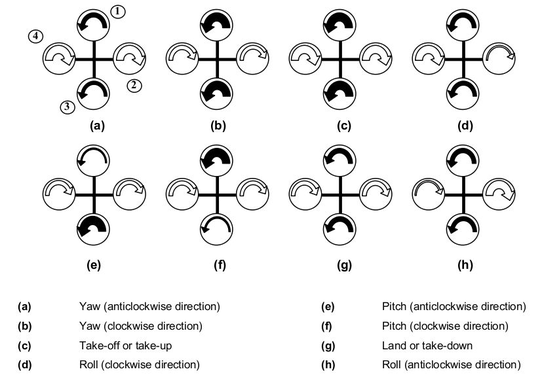
\includegraphics[width =0.7 \paperwidth]{\DocRoot/images/quad-rotor_control}
	\caption{Quad-Rotor Torque Pattern}
	\label{Fig:Quad-Rotor Torque Pattern}
\end{figure}







\subsection{Motor Model}\label{eq: quad rotor model}
For this project a first order linear model of the motor was used to relate motor speed to \gls{pwm}\footnote{ Note it is the duration of the high portion of the signal that sets the speed of the motor, not the percentage of the duty cycle which is high. This is different to traditional \gls{pwm} motor control. }. The first order modeled was used as it was difficult to find accurate values for the inductance and resistance of  the \gls{bldcm} that were used in this project.
\begin{align}
	\dot{\gls{rotationalvelocity}}=\frac{\gls{Motorcontant}\gls{PWMdutycycle}(t) - \gls{rotationalvelocity} }{\gls{timeconstants}}
\end{align}
Note the value for \gls{Motorcontant} was found from the experimental data and is 501.5 $\mathrm{Rad}s^{-2}$.

\subsection{Pitch}
Using Figure \ref{Fig:Quad-Rotor Torque Pattern} as a reference, the pitch of the quad-rotor can be defined using the following equations once one knows the difference in the moments about the pitch-axis.

\begin{equation}
	\tau_{\gls{pitch}} = \sum l \times F =\Delta M =  \gls{trustcoofmotor} \gls{lenghtfromcenterofmass}( \gls{rotationalvelocity}_1 ^2-\gls{rotationalvelocity}_3 ^2)
\end{equation}
Where  \gls{trustcoofmotor} is a constant linking angular acceleration to angular rotation, \gls{lenghtfromcenterofmass} is the distance from the point of rotation to the motors and \gls{rotationalvelocity} is the angular velocity of the motors.Thus, angular acceleration about the pitch axis can be defined as follows:-
\begin{align}
	\ddot{\gls{pitch}} & = \frac{\Delta M}{\gls{interiaofpitch}} =\frac{ \gls{trustcoofmotor} \gls{lenghtfromcenterofmass}( \gls{rotationalvelocity}_1 ^2-\gls{rotationalvelocity}_3 ^2)}{ \gls{interiaofpitch} }
	\label{eq: pitch model}
\end{align}
Where $\omega_1$ \& $\omega_3$ are the speed of motor one and three respectively. 
\subsection{Roll}
Similarly for roll, one can derive the following equation:-
\begin{align}
	\ddot{\gls{roll}} & = \frac{\Delta M}{\gls{interiaofroll}} =\frac{\gls{trustcoofmotor}\gls{lenghtfromcenterofmass}(\gls{rotationalvelocity}_2^2-\gls{rotationalvelocity}_4^2) }{\gls{interiaofroll}}
	\label{eq: roll model}
\end{align}
\subsection{Yaw}
Each of the spinning rotors creates a reaction torque which can cause the quad-rotor to spin about the z-axis which is positioned through the quad-rotor's centre of mass (assuming a uniform frame and equal distancing of the rotor from the centre of mass). Hence, the following equation for yaw can be defined:- 
\begin{align}
	\gls{reactiontorque} = \gls{inertiaofmotor}\dot{\gls{rotationalvelocity}}
\end{align}
The speed of the rotor and the drag coefficient also produce a reaction torque about the yaw axis which can be defined as follows :-
\begin{align}
	\gls{reactiontorquedrag} = \gls{dragcoofmotor} \gls{rotationalvelocity} ^2
\end{align}
Hence the rate of change of yaw is given by the following equation :-
\begin{align}
	\ddot{\gls{yaw}} & =\frac{\sum_{i=1}^{4} \gls{reactiontorque} + \sum_{i=1}^{4} \gls{reactiontorquedrag}  }{\gls{interiaofyaw}}
	\label{eq: yaw undefined}
\end{align}
Filling in for \gls{reactiontorque} and \gls{reactiontorquedrag}  into \eqref{eq: yaw undefined} one gets the following equation :-
\begin{align}
	\ddot{\gls{yaw}}=\frac{\gls{inertiaofmotor}(\dot{\gls{rotationalvelocity} _1}-\dot{\gls{rotationalvelocity} _2}+\dot{\gls{rotationalvelocity} _3}-\dot{\gls{rotationalvelocity}_4})+ \gls{dragcoofmotor} (\gls{rotationalvelocity}_1^2-\gls{rotationalvelocity} _2^2+\gls{rotationalvelocity} _3^2-\gls{rotationalvelocity} _4^2)}{\gls{interiaofyaw}} \label{d2ydt2}
\end{align}
Where, \gls{dragcoofmotor} is the drag coefficient of the propellers and \gls{inertiaofmotor} is the averaged inertia of the motors.  

\subsection{Movement in the Vertical \& Horizontal Directions}

To find the position of the quad-rotor in the vertical direction one can apply Newtons second law to find the following equation :-



\begin{align}
	\ddot{z} & = \left[\frac{\gls{trustcoofmotor}}{\gls{systemmass}}(\cos\gls{pitch} \cos\gls{roll})\sum_{i=1}^{4} \gls{rotationalvelocity} _i^2\right]   -g
\end{align}
Note the sum of the force in the vertical direction must be greater than the weight of the quad-rotor to ensure adequate lift.When the quad-rotor is pitched or rolled it must supply extra thrust to maintain its altitude \cite{identification_and_Control_of_a_Quadrotor_(lund)}.

If it is required to move in the horizontal plane the resultant trust of the quad-rotor has to be resolved as follows by means of Euler Rotations:- \label{Horizontal}
\begin{align}
	\ddot{x} & = \frac{\gls{trustcoofmotor}}{\gls{systemmass}}(\cos\gls{roll}\sin\gls{pitch}\cos\gls{yaw}+ \sin\gls{roll}\sin\gls{yaw} ) \sum_{i=1}^{4} \gls{rotationalvelocity} _i^2 \\
	\ddot{y} & = \frac{\gls{trustcoofmotor}}{\gls{systemmass}}(\cos\gls{roll}\sin\gls{pitch}\sin\gls{yaw} -\sin\gls{roll} \cos\gls{yaw})\sum_{i=1}^{4} \gls{rotationalvelocity} _i^2
\end{align}




\section{Kinematics and Dynamics Equations}

\subsection{Euler Angles} \label{sec: euler angles}
To describe the attitude and position of an object in free space (e.g an aircraft) a reference frame has to be attached to the object and then another can be attached to the earth, after which a relationship between the two coordinate systems can be defined. As the attitude of the device is expressed in the \gls{ned} frame and its angles \& velocity are measured by the \gls{9dof} in the Body Frame. Therefore it is necessary to be able to map from one frame to the other. 

Euler angles \footnote{Note in aviation these form of rotations are commonly refereed to as Tait–Bryan angles and are a sub-set of Euler angles} are not commutative and they must be applied in sequence to get the correct answer \cite[pg. 24]{Stanford_rotation_paper}. In this report the convention  \enquote{\textit{roll,pitch,yaw}}, denoted ($\gls{roll}, \gls{pitch}, \gls{yaw}$), which are rotations about the $(\bf x, y, z)$-axes respectively was adopted. As the accelerometer and gyroscope measurements take place in the Body Frame, the following mapping scheme was introduced so the orientation of the device could be defined in the same frame as the control. A rotation from the \gls{ned} frame to the Body Frame corresponds to a rotation about yaw {\bf R}$(\gls{yaw})^\intercal$, then about pitch {\bf R}$(\gls{pitch})^\intercal$ and finally about roll {\bf R}$(\gls{roll})^\intercal$, these equations are presented fully in \eqref{eq: rotation matrix in z direction1}.     



\begin{align}
	{\bf R}_1(\gls{roll})^\intercal  & \triangleq  \begin{bmatrix}
		1 & 0               & 0              \\
		0 & C_{\gls{roll}}  & S_{\gls{roll}} \\
		0 & -S_{\gls{roll}} & C_{\gls{roll}}
	\end{bmatrix},~
	{\bf R}_2(\gls{pitch})^\intercal & \triangleq  \begin{bmatrix}
		C_{\gls{pitch}} & 0 & -S_{\gls{pitch}} \\
		0               & 1 & 0                \\
		S_{\gls{pitch}} & 0 & C_{\gls{pitch}}
	\end{bmatrix},~
	{\bf R}_3(\gls{yaw})^\intercal   & \triangleq  \begin{bmatrix}
		C_{\gls{yaw}}   & S_{\gls{yaw}} & 0  \\
		- S_{\gls{yaw}} & C_{\gls{yaw}} & 0  \\
		0               & 0             & 1 
	\end{bmatrix}
	\label{eq: rotation matrix in z direction1}
\end{align}


Finally combining these three rotations presented in \eqref{eq: rotation matrix in z direction1} resulted in the following \footnote{For Mathematical ease $\sin(\alpha)$ was simplified to $S_{\alpha}$ and $\cos(\alpha)$ was simplified to $C_{\alpha}$. Note $\alpha$ is a place holder for the angle of interest.}:- 





\begin{equation}
	\gls{rotationmatrix} \triangleq {\bf R}(\gls{roll})^\intercal{\bf R}(\gls{pitch})^\intercal{\bf R}(\gls{yaw})^\intercal  \triangleq  \begin{bmatrix}
		C_{\gls{pitch}}	C_{\gls{yaw}}                                              & C_{\gls{pitch}} S_{\gls{yaw}}                                             & -S_{\gls{pitch}}               \\
		S_{\gls{roll}}S_{\gls{pitch}}C_{\gls{yaw}}  - C_{\gls{roll}}S_{\gls{yaw}} & S_{\gls{roll}}S_{\gls{pitch}}S_{\gls{yaw}}  + C_{\gls{roll}}C_{\gls{yaw}} & C_{\gls{pitch}}S_{\gls{roll}}  \\
		C_{\gls{roll}}S_{\gls{pitch}}C_{\gls{yaw}}  + S_{\gls{roll}}S_{\gls{yaw}} & C_{\gls{roll}}S_{\gls{pitch}}S_{\gls{yaw}}  - S_{\gls{roll}}C_{\gls{yaw}} & C_{\gls{pitch}}C_{\gls{roll}} 
	\end{bmatrix}
	\label{eq: rotation matrix1}
\end{equation}


{\bf where:-} \gls{rotationmatrix} corresponds to the rotation matrix which maps a vector in the \gls{ned} frame to the Body Frame. See Appendix \ref{chap: Rotation Matrix reation} for more information on rotation matrix and Euler Angles



\subsection{Singularities and Gimbal Lock}
Note if \gls{roll}, \gls{pitch} or \gls{yaw} = $\pi/2$ the rotation matrix presented in \eqref{eq: rotation matrix1} losses a degree of freedom. \eqref{eq: gimbel lock example} presents a rotation matrix which has loss a degree of freedom as \gls{pitch} was set equal to $\pi/2$. 

\begin{equation}
	\gls{rotationmatrix} =  \begin{bmatrix}
		0                                                          & 0                                                          & -1 \\
		S_{\gls{roll}}C_{\gls{yaw}}  - C_{\gls{roll}}S_{\gls{yaw}} & S_{\gls{roll}}S_{\gls{yaw}}  + C_{\gls{roll}}C_{\gls{yaw}} & 0  \\
		S_{\gls{roll}}S_{\gls{yaw}}  + C_{\gls{roll}}C_{\gls{yaw}} & C_{\gls{roll}}S_{\gls{yaw}}  - S_{\gls{roll}}C_{\gls{yaw}} & 0
	\end{bmatrix}
	=  \begin{bmatrix}
		0                          & 0                           & -1 \\
		S_{\gls{roll} - \gls{yaw}} & C_{\gls{roll} - \gls{yaw}}  & 0  \\
		C_{\gls{roll} - \gls{yaw}} & -S_{\gls{roll} - \gls{yaw}} & 0
	\end{bmatrix}
	\label{eq: gimbel lock example}
\end{equation}

In aviation this phenomenon is known as Gimbal Lock and corresponds to a reduction in degrees of freedom. As seen from \eqref{eq: gimbel lock example} a change in \gls{roll} and \gls{yaw} has the same effect, thus a degree of uncertainty has been introduced as one notation can represent two very different orientations. This is a problem when using Euler Angles, but as the quad-rotor was limited to $\pm 30^o$ on the \gls{pitch} and \gls{roll} axis this problem was avoided \footnote{Note the problem associated with a loss of freedom due to singularities can be alleviated by using quaternion, but they introduce their own problems as use dimensions to represent a point in free space.}. The limit on the pitch and roll was a result of the lifting power of the motors, once the angle becomes greater than $40 ^o$ the net upwards thrust is less than what is required to maintain the quad-rotor's altitude. 


\section{Inertial Measurement Unit} \label{sec:imu section for relation of stuff}
\subsection{Accelerometer model} \label{sec: acc model}
In order to estimate the attitude\footnote{Attitude are the set of (\gls{roll}, \gls{pitch}, \gls{yaw}) angles in the Body Frame with respect to the \gls{ned} frame.} of the quad-rotor an accelerometer was used to measure the direction of the gravity vector, g , from this the pitch and roll angles can be found. Let g be constant, pointing down along $z_n$ defined in the \gls{ned} frame with an intensity $g_0$ = 9.81 $\mathrm{m~s^{-2}}$ and let
$\bar{\bf a}^B$ denote the accelerometer measurement vector. The definition of $z_n$ can be seen in figure \ref{diag: diagram used to illistrate reference frames}. 

The accelerometer used in this project was an ADXL345, which uses the piezoelectric effect to an create electric signal due to accelerative forces acting on a micro-crystal structure inside the device, knowing this,the following equation was derived:-

\begin{equation}
	\bar{\bf a}^{B} = \gls{rotationmatrix}(g) - a^{B} +\mu_a+ \gls{accbais}  \label{eq:acc full equation1}
\end{equation}
Where: $\bar{\bf a}^{B}$is the sensor output in $\mathrm{m~s^{-2}}$;  g is the gravity vector in the \gls{ned} frame; $a^{B}$ is the acceleration of the quad-rotor; $\mu_a$ is the Gaussian noise component; \gls{accbais} is the constant bias of the accelerometer.


Note when the \gls{9dof} inertial measurement unit is placed at the center of mass \eqref{eq:acc full equation1} can  be shown to simplify to \eqref{eq:acc simplified equation1}. Note  \eqref{eq:acc simplified equation1} doesn't account for the fact that quad-rotor could be in free
fall in a horizontal position. If this occurred the output of the accelerometer would be 0. This could potentially be an issue.

Hence,in order to acquire attitude reads from the accelerometer a model was created that utilized the output vectors of the ADXL345 to estimate the attitude of the quad-rotor. \eqref{eq:acc simplified equation1} was used to estimate the attitude of the quad-rotor.


\begin{equation}
	\begin{bmatrix}
		\gls{ax} \\ \gls{ay} \\\gls{az}
	\end{bmatrix}
	= 
	g
	\begin{bmatrix}
		-S_{\gls{pitch}} \\ C_{\gls{pitch}}S_{\gls{roll}}\\C_{\gls{pitch}}C_{\gls{roll}} 
	\end{bmatrix}
	+
	\begin{bmatrix}
		\mu_{a-x} \\ \mu_{a-y}\\\mu_{a-z}
	\end{bmatrix}
	+
	\begin{bmatrix}
		\gls{accbaisx} \\ \gls{accbaisy}\\\gls{accbaisz}
	\end{bmatrix}
	\label{eq:acc simplified equation1}
\end{equation}





Now assuming that the bias and noise on the accelerometer is zero\footnote{These can be removed in code and by filtering methods respectively. These will be developed later in this report.} the orientation of the quad-rotor in the \gls{ned} frame can be calculated. Hence, \gls{roll} and \gls{pitch} can be defined as follows and can easily be shown to be correct by means of \eqref{eq:acc simplified equation1}:-

\begin{align}
	\begin{split}
		\gls{roll} &= \arctan\left(\frac{\gls{ay}}{\gls{az}}\right)\\
		\gls{pitch} &= \arctan \left(\frac{- \gls{ax}}{\sqrt{\gls{ay}^2+\gls{az}^2}}\right)
		\label{Eq: angles from acc1}
	\end{split}
\end{align}

\subsection{Gyroscope model} \label{sec: gyroscope sec}
A similar model was created for the gyroscope as the angular velocity measured by the gyroscope in the Body Frame doesn't correspond directly to the Euler angle rates $[\dot{\gls{roll}},\dot{\gls{pitch}},\dot{\gls{yaw}}]^\intercal$ . Instead the rate of change of angle can be defined with respect to the \gls{ned} frame as follows:-


\begin{equation}
	\begin{bmatrix}																
		\gls{wx} \\
		\gls{wy} \\
		\gls{wz}
	\end{bmatrix} =
	\begin{bmatrix}																
		1 & 0               & -S_{\gls{pitch}}              \\
		0 & C_{\gls{roll}}  & S_{\gls{roll}}C_{\gls{pitch}} \\
		0 & -S_{\gls{roll}} & C_{\gls{roll}}C_{\gls{pitch}}\end{bmatrix}
	\begin{bmatrix}																
		\dot{\gls{roll} } \\
		\dot{\gls{pitch}} \\
		\dot{\gls{yaw}}\end{bmatrix}
	\label{eq:gyroscope stuf}
\end{equation}

Now taking the in the inverse of \eqref{eq:gyroscope stuf} the following equation can be defined:-
\begin{equation}
	\begin{bmatrix}																
		\dot{\gls{roll} } \\
		\dot{\gls{pitch}} \\
		\dot{\gls{yaw}}
	\end{bmatrix}
	=
	\begin{bmatrix}																
		1 & S_{\gls{roll}}T_{\gls{pitch}}           & C_{\gls{roll}}T_{\gls{pitch}}          \\
		0 & C_{\gls{roll}}                          & -S_{\gls{roll}}                        \\
		0 & \frac{S_{\gls{roll}} }{C_{\gls{pitch}}} & \frac{C_{\gls{roll}}}{C_{\gls{pitch}}}
	\end{bmatrix}
	\begin{bmatrix}																
		\gls{wx} \\
		\gls{wy} \\
		\gls{wz}
	\end{bmatrix}
	\label{Eq: angleur velocity from gyro1}
\end{equation}

\subsection{Digital Compass model}

The magnetometer is a sensor designed to detect the magnetic North direction, written as {\bf  N\textsuperscript I}. By the definition of the reference frame and neglecting  magnetic inclination and magnetic declination, {\bf  N\textsuperscript I} = [0,1,0]\textsuperscript T.

A Honeywell HMC5883L was used in this project. The device works by measuring the change in resistance with a change in the applied magnetic field. The device can measure these change as it is made from strips of permalloy. As the device can measure the change in magnetic field, the orientation of the magnetic field can be estimated using the following:-  
\begin{equation}
	\bar{\bf N}^B = \gls{rotationmatrix}N^I + \mu_m + \gls{gyrobais} \nonumber
\end{equation}
{Where} $\bar{\bf N}^B$ is the sensor measurement which is subject to a Gaussain measurement noise, $\mu_m$, and a bias term, $b_m$.


Now, letting the magnetic field act completely through the $y$ component of \eqref{eq: rotation matrix1} so the quad-rotor will align up with the earths magnetic field along the $y$ axis. Hence, the following relation can be defined:-
\begin{equation}
	\begin{bmatrix}
		{\bf N}_x \\ {\bf  N}_y \\ {\bf  N}_z 
	\end{bmatrix}
	= 
	\begin{bmatrix}
		C_{\gls{pitch}}S_{\gls{yaw}}                                              \\ 
		S_{\gls{roll}}S_{\gls{pitch}}S_{\gls{yaw}}  + C_{\gls{roll}}C_{\gls{yaw}} \\
		C_{\gls{roll}}S_{\gls{pitch}}S_{\gls{yaw}} - S_{\gls{roll}}S_{\gls{yaw}}
	\end{bmatrix}
	+
	\begin{bmatrix}
		\mu_{m-x} \\ \mu_{m-y}\\\mu_{m-z}
	\end{bmatrix}
	+
	\begin{bmatrix}
		\gls{gyrobaisx} \\ \gls{gyrobaisy}\\\gls{gyrobaisz}
	\end{bmatrix}\label{eq: magnetometer read out}
\end{equation}

Thus, if both \gls{pitch} and \gls{roll} are known the compass readings can be compensated by means of the filtered \gls{pitch} and \gls{roll} data. This approach was possible as it was decided to filter the \gls{pitch} and \gls{roll} first and then compensate the \gls{yaw}. An approach similar to the one used on the accelerometer was done when defining \gls{yaw}, that is, the noise and bias were ignored as they can be filtered before \gls{yaw} is calculated. Hence, the following equation was derived so \gls{yaw} could be calculated:-

\begin{equation}
	\gls{yaw} = \arctan\left( \frac{ {\bf N}_x}{C_{\gls{roll}}C_{\gls{pitch}}{\bf N}_y - S_{\gls{roll}}C_{\gls{pitch}}{\bf N}_z - {\bf N}_x }\right)
	\label{eq:yaw com equation}
\end{equation}




\section{GPS Frame Conversion} \label{sec: gps part}
As one of the goals for this project was \gls{gps} navigation by means of way points, which is a method of relating latitude (\gls{latitude}) and longitude (\gls{longitude}) as illustrated in figure \ref{diag: diagram used to illistrate reference frames} was required. Thus, this section will deal with the mapping of \gls{latitude} and \gls{longitude} from a fixed frame attached to the earth (denoted \gls{ecef} to the \gls{ned} frame \cite{crassidis2006sigma}. 


If the quad-rotor required to move a certain distance in the $x, y$ or $z$ direction,this  distance has to be found in the \gls{ecef} frame first. The difference between the current location and the desired location must to be calculated. This difference can be found if the \gls{latitude} and \gls{longitude} of the destination is known and current \gls{latitude} and \gls{longitude} the quad-rotor is known. Once this is known, \eqref{Eq: xyz distance in circle coordinance1} can be used to find $xyz$ displacement in the \gls{ecef} and this is then mapped to the \gls{ned} frame using \eqref{Eq: ecef frame mapping1}. Note a similar approach can be used to control the velocity of the quad-rotor in the \gls{ned} frame.


\begin{align}
	\begin{split}
		N &= \frac{a}{\sqrt{1 - e^2\sin^2\gls{latitude}}}\\
		x&= (N+h)\cos(\gls{latitude})\cos(\gls{longitude})\\
		y &= (N+h)\cos(\gls{latitude})\sin(\gls{longitude})\\
		z &= [N(1-e^2)+h]\sin(\gls{latitude})
	\end{split}
	\label{Eq: xyz distance in circle coordinance1}
\end{align}


{

\begin{description}[itemsep=1mm]
	\item[{\bf Where:-}]
	\item[$h$:] is the height of the quad-rotor from the surface of the planet.
	\item[$a$:] is the equatorial radius of the earth and is equal to 6,378,137~$m$
	\item[$b$:] is the polar radius of the earth and is equal to 6,356,752.3142~$m$
	\item[$f$:] is flatting of the earth and is given by the following:- $f = (a-b)/a$
	\item[$e$:] is the eccentricity of the earth and is defined as follows:- $e= \sqrt{f(2-f) }$
\end{description}
}


In order to find out how far the quad-rotor has to go in order to reach the required position\footnote{And hence also control the quad-rotor} \eqref{Eq: xyz distance in circle coordinance1} has to be mapped using the following:-



\begin{equation}
	\begin{bmatrix}																
		\gls{north} \\
		\gls{east}  \\
		\gls{down}
	\end{bmatrix}
	\triangleq
	\begin{bmatrix}																
		-S_{\gls{latitude}o}C_{\gls{longitude}o} & -S_{\gls{latitude}o}S_{\gls{longitude}o} & C_{\gls{latitude}o}  \\
		-S_{\gls{longitude}o}                    & C_{\gls{longitude}o}                     & 0                    \\
		-C_{\gls{latitude}o}C_{\gls{longitude}o} & -C_{\gls{latitude}o}S_{\gls{longitude}o} & -S_{\gls{latitude}o}
	\end{bmatrix}
	\begin{bmatrix}																
		x_p - x_o \\
		y_p - y_o \\
		z_p - z_o 
	\end{bmatrix}
	\label{Eq: ecef frame mapping1}
\end{equation}

{\bf where:-} $(x_p, y_p, z_p)$ is the new point at which the quad-rotor has to move to and $(x_o, y_o, z_o)$ subscript is the current location of the quad-rotor. Similarly the velocity of the quad-rotor can using the heading and speed measurements that the \gls{gps} module. These measurements are given by the following equations:-

\begin{align}
	\begin{split}
		\mathrm{Speed} &= \sqrt{\dot{x_e}^2 +\dot{y_e}^2 }\\
		\mathrm{Heading} &= \textrm{arctan2}\left(\frac{\dot{x_e}}{\dot{y_e}}\right)
	\end{split}
\end{align}

Thus, the rate of change of position can also transformed by means of the following equations.

\begin{equation}
	\begin{bmatrix}																
		\dot{\gls{north}  } \\
		\dot{\gls{east}}    \\
		\dot{\gls{down}}
	\end{bmatrix}
	=
	\begin{bmatrix}																
		-S_{\gls{latitude}}C_{\gls{longitude}} & -S_{\gls{latitude}}S_{\gls{longitude}} & C_{\gls{latitude}}  \\
		-S_{\gls{longitude}}                   & C_{\gls{longitude}}                    & 0                   \\
		-C_{\gls{latitude}}C_{\gls{longitude}} & -C_{\gls{latitude}}S_{\gls{longitude}} & -S_{\gls{latitude}}
	\end{bmatrix}
	\begin{bmatrix}																
		\dot{x_e} \\
		\dot{y_e} \\
		\dot{z_e}
	\end{bmatrix}
	\label{Eq: ecef frame mapping velocity1}
\end{equation}




%Using a Taylor series approximation Equations \ref{Eq:x_lateral_lin} and \ref{Eq:y_lateral_lin} can be further linearised to Equations \ref{Eq:x_lateral_lin1} and \ref{Eq:y_lateral_lin2}
%\begin{align}
%\ddot{x} &= g\cdot \gls{pitch}\label{Eq:x_lateral_lin1}\\ 
%\ddot{y} &= -g\cdot \gls{roll}\label{Eq:y_lateral_lin2}
%\end{align}

{\bf where:-}
\begin{align}
	\begin{split}
		\dot{x_e} = \sqrt{\frac{(\mathrm{speed}^2)}{1 + \tan(\mathrm{heading})^2}}\\
		\dot{y_e} = \sqrt{(\mathrm{speed})^2 - \dot{x_e}^2}
	\end{split}
\end{align}

\tdplotsetmaincoords{75}{95}
%
\pgfmathsetmacro{\rvec}{.8}
\pgfmathsetmacro{\thetavec}{55}
\pgfmathsetmacro{\phivec}{35}

\pgfmathsetmacro{\rframe}{1.05}
\pgfmathsetmacro{\radiusphi}{0.4}
\pgfmathsetmacro{\framelengthz}{0.25}
\pgfmathsetmacro{\framelengthsxy}{0.18}
%
\definecolor{darkgreen}{rgb}{0.1,0.7,0.1}

\begin{figure}[h]
	\centering
	\resizebox{10.0cm}{10.0cm}{	\begin{tikzpicture}[scale=5,tdplot_main_coords]
			\tdplotsetcoord{P}{\rvec}{\thetavec}{\phivec}
			\tdplotsetcoord{Px}{0.55}{90}{\phivec}
			\coordinate (O) at (0,0,0);
			
			
			\draw[thick,->] (0,0,0) -- (1,0,0) node[anchor=north east]{$x_e$};
			\draw[thick,->] (0,0,0) -- (0,0.88,0) node[anchor=north west]{$y_e$};
			\draw[thick,->] (0,0,0) -- (0,0,0.88) node[anchor=south]{$z_e$};
			
			
			
			\draw[dashed,color=black] (O) -- (P);
			\draw[dashed, color=black, shorten >=-20pt ] (O) -- (Px);
			\tdplotdrawarc{(O)}{\radiusphi}{0}{\phivec}{anchor=north}{$\gls{longitude}$}
			\tdplotdrawarc[blue]{(O)}{0.8}{-90}{90}{}{}
			\tdplotdrawarc[dashed,blue]{(O)}{0.8}{90}{270}{}{}
			%
			\tdplotsetthetaplanecoords{\phivec}
			\tdplotdrawarc[tdplot_rotated_coords]{(0,0,0)}{\radiusphi}{\thetavec}%
			{90}{right}{$\gls{latitude}$}
			\tdplotdrawarc[tdplot_rotated_coords]{(0,0,0)}{0.8}
			{0}{90}{}{}
			%
			\tdplotsetthetaplanecoords{0}
			\tdplotdrawarc[tdplot_rotated_coords]{(0,0,0)}{0.8}{0}{90}{left}{\rotatebox[origin=cc]{85}{Prime Meridian}}
			%
			\tdplotsetthetaplanecoords{90}
			\tdplotdrawarc[tdplot_rotated_coords,blue]{(0,0,0)}{0.8}
			{0}{360}{}{}
			
			
			
			
			% NED Frame 
			\tdplotsetrotatedcoords{\phivec}{\thetavec}{0}
			\tdplotsetcoord{Q}{\rframe}{\thetavec}{\phivec}
			\tdplotsetrotatedcoordsorigin{(Q)}
			\draw[dashed,tdplot_rotated_coords,-,draw=green,fill=white] (-0.1,-0.1,0)
			-- (-0.1,0.1,0) -- (0.1,0.1,0)  -- (0.1,-0.1,0)  -- cycle  ;
			\draw[thick,tdplot_rotated_coords,->,black] (0,0,0)
			-- (-\framelengthsxy,0,0) node[thick,above]{$y_n$};
			\draw[thick,tdplot_rotated_coords,->,black] (0,0,0)
			-- (0,\framelengthsxy,0) node[thick,above]{$x_n$};
			\draw[thick,tdplot_rotated_coords,->,black] (0,0,0)
			-- (0,0,-\framelengthz) node[thick,right]{$z_n$};
		\end{tikzpicture}}
	\caption{Definitions of Various Reference Frames}
	\label{diag: diagram used to illistrate reference frames}
\end{figure}



\newpage
\section{Inertial Navigation System}
A system which uses Magnetometers, Accelerometers and Gyroscopes to estimate the attitude of a body is often referred to as a \gls{ins}. A method of estimating the attitude of quad-rotors has been the focus of substantial amount of research as the attitude data is required for autonomous flight. The attitude of the device dictates the direction in which the quad-rotor flies and thus is required for \gls{gps} navigation of a quad-rotor. 

As these sensors are not ideal it was  required to derive an accurate mathematical model of the quad-rotor and the sensors themselves.  As the accelerometer measurements contains linear, angular as well as acceleration due to gravity. This cannot be decoupled easily and hence requires a filter to remove these components. The gyroscope used was not ideal as the measurements tended to drift over time due to temperature. The magnetometer contained non-ideal components as any sources of ferromagnetic material placed close to the device will distort the magnetic field produced by the earth. A method to combine the accelerometer and gyroscope was required to give an adequate estimate of the orientation and was researched in detail. This estimate could then be used with a \gls{gps} device in order to control the quad-rotor remotely by means of \gls{gps} navigation. 



\subsection{Complementary Filter}
The Complementary Filter consists of two filters, a low-pass and a high-pass filter. The input to the low-pass filter is the accelerometer data, since at low accelerations, the accelerometer is considered to approximately measure only acceleration due to gravity. Hence, the orientation can be estimated. The input to the high-pass filter is the gyroscope data since the drift due to the gyroscope is low frequency. The algebraic sum of the outputs of the filters gives the estimate of the orientation.


\subsection{The Kalman Filter}
The Second method investigated was the Kalman Filter, which is much more difficult to design, but returns a more accurate result than the Complementer Filter. The Kalman Filter is based on the statistical properties of the noise in the sensor data, as well as the noise present in the model of the plant, which is assumed to be Gaussian in nature. Rudolf E. K\'alm\'an first presented it in 1960 when he published his famous paper describing a recursive solution to the discrete-data linear filtering problem \cite{kalman1960new}


But before such filtering methods are introduced, reasons must be presented for considering such advantaged filtering techniques. As can be seen from figure \ref{Fig:Cyan_unfilter_pitch_and_roll} the output from the sensors requires filtering of some form as the current noise is to great to control to allow adequate control of the quad-rotor. But if a low pass filter is used on the accelerometer the phase lag is too great to allow the required control, hence a estimator with less delay is required. Thus, the Complementary Filter and Kalman Filter were investigated.


\begin{figure}[h]
	\centering
	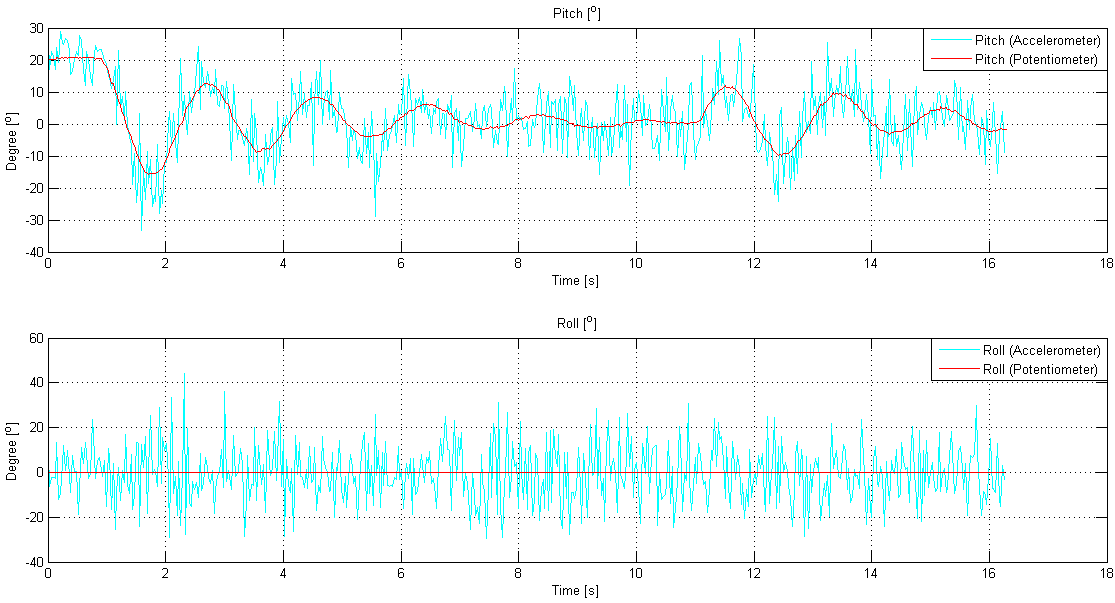
\includegraphics[width =0.7 \paperwidth]{\DocRoot/images/Cyan_unfilter_pitch_and_roll}
	\caption{Unfiltered Accelerometer Output vs Actual Angle}
	\label{Fig:Cyan_unfilter_pitch_and_roll}
\end{figure}

\chapter{The Complementary Filter}
Two different complementary filters were investigated and their responses were modeled in MatLab before they were tested on the Quad-Rotor. This chapter describes in detail these two complementary filters.

\section{ Complementary Filter}
The Complementary filter gets its name from the manner in which the high-pass and low-pass filters which make up the Complementary filter are chosen. Hence, a pair of filters are called complementary filters if their transfer functions sum to one at all frequencies in a complex sense, i.e. the phase is zero and the magnitude is one as seen in following:-

\begin{equation}
	G_1(s) + G_2(s) =1 \label{eq: bases of comp filter1}
\end{equation}



Figure \ref{fig: Block Diagram of First Order Complementary Filter} is a block diagram representation of a first order complementary filter. As can be seen from the figure, the accelerometer data is low pass filtered while the gyroscope data is high pass filtered. The filters used in this report are augmented forms of the filters presented in \cite{sprague2001design,comp_filter_mit}. The first filter that was investigated first and is depicted in figure \ref{fig: Block Diagram of First Order Complementary Filter}.


\tikzset{%
block/.style    = {draw, thick, rectangle, minimum height = 3em,minimum width = 3em},
input/.style    = {coordinate}, % Input
output/.style   = {coordinate} % Output
block/.style    = {draw, thick, rectangle, minimum height = 3em,minimum width = 3em},
gain/.style     = {draw, thick, isosceles triangle, minimum height = 2em,
		isosceles triangle apex angle=60},
port/.style     = {inner sep=0pt, font=\tiny},
sum/.style n args = {4}{draw, circle, node distance = 2cm, minimum size=5mm, alias=sum,
		append after command={
				node at (sum.north) [port, below=1pt] {$#1$}
				node at (sum.west) [port, right=1pt] {$#2$}
				node at (sum.south) [port, above=1pt] {$#3$}
				node at (sum.east) [port, left=1pt] {$#4$}
			},
	}, % Adder
joint/.style    = {circle, draw, fill, inner sep=0pt, minimum size=2pt},
input/.style    = {coordinate}, % Input
output/.style   = {coordinate} % Output
}
% Defining string as labels of certain blocks.
\newcommand{\suma}{\Large$+$}
\newcommand{\inte}{$\displaystyle \int$}
\newcommand{\derv}{\huge$\frac{d}{dt}$}


\begin{figure}[h]
	\centering
	\begin{tikzpicture}[auto, thick, node distance=2cm, >=triangle 45]
		\draw
		% Drawing the blocks of first filter :
		
		node at (0,0) [input,name=input1,thick,above]{}
		node at (4,0)[block] (lpf) {\Large $\frac{1}{1+\tau s}$}
		node at (0,-2) [name=input2] {}
		node at (6,-2) [block](inte1) {\inte}
		node at (4,-2)[block] (hpf) {\Large $\frac{s}{1+\tau s}$}
		node at (8,-1)[sum={+}{}{+}{}] (suma1) {}
		node at (12,-1) [name=out] {};
		% Commands \draw with options like [->] must be written individually
		\draw[->](input1) -- node {$\text{Accel output}~(\gls{accdata})$} (lpf);
		\draw[->](input2) -- node {$\text{Gyro output}~(\gls{gyrodata})$}(hpf);
		\draw[->](hpf) -- node {}(inte1);
		\draw[->](inte1) -| node {}(suma1);         %note the -| does the right angle
		\draw[->](lpf) -| node {}(suma1);
		\draw[->](suma1) -- node {$\text{Filtered Data}~(\gls{filterdata})$}(out);
	\end{tikzpicture}
	\caption{Block Diagram of First Order Complementary Filter}
	\label{fig: Block Diagram of First Order Complementary Filter}
\end{figure}







\newpage
\subsection{First Order Complementary Filter}
The first order complementary filter presented in \cite{sprague2001design} is best represented by \eqref{eq: filter order filter1}\footnote{Note it is assumed that the sensors have ideal transfer functions i.e $H_a(s) = H_g(s) = 1$, where $H_a(s)~\&~H_g(s)$ are the transfer functions of the accelerometer and the gyroscope respectively}. As can be seen from \eqref{eq: filter order filter1} there is only one tuning parameter ($\tau$), meaning the filter is easy to design. Therefore there is a trade off between ease of use and versatility with the first order filter. 


The first order filter gave adequate results, a second order complementary filter will also be presented later which has two tuning parameters, which is a more versatile version of the Complementary Filter.


\begin{equation}
	\gls{filterdata} = \underbrace{\frac{1}{1 + \tau s}}_{\text{$G_1(s)$}}\gls{accdata} + \underbrace{\frac{\tau s}{1 + \tau s}}_{\text{$G_2(s)$}}\frac{1}{s}\gls{gyrodata}
	\label{eq: filter order filter1}
\end{equation}
As can be seen from Figure \ref{Fig:bode first order com} the filters presented in \eqref{eq: filter order filter1} are indeed complementary.   

\begin{figure}[h]
	\centering
	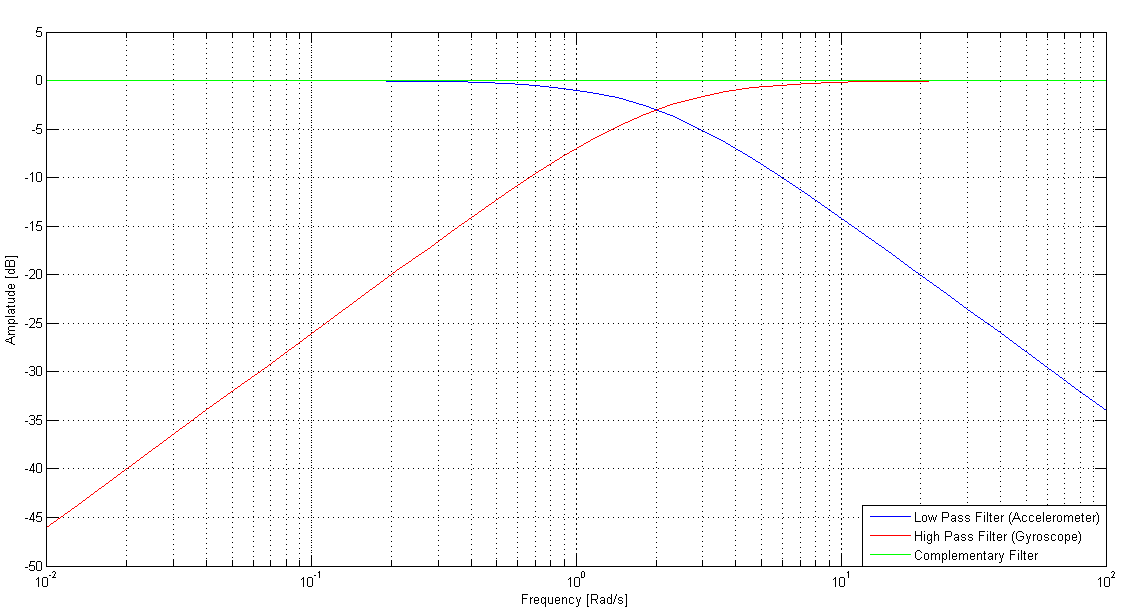
\includegraphics[width =0.7 \paperwidth]{\DocRoot/images/first_order_bode_plot}
	\caption{Bode plot of first order complementary filter}
	\label{Fig:bode first order com}
\end{figure}


Note as the orientation required for the control of the quad-rotor is in the \gls{ned} frame and as the sensor readings were in the \gls{bf} frame, a mapping was required to ensure the correct angles. These mappings which were presented in \eqref{Eq: angles from acc1}, \eqref{Eq: angleur velocity from gyro1} and\eqref{eq: filter order filter1}. These mappings allowed 
the high frequency components to be filtered so that an adequate estimation of the orientation could be achieved by means of a high-pass on gyroscope data:-
\begin{align}
	\dot{\gls{roll}}_{hp}  & =   \gls{wx} + S_{\gls{roll}}T_{\gls{pitch}}\gls{wy} + C_{\gls{roll}}T_{\gls{pitch}}\gls{wz}   - \frac{\gls{roll}_{hp}}{\tau} \\
	\dot{\gls{pitch}}_{hp} & =  C_{\gls{roll}}\gls{wy} - S_{\gls{roll}}\gls{wz} - \frac{\gls{pitch}_{hp}}{\tau}
\end{align}

By a similar mapping system the following low frequency components can be derived by means of a low-pass filter on the accelerometer:-

\begin{align}
	\dot{\gls{roll}}_{lp}  & =   \frac{1}{\tau}\left[\arctan\left(\frac{\gls{ay}}{\gls{ay}}\right) - \gls{roll}_{lp}\right]                      \\
	\dot{\gls{pitch}}_{lp} & =  \frac{1}{\tau}\left[\arctan\left(\frac{-\gls{ax}}{\sqrt{\gls{ay}^2+\gls{az}^2}}\right) - \gls{pitch}_{lp}\right]
\end{align}

\subsection{Difference Equations for first order filter}
Equation \ref{eq: filter order filter1} was emulated into the digital domain using Tustin's approximation to integration. Tustin's method was chosen as it ensures a stable mapping into the discrete domain (maps to inside the unit circle) if the continues function is stable.
\begin{equation}
	\begin{split}
		\gls{filterdata} [k] = \frac{1}{\gls{ts} + 2\tau}(\gls{ts} ( \gls{accdata} [k] + \gls{accdata} [k-1]  +  \tau(\gls{gyrodata} [k] + &\gls{gyrodata} [k-1])) \\ &-(\gls{ts} -2\tau)\gls{filterdata} [k-1] ) \label{eq: diff equation for the first order comp filter}
	\end{split}
\end{equation}


Equation \ref{eq: diff equation for the first order comp filter} was implemented on the micro-controller without the frame adjustments stated in \eqref{eq:acc simplified equation1} and \eqref{Eq: angleur velocity from gyro1}. These reductions were possible as the pitch (\gls{pitch}) and roll (\gls{roll}) angles were limited to $\pm 30^o$, these limitations allowed the trigonometric functions presented in \eqref{Eq: angleur velocity from gyro1} and \eqref{eq:acc simplified equation1} to be modeled as unity and \gls{pitch} or \gls{roll} for the $cos$ and $sin$ functions respectively. This was employed to reduce the sampling time of the critical control loops and can be easily added again if a faster micro-controller with a hardware \gls{fpu} \footnote{A micro-controller that has these requirements is the \textit{Tiva-C LaunchPad} which features a ARM Cortex-M4F which has a hardware \gls{fpu}} is used for the project in the future.  

The first order filter shown above was implemented both in Simulink and on the micro-controller along with the attitude controller. The filter was tuned in a similar method presented in algorithm \ref{Alg: auto tune of comp filter1} where the phase delay and \gls{rmse} weightings were adjusted until an adequate result was reached. Figure \ref{fig first order comp time and freq responce} compares the estimated pitch angle to the actual value. The results are adequate, but the gyroscope drift has not been fully eliminated and so another method of estimating the attitude of the quad-rotor was investigated. It was first decided to investigate a second order Complementary Filter. 

\begin{figure}[h]
	\centering
	\begin{subfigure}{0.32\textwidth}
		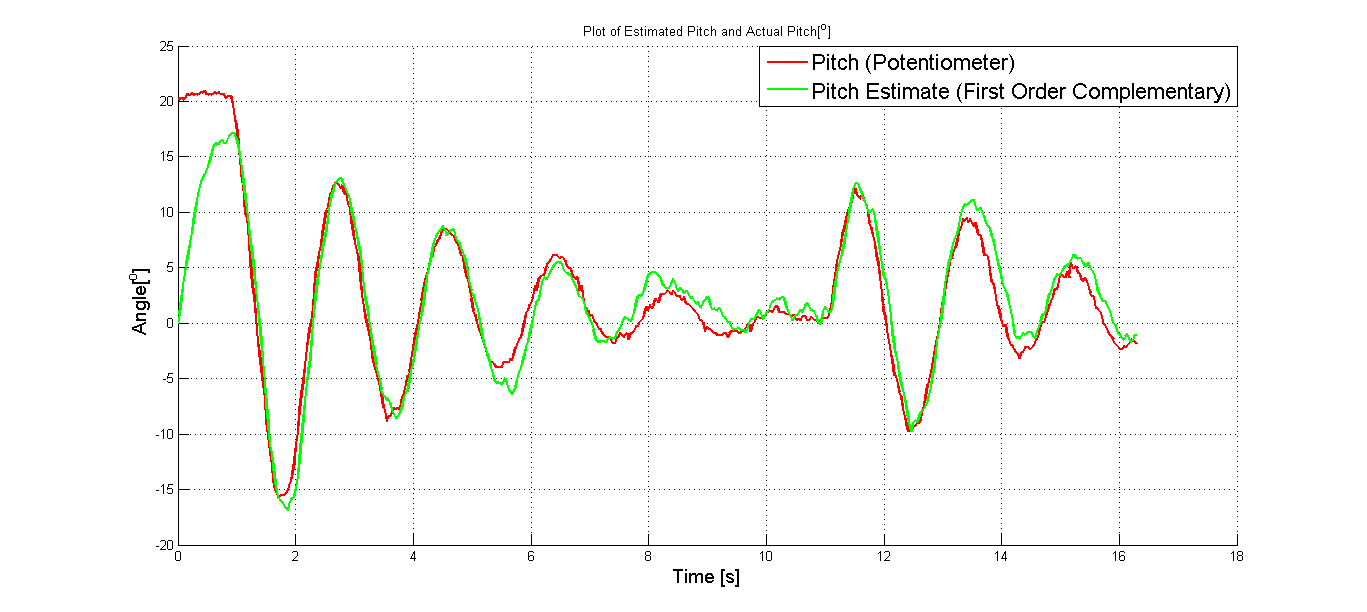
\includegraphics[width =0.36\paperwidth]{\DocRoot/images/comp_first_order_time}
		\caption{Time domain response of a first order Complementary Filter}
		\label{fg: Time domain comparison responce of the first order comp filter}
	\end{subfigure}%
	\hspace{3cm}
	\begin{subfigure}{0.32\textwidth}
		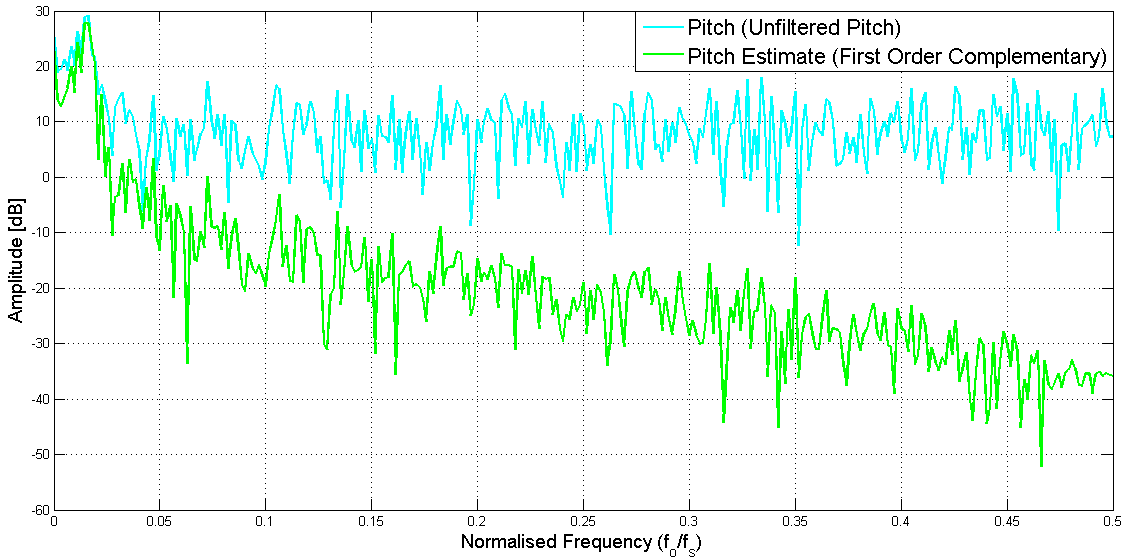
\includegraphics[width =0.36\paperwidth]{\DocRoot/images/comp_first_order_freq}
		\caption{Frequency domain response of a first order Complementary Filter}
		\label{fg: Frequency domain responce of the first order comp filter}
	\end{subfigure}
	
	\caption{Response of a first order complementary filter for $\tau = 0.5$ and ${\gls{ts}} = 30~\mathrm{ms}$ }
	\label{fig first order comp time and freq responce}
\end{figure}

\subsection{Second Order Complementary Filter}
As the drift on the gyroscope was still present after implementing the first order complementary filter on the micro-controller it was decided to implement a second order complementary filter similar to the one researched by Mahony \& Madgwick \cite{comp_filter_mit}. The filter presented in this section has two tuning parameters $K_p~\&~K_i$, this means that this filter is more versatile than the first order complementary filter which has only one tunning parameter $\tau$.



\begin{figure}[h]
	\begin{subfigure}[b]{0.32\textwidth}
		\resizebox{7.5cm}{3cm}
		{\begin{tikzpicture}[auto, thick, node distance=2cm, >=triangle 45]
				\draw
				% Drawing the blocks of first filter :	
				node at (0,0) [input,name=input1,thick,above]{}
				node at (3,0)[block] (lpf) {\Large $\frac{K_i + K_ps}{K_i +K_ps + s^2}$}
				node at (0,-2) [name=input2] {}
				node at (5.5,-2) [block](inte1) {\inte}
				node at (3,-2)[block] (hpf) {\Large $\frac{s^2}{K_i + K_ps +s^2}$}
				node at (7,-1)[sum={+}{}{+}{}] (suma1) {}
				node at (9,-1) [name=out] {};
				% Commands \draw with options like [->] must be written individually
				\draw[->](input1) -- node {$\gls{accdata}$} (lpf);
				\draw[->](input2) -- node {$\gls{gyrodata}$}(hpf);
				\draw[->](hpf) -- node {}(inte1);
				\draw[->](inte1) -| node {}(suma1);         %note the -| does the right angle
				\draw[->](lpf) -| node {}(suma1);
				\draw[->](suma1) -- node {$\gls{filterdata}$}(out);
			\end{tikzpicture}}
		\vspace{0.2cm}
		\caption{Block Diagram of Second Order Complementary Filter}
		\label{fig: Block Diagram of Second Order Complementary Filter}
	\end{subfigure}%
	\hspace{3cm}
	\begin{subfigure}[b]{0.32\textwidth}
		\resizebox{7.5cm}{3.5cm}{\begin{tikzpicture}[auto, thick, node distance=2cm, >=triangle 45]
				\draw
				% Drawing the blocks of first filter :
				node at (-0.3,0)     {$\gls{accdata}$}
				node at (0,0)      [input,name=input1,thick,above]{}
				node at (-0.3,-2.5)  {$\gls{gyrodata}$}
				node at (0,-2.5)   [input,name=input2,thick,above]{}
				
				node at (1,0)[sum={}{-}{+}{}] (sum1) {}
				node at (2,0) [joint] (joint1) {}
				node at (4,0) [block](inte1) {\inte}
				node at (6,0) [gain](ki){$K_i$}
				node at (4,2) [gain](kp){$K_p$}
				node at (7.5,0)[sum={+}{+}{}{}] (sum2) {}
				node at (8.5,0)[sum={}{-}{+}{}] (sum3) {}
				node at (10,0) [block](inte2) {\inte}
				node at (11,0) [joint] (joint2) {}
				node at (11.5,0) (out) {}
				node at (11.7,0)  {$\gls{filterdata}$};
				
				% Commands \draw with options like [->] must be written individually
				\draw[->](input1) -- node {}(sum1);
				\draw[->](sum1) -- node {} (inte1);
				\draw[->](joint1) |- node {} (kp);
				\draw[->](inte1) -- node {} (ki);
				\draw[->](ki) -- node {} (sum2);
				\draw[->](kp) -| node {} (sum2);
				\draw[->](input2) -| node {} (sum3);
				\draw[->](sum2) -- node {} (sum3);
				\draw[->](sum3) -- node {} (inte2);
				\draw[->](inte2) -- node {} (out);
				\draw(joint2) -- ++(0,-1.5) [->] -| node {} (sum1);
			\end{tikzpicture}}
		\caption{Feedback Block Diagram of Second Order Complementary Filter}
		\label{fig:Feedback Block Diagram of Second Order Complementary Filter2}
	\end{subfigure}
	\caption{Second Order Complementary Filter Block Diagrams}
	\label{fig: second order comp filter}
\end{figure}


The second order complementary filter described in figure \ref{fig: second order comp filter} can be defined over all frequencies by \eqref{eq: second order filter1}:-


\begin{equation}
	\gls{filterdata}=\underbrace{ {\frac{K_i + K_p s}{K_i + K_p s + s^2}}}_{\text{$G_1(s)$}}\gls{accdata} + \underbrace{\frac{s^2}{K_i+K_p s + s^2}}_{\text{$G_2(s)$}}\frac{1}{s}\gls{gyrodata}
	\label{eq: second order filter1}
\end{equation}

As can be seen from Figure \ref{Fig:bode sec order com} the filters presented in \eqref{eq: second order filter1} are complementary.   


\begin{figure}[h]
	\centering
	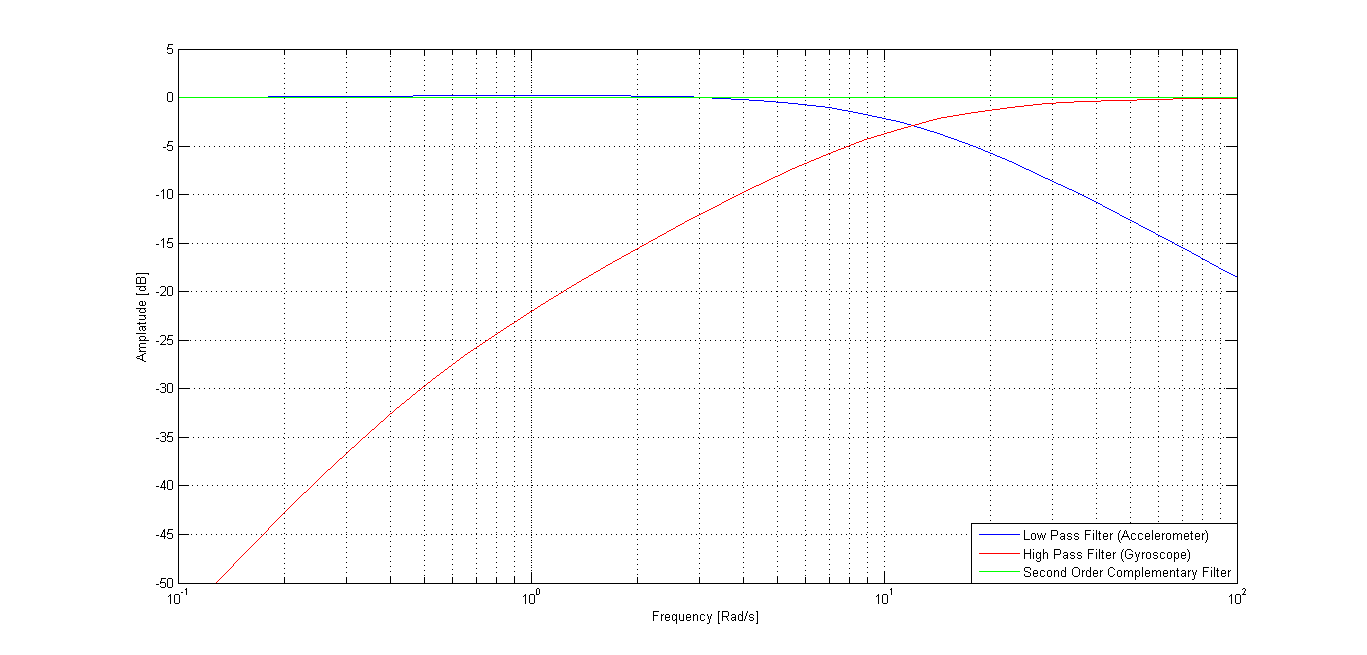
\includegraphics[width =0.8 \paperwidth]{\DocRoot/images/sec_order_bode_plot}
	\caption{Bode plot of a common second order complementary filter}
	\label{Fig:bode sec order com}
\end{figure}

Obviously, and not unexpectedly, this complementary filter is made from $2^{\mathrm{nd}}$ order filters. Note that the filter acting on the acceleration data actually consists of a low-pass plus a band-pass filter.

This result has interesting consequences. As the filters are $2^{\mathrm{nd}}$ order, the frequency response of the acceleration and gyroscope filters are characterized by the resonance frequency and damping factor

\begin{equation}
	\omega_0 = \sqrt{K_i}~~~~~~~ \xi = \frac{K_p}{2\sqrt{K_i}}
	\label{eq: second order comp filter ki and kp}
\end{equation}


The damping factor determines the overshoot at the resonance frequency. For manual tuning of this filter a flat frequency response can be achieved by setting $\xi \geq 1$ in \eqref{eq: second order comp filter ki and kp}. After doing this, one will get the following tuning criteria. 

\begin{equation}
	K_i \leq \frac{1}{4}K_p^2
\end{equation}
The results of this type of tuning can be seen in Figure \ref{fig sec order comp time and freq responce} and estimated the orientation of the quad-rotor to a certain degree, but as a whole was unsatisfactory. As a result two other methods of auto-tuning the filter were investigated, one which used a least squares and another which used a grid search. Before a grid based tuning approach could be implemented a discrete time version of the filter had to be created. 

Thus, to model the filter in MatLab $G_1(s)$ and $G_2(s)$ were arranged as follows:-
\begin{align}
	\chi_{hp} & = \frac{1}{s}\left[\gls{gyrodata} - \chi_{hp}\left({\frac{K_i}{s} + K_p}\right)\right] \label{Eq: second order comp high pass second1} \\
	\chi_{lp} & = \frac{1}{s}\left[(\gls{accdata} - \chi_{lp})\left({\frac{K_i}{s} + K_p}\right)\right] \label{Eq: second order comp low pass second1}
\end{align}


Note \eqref{Eq: second order comp high pass second1} and \eqref{Eq: second order comp low pass second1} can be combined to yield the following filter (as $\chi_{hp} + \chi_{lp} =  \gls{filterdata} $), which can also be modeled in MatLab.

\begin{equation}
	\gls{filterdata}  = \frac{1}{s}\left[\gls{gyrodata} +\left({\frac{K_i}{s} + K_p}\right)(\gls{filterdata}   - \gls{accdata})\right] \label{eq: comp filter equation used to tune comp filter1}
\end{equation}

\begin{figure}[h]
	\centering
	\begin{subfigure}{0.32\textwidth}
		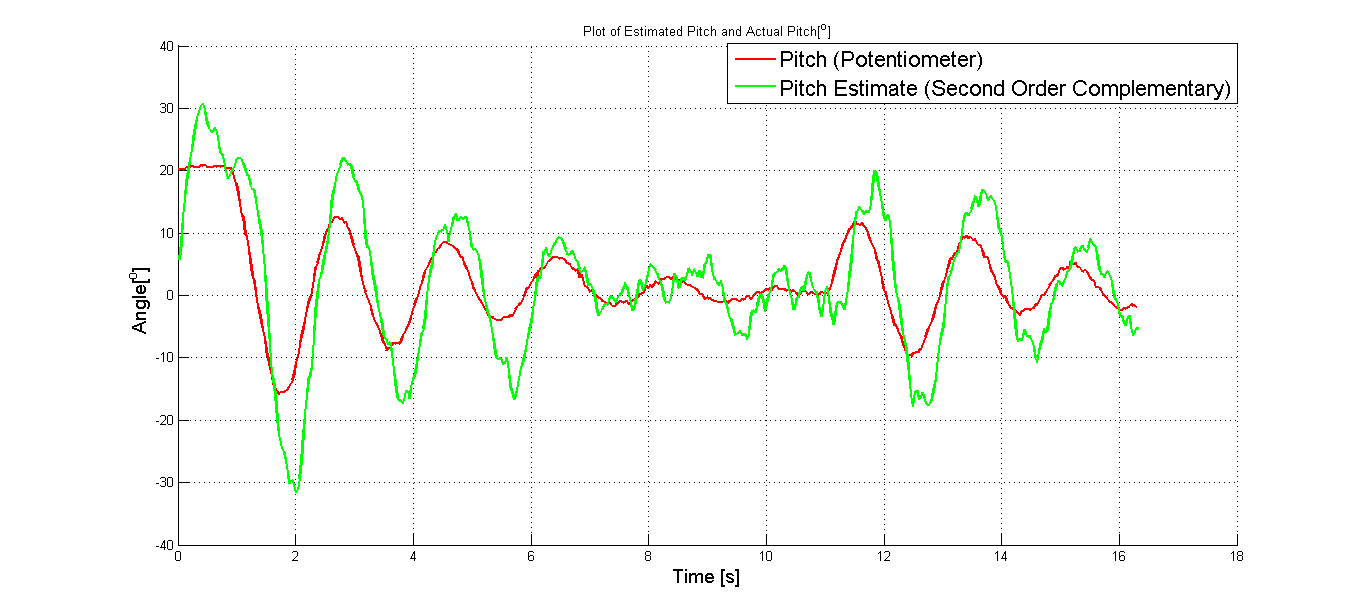
\includegraphics[width =0.38\paperwidth]{\DocRoot/images/comp_sec_time_man}
		\caption{Time domain response of a Second order Complementary Filter}
		\label{fg: Time domain comparison responce of the sec order comp filter}
	\end{subfigure}%
	\hspace{3cm}
	\begin{subfigure}{0.32\textwidth}
		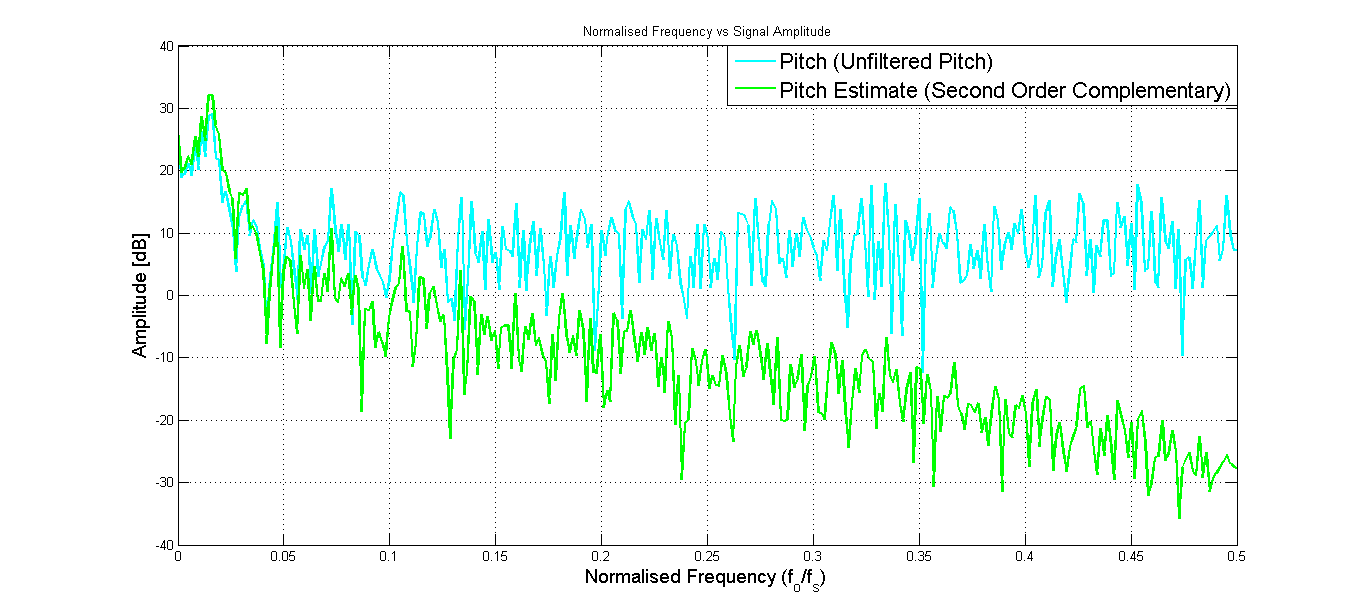
\includegraphics[width =0.38\paperwidth]{\DocRoot/images/comp_sec_fre_man}
		\caption{Frequency domain response of a Second order Complementary Filter}
		\label{fg: Frequency domain responce of the sec order comp filter}
	\end{subfigure}
	
	\caption{Response of a Second order complementary filter for $K_i = 25$, $K_p = 7$ and ${\gls{ts}} = 30~\mathrm{ms}$ }
	\label{fig sec order comp time and freq responce}
\end{figure}

\newpage
\subsection{Difference Equations for second order filter}
In order to implement the second order complementary filter on a micro-controller \eqref{Eq: second order comp high pass second1}and \eqref{Eq: second order comp low pass second1} were emulated into the digital domain using Tustin's method, which yielded the following equations:-
\begin{align}
	\chi_{hp}[k] & = \frac{1}{\eta + 4}\left(2\gls{ts} ( \gls{gyrodata} [k] - \gls{gyrodata} [k -2] ) - (\Gamma + 4)\chi_{hp}[k-2] - (\xi - 8)\chi_{hp}[k-1] \right) \label{Eq: second order comp high pass second difference eq1}                       \\
	\chi_{lp}[k] & = \frac{1}{\eta +4}\left(\Gamma \gls{accdata} [k-2] + \xi \gls{accdata} [k-1] + \eta \gls{accdata} [k] - (\Gamma + 4)\chi_{lp}[k-2] - (\xi - 8) \chi_{lp}[k - 1] \right) \label{Eq: second order comp low pass second difference eq1}
\end{align}


where:-

\begin{equation*}
	\eta = K_i\gls{ts}^2 + 2K_p\gls{ts};~~~ \Gamma = K_i\gls{ts}^2 - 2 K_p\gls{ts};~~~ \xi = 2K_i\gls{ts}^2
\end{equation*}

Before auto-tuning of the filter was implemented \eqref{Eq: second order comp high pass second difference eq1} and \eqref{Eq: second order comp low pass second difference eq1} where combined to give \eqref{Eq: full dfference equation for the second order filter1}. This was the equation that was used to tune the filter. Note \eqref{eq: comp filter equation used to tune comp filter1} could also be used to tune the filter, but when the filter is emulated there are distortions introduced by the emulation process.

\begin{multline}
	\gls{filterdata} [k] = \frac{1}{\eta +4}(\Gamma \gls{accdata} [k-2] + \xi \gls{accdata} [k-1] + \eta \gls{accdata} [k] + 2\gls{ts} ( \gls{gyrodata} [k] \\
	- \gls{gyrodata} [k -2] )   - (\Gamma + 4)\gls{filterdata} [k-2] - (\xi - 8) \gls{filterdata} [k - 1] ) \label{Eq: full dfference equation for the second order filter1}
\end{multline}

\section{Tuning of the Complementary Filter using Least Squares }
As a manual approach to tuning the second order filter yielded inadequate results, other methods of tuning the filter were investigated. One of the more useful approaches to tuning the filter was the least squares approach. Using \eqref{eq: comp filter equation used to tune comp filter1} one can tune the filter in the continuous domain and then emulate it across. This can be done by making the following assumption:-
\begin{equation}
	\gls{filterdata} = \gls{potangle}
\end{equation}
Where \gls{potangle} is the angle of the system as given by the potentiometer. In order to accomplish this  access to the rate of change of potentiometer angle as denoted as $\dot{\gls{potangle}}$. Hence, a method of tuning the filter as follows:-



\begin{align}
	\begin{split}
		\gls{potangle} &= \frac{1}{s}\left[ \gls{gyrodata} -\left(K_p + \frac{K_i}{s}\right) (\gls{potangle} - \gls{accdata})\right]\\
		\dot{\gls{potangle} }&= \left[ \gls{gyrodata} -\left(K_p + \frac{K_i}{s}\right) (\gls{potangle} - \gls{accdata})\right]\\
		\underbrace{\dot{\gls{potangle} } - \gls{gyrodata}}_{\text{$B_f$}}& = \underbrace{\left[(\gls{gyrodata} - \gls{potangle} ) + \frac{(\gls{gyrodata} - \gls{potangle} )}{s} \right] }_{\text{$A_f$}} \left[\begin{array}{c} K_p\\ K_i\end{array}\right] \label{eq: placer for leasr square eqaution1}
	\end{split}
\end{align}

Thus, using the equation developed in \eqref{eq: placer for leasr square eqaution1} one can tune a continuous time complementary filter of this form using the following:- 
\begin{equation}
	\left[\begin{array}{c} K_p\\ K_i\end{array}\right] = (A_f^\intercal A_f)^{-1}A_f^\intercal B_f \label{eq: tuning of complmentry filter in continues time least squares1}
\end{equation}

Note the method of tuning the filter as shown in \eqref{eq: tuning of complmentry filter in continues time least squares1} was done without a $\dot{\gls{potangle}}$ term. Instead a value was set for $(\gls{gyrodata} - \dot{\gls{potangle})}$ which was a valid approximation as the output of the gyroscope was low pass filtered on-chip with a first order filter which has a cutoff frequency of 100 \textit{Hz}. The results of this tuning method can be seen in Figure \ref{fig sec order comp time and freq responce least}


\begin{figure}[h]
	\centering
	\begin{subfigure}{0.32\textwidth}
		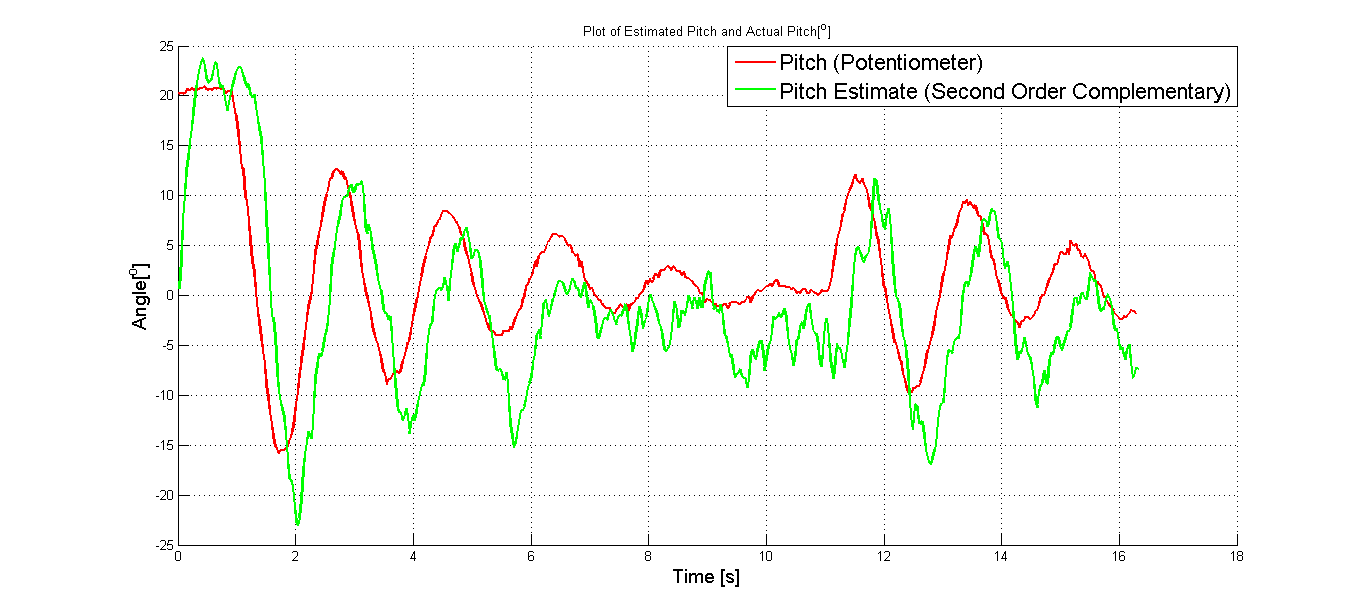
\includegraphics[width =0.38\paperwidth]{\DocRoot/images/comp_sec_time_auto}
		\caption{Time domain response of a Second order Complementary Filter}
		\label{fg: Time domain comparison responce of the sec order comp filter least}
	\end{subfigure}%
	\hspace{3cm}
	\begin{subfigure}{0.32\textwidth}
		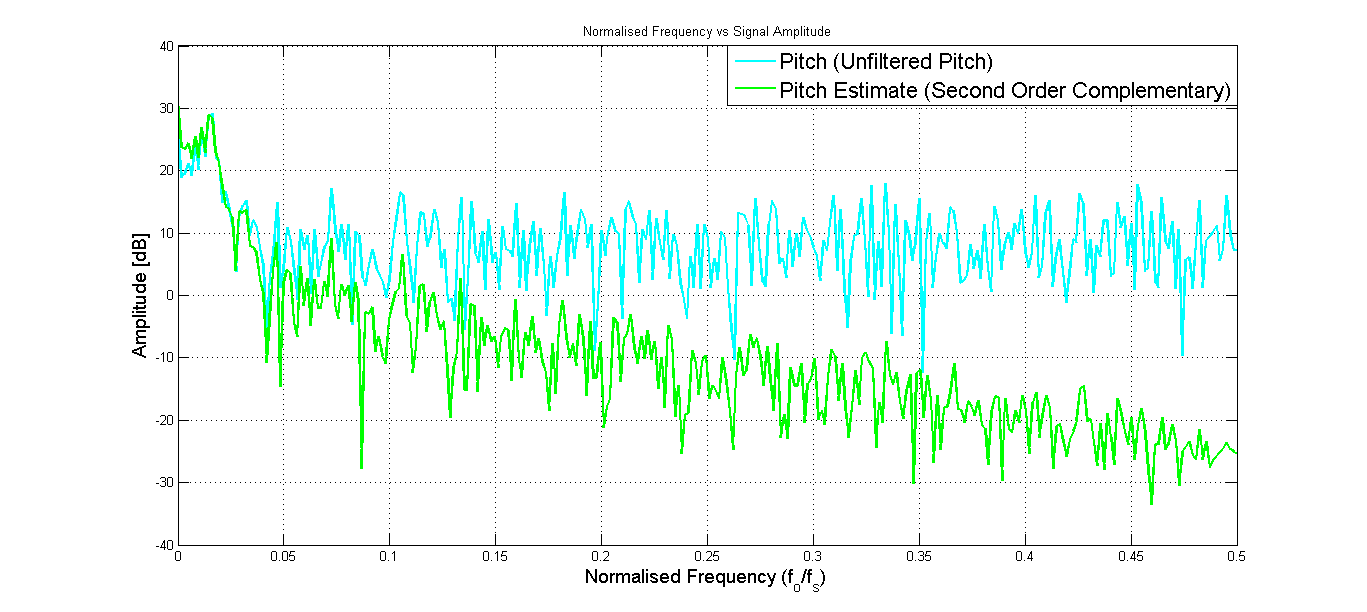
\includegraphics[width =0.38\paperwidth]{\DocRoot/images/comp_sec_fft_least}
		\caption{Frequency domain response of a Second order Complementary Filter}
		\label{fg: Frequency domain responce of the sec order comp filter least}
	\end{subfigure}
	
	\caption{Response of a Second order complementary filter for $K_i = 1.3265$, $K_p = 2.79322$ and ${\gls{ts}} = 30~\mathrm{ms}$ }
	\label{fig sec order comp time and freq responce least}
\end{figure}

\section{Self Tunning Algorithm for a Complementary Filter}

As the \enquote{actual} angle \gls{potangle} of the quad-rotor was known when tuning the filter it was decided to do a search using a \gls{rmse} \eqref{eq:rmse1}. A cross-correlation was done to find the delay between the filtered angle and the \enquote{actual} angle and remove when checking the \gls{rmse} term. This had the best results for the tuned filter and a trade off between lag\footnote{Note with this filter the lag can be set so it does not exceed the maximum allowable phase delay} and filtering could be set. Figure \ref{fig sec order comp time and freq responce auto}	proves that drift on the gyroscope has been removed, but the phase delay of the filtered signal has increased dramatical. 

\begin{equation}
	\gls{rmse} = \sqrt{\frac{\sum_{k = 1}^{n} (\gls{filterdata} -\gls{potangle})^2}{n}} \label{eq:rmse1}
\end{equation}

The cross-correlation function is defined in \eqref{eq: cross-correlation1} and is commonly used in signal processing to find the measure of time-lag between two signals.

\begin{equation}
	(f \star g)[n] = \sum_{m = -\infty}^{\infty} f^*[m]g[m+n] \label{eq: cross-correlation1}
\end{equation}



\begin{algorithm}
	\caption{Auto Tuning a Complementary Filter }\label{Alg: auto tune of comp filter1}
	\begin{algorithmic}[1]
		{	
			\renewcommand{\baselinestretch}{2.5}
			\Procedure{Grid search tuning of a Complementary Filter }{}
			\State Set max value for $K_p$, $K_i$, an \gls{rmse} value and the associated tolerance for the grid.
			
			
			
			\State {\color{white} .}
			\For {length($K_{p(it)}$)} \Comment{$K_{p(it)}$ an array of $K_p$ values to test}
			\State {\color{white} .}
			
			\For {length($K_{i(it)}$}  \Comment{$K_{i(it)}$ an array of $K_i$ values to test}
			\vspace{0.2cm}
			
			\State Calculate \gls{filterdata} the  filtered output using  \eqref{Eq: full dfference equation for the second order filter1}
			\vspace{0.2cm}
			
			\State Calculate Signal Delay of the Filtered output by means of equation \eqref{eq: cross-correlation1} \\ \hspace{2.5cm} by using \gls{filterdata} and \gls{potangle} as it's inputs.
			\vspace{0.2cm}
			\State Remove delay in filtered data by removing samples equal to  the value \\ \hspace{2.5cm}  returned by the previous line of code.
			\vspace{0.2cm}
			\State   Computer the \gls{rmse} value of the filtered signal using equation \eqref{eq:rmse1} \\ \hspace{2.5cm} and \gls{filterdata} \& \gls{potangle} as it's inputs.
			
			\State {\color{white} .}
			\If {(\gls{rmse}  < Previous Error)}
			\State $K_p$ = $K_{p(it)}$(i);
			\State $K_i$ = $K_{i(it)}$ (j);
			\State Previous Error = \gls{rmse};
			\EndIf
			\EndFor
			\EndFor
			
			\State {\color{white} .}
			
			\State \Return {$K_p$ \& $K_i$}
			\EndProcedure}
	\end{algorithmic}
\end{algorithm}

\begin{figure}[h]
	\centering
	\begin{subfigure}{0.32\textwidth}
		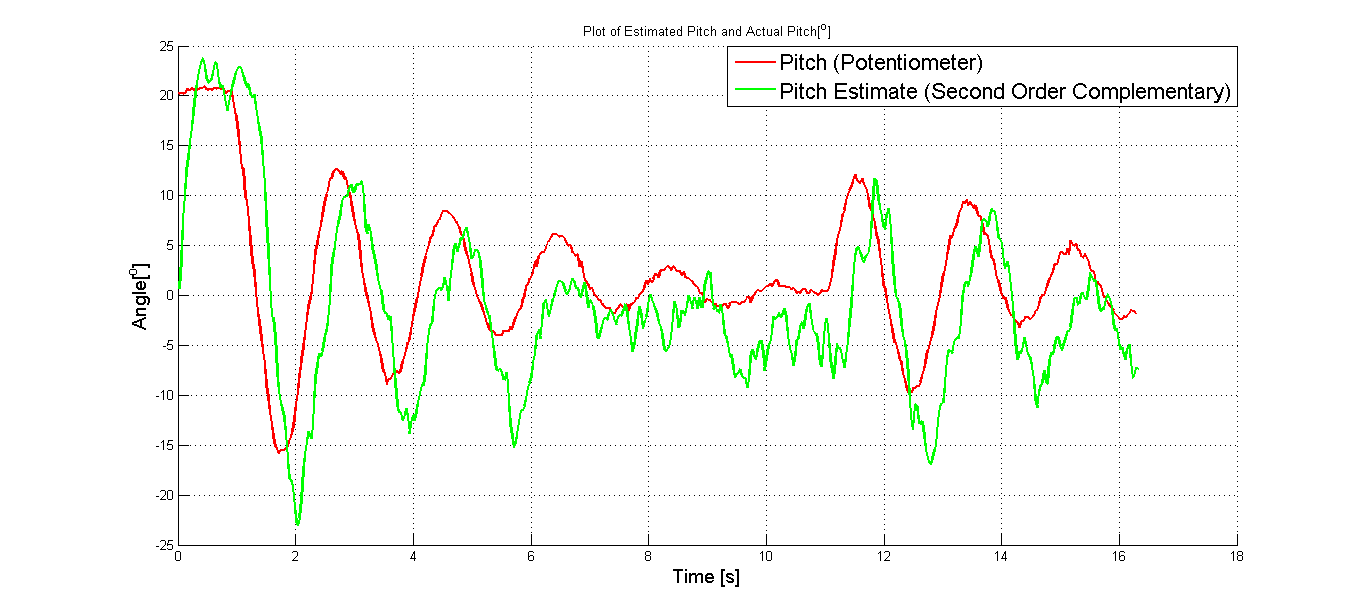
\includegraphics[width =0.38\paperwidth]{\DocRoot/images/comp_sec_time_auto}
		\caption{Time domain response of a Second order Complementary Filter}
		\label{fg: Time domain comparison responce of the sec order comp filter auto}
	\end{subfigure}%
	\hspace{3cm}
	\begin{subfigure}{0.32\textwidth}
		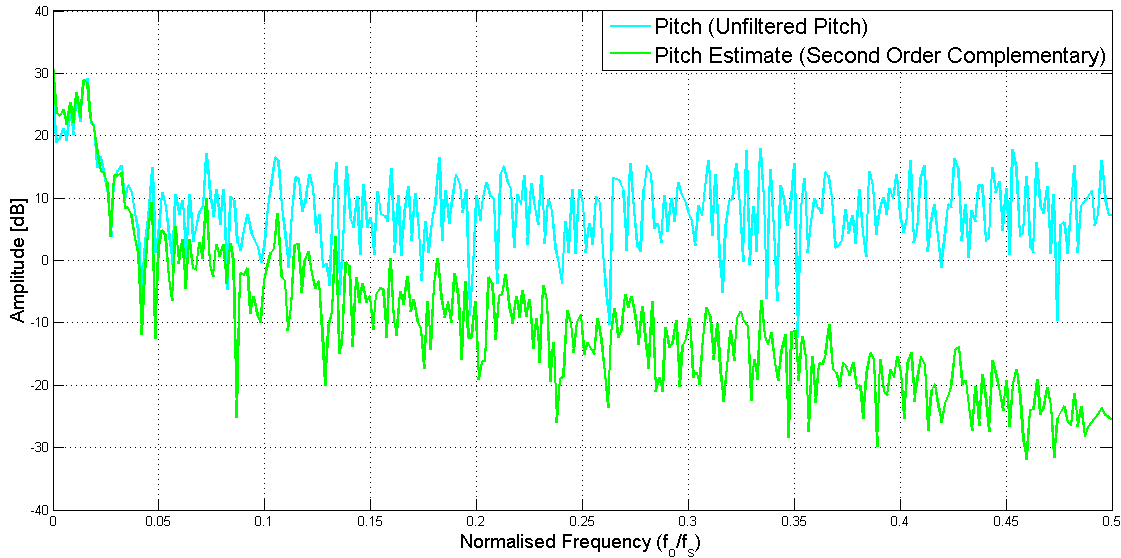
\includegraphics[width =0.38\paperwidth]{\DocRoot/images/comp_sec_fre_auto}
		\caption{Frequency domain response of a Second order Complementary Filter}
		\label{fg: Frequency domain responce of the sec order comp filter auto}
	\end{subfigure}
	
	\caption{Response of a Second order complementary filter for $K_i = 1.2802$, $K_p = 7.1919$ and ${\gls{ts}} = 30~\mathrm{ms}$ }
	\label{fig sec order comp time and freq responce auto}
\end{figure}

As can be seen from Figure \ref{fig sec order comp time and freq responce auto} the second order Complementary Filter removes the bias from the gyroscope, but there is a large delay introduced. Note there is less noise rejection in the second order filter. Hence, another filter was investigated which will be presented next.
\chapter{The Kalman Filter}

In order to design a optimal controller for the quad-rotor a State-Estimator is required. The reason for this is simple: one doesn't have access to all the system states. For example one can't measure the angle velocity of the propellers as the Quad-rotor doesn't have a hall sensor. Due to the use of inexpensive sensors a  stochastic filter or full non-linear model of the sensors had to be developed. Thus, the Kalman Filter was chosen as it is a ideal filter and is capable of estimating angle and rate of change of angle with great accuracy.  \cite{acclerometer_bais}.

\begin{figure}[h]
	\centering
	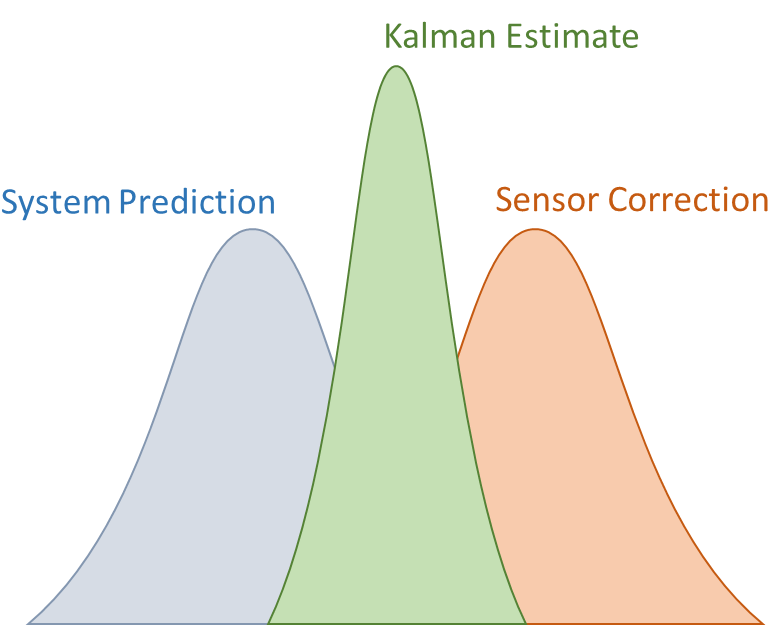
\includegraphics[width =0.4\paperwidth]{\DocRoot/images/kalman_gauss}
	\caption{Gaussian representation of the Kalman Filter}
	\label{Fig: Kalman Filter gauss}
\end{figure}

When a Kalman Filter is being implemented the noise present in the system and senors has to be to Gaussian zero-mean, which is usually denoted as \gls{noiseinsysystem} and \gls{noiseinoutput} respectively. If this criteria is met the filter will yield a new linear system model which is free of noise. The Filter works by adding a prediction produced by the plant model from known inputs, and a correction from the data measured by sensors. This process can be best visualized by figure \ref{Fig: Kalman Filter gauss}, where the plant estimate and the sensor estimate have been fused together to achieve a best guess of the actual state. The Kalman Filter is similar to the Luenberger Observer \footnote{An Observer is used to estimate unmeasurable states by means of a system model and some measurable outputs.}, but the observer gains are chosen in an optimal manner. The Kalman Gain \gls{kalmangain} defines by how much the model estimate has to be corrected by the sensor measurements. Hence, if the noise in the sensors is greater than the noise in the model the senor measurements are trusted more to estimate the required states, and thus assigned a greater weighting. If the noise present in the system states is greater than the noise present in the sensor, then sensor readings will be trusted more to estimate the required states. Thus, in short, the Kalman Filter is a state observer for the stochastic case. In order to apply this filter one must define the system in a discrete liner state space form.

\begin{equation}\label{eq:descrete_state_space_model}
\begin{split}
\underline{x}_{k+1} &= \gls{Transitionmatrix} \underline{x}_k + \gls{Bmatrix}_d\underline{u}_k + \gls{couplingmatrix}\underline{w}_k \\
\underline{z}_{k}      &= \gls{Cmatrix}_d \underline{x}_k + \underline{v}_k
\end{split}
\end{equation}


The filter , whose linear model is described in \ref{eq:descrete_state_space_model}, can be seen as a \gls{lti}  system operating in parallel to the real physical system in order to generate an optimal estimate  $\underline{\hat{x}}$ of all states whereas compensating for the noise in the plant \footnote{Note superscript $d$ notation is dropped for simplicity, E.g ($\gls{Bmatrix} _d~=~ \gls{Bmatrix} $).}. The filter removes/reduces the noise present in the plant by minimizing the error covariance matrix of the estimated states. The covariance matrix is commonly denoted as follows:- 

\begin{equation}
\gls{covariancematrix}= E[\tilde{\underline{x}_k}~{\tilde{\underline{x}_k}}^\top]
\end{equation}
where ${\tilde{\underline{x}}}_k$ is the error in the estimated states.

Note an expression for the \gls{covariancematrix} matrix must be developed from the initial system to begin the filter derivation. Therefore from \eqref{eq:descrete_state_space_model}, the best state estimate can be achieved :-

\[\hat{\underline{x}}_{k+1|k}  =\gls{Transitionmatrix}_k\hat{\underline{x}}_{k|k} + \gls{Bmatrix}{\underline{u}}_k\]


\section{Development of the Kalman Filter}
As seen from figure \ref{fig:Kalman Filter flow diagram} the Kalman Filter is made up of two stages, a predict stage and a correct stage. The predict stage generates an estimate of the required states by means of an ideal system model whose inputs are known. After the estimate is found then the covariance error is measured (this is the aspect to minimize). The covariance error indicates by how much the state estimates differ from the ideal signal. After this the correct stage begins and the Kalman gain \gls{kalmangain} is calculated by means of the covariance error and the covariance of  the sensor data. Next, the initial estimate is corrected by means of sensor data which is scaled appropriately by the Kalman gain \gls{kalmangain}. Finally the covariance error is corrected by means of the Kalman gain \gls{kalmangain} and after which the Kalman starts, hence the recursive aspect of the Kalman Filter.  			


Thus, implement the Kalman filter a recursive algorithm  needs to developed. In order to accomplish this assume access to the previous estimate $\hat{x}_{k|k}$, as the initial value $\hat{x}_{0|0}$ it is possible to define a recursive. If the previous estimate is known any future value can be calculated, but this can only be done if the noise signal is zero mean that is, E[$w_k$] = E[$v_k$] = 0 . Hence, the best estimate can be derived from \eqref{eq:descrete_state_space_model} by taking the mean value of $\underline{w}_k$, doing so will yield the following:-

\begin{equation}
\hat{\underline{x}}_{k+1|k} =\gls{Transitionmatrix}_k\hat{\underline{x}}_{k|k} + \gls{Bmatrix} {\underline{u}}_k
\label{eq: best estimate equation latex}
\end{equation}
Therefore the one-step-ahead  \textit{Predictive measurement} can be defined as follows:-
\begin{equation*}
\hat{z}_{k+1} = \gls{Cmatrix}\hat{x}_{k+1|k}
\end{equation*}

At time (k+1) , one can measure $\gls{measurement}_{+1}$ from the plant, thus define the \textit{Predict error} $\tilde{z}$ as follows:-
\begin{equation}
\tilde{\underline{z}}_{k+1} = {\underline{z}}_{k+1 }- \hat{\underline{z}}_{k+1}
\label{eq: prediction error}
\end{equation}

Thus, to improve the state estimate one can add some proportion of the prediction error \eqref{eq: prediction error} to each element of the state vector to drive the prediction error to zero as follows:-
\begin{equation}
\hat{\underline{x}}_{k+1|k+1}  = \gls{Transitionmatrix}\hat{\underline{x}}_{k|k} +\gls{Bmatrix} {\underline{u}}_k+ \gls{kalmangain}\tilde{\underline{z}}_k
\label{eq: error corrected equation}
\end{equation}

Knowing \eqref {eq: best estimate equation latex},  \eqref{eq: prediction error} and \eqref{eq: error corrected equation} and filling in one gets the following equation:-
\begin{equation}
\hat{\underline{x}}_{k+1|k+1} = \gls{Transitionmatrix}\hat{\underline{x}}_{k|k} +\gls{Bmatrix}{\underline{u}}_{k} + \gls{kalmangain} [{\underline{z}}_{k+1} - { C}(\gls{Transitionmatrix} \hat{\underline{x}}_{k|k} + \gls{Bmatrix}{\underline{u} }_k) ] \label{eq : kalman gain from art of control long}
\end{equation}

Thus matrix/variables are grouped together for ease of computation and yields the following:- 
\begin{equation}
\hat{\underline{x}}_{k+1|k+1} = [{I -\gls{kalmangain}\gls{Cmatrix}}][\gls{Transitionmatrix} \hat{\underline{x}}_{k|k} +\gls{Bmatrix} {\underline{u}}_k] + \gls{kalmangain}z_{k+1} \label{eq: kalman equation from art of controll}
\end{equation}

Equation \ref{eq: kalman equation from art of controll} can be written as follows.
\begin{equation}
\hat{\underline{x}}_{k+1|k+1} = { F}\hat{\underline{x}}_{k|k} + { H}{\underline{u}}_k + \gls{kalmangain}{z}_{k+1} \label{Eq: Kalman Equation Representation used in our reporty}
\end{equation}
Where in \eqref{Eq: Kalman Equation Representation used in our reporty} ${ F} =  [{I -\gls{kalmangain} \gls{Cmatrix} }]\gls{Transitionmatrix}$; $H =  [{I -\gls{kalmangain} \gls{Cmatrix} }] \gls{Bmatrix} $. Thus each matrix is made up of a mix of prediction and correction values.

It was assumed in this project that the separate noise signals were independent of each other, thus allowing \gls{noisecomatrix} and \gls{noisecoplantmatrix} to be covariance matrices. A large value for \gls{noisecomatrix} implies a lot of noise is present in the measurement data and thus more emphasis is placed in the predictions. A large value of \gls{noisecoplantmatrix} implies that there is more noise in the states than in the measurement data and thus the measurement data is followed more closely. As \gls{covariancematrix} is to be minimized, an expression for the estimation of the covariance error can be obtained as follows (\enquote{Predict} stage):-

\begin{equation}
\gls{covariancematrix}^* = \gls{Transitionmatrix}\gls{covariancematrix}_{-1}\gls{Transitionmatrix}^{\intercal} + \gls{couplingmatrix}\gls{noisecoplantmatrix}\gls{couplingmatrix}^{\intercal} \label{eq: P equation for the kalman filter}
\end{equation}

Thus the Kalman gain \gls{kalmangain} can be defined as follows. Note the Kalman Gain \gls{kalmangain} must be updated at each iteration to correct the measurement data so as to obtain an optimal estimate of the required states. The equation governing this update process is as follows (\enquote{Correct} stage) :-

\begin{equation}
\gls{kalmangain}_{k} = \gls{covariancematrix}^*\gls{Cmatrix}^{\intercal}(\gls{Cmatrix}\gls{covariancematrix}^*\gls{Cmatrix}^{\intercal} + \gls{noisecomatrix})^{-1}
\end{equation} 

Finally the covariance error can be corrected as follows:-
\begin{equation}
\gls{covariancematrix} = (I - \gls{kalmangain}_k\gls{Cmatrix})\gls{covariancematrix}^{*}
\end{equation}


From \eqref{eq: P equation for the kalman filter} the performance of this filter depends heavily upon the accuracy of \gls{noisecoplantmatrix} and \gls{noisecomatrix}. Note \gls{noisecomatrix} can often be intelligently estimated from knowledge of the system under control. The derivation of \gls{noisecoplantmatrix} is  a problem as often very little real information will be known about the noise present in the states.  Therefore \gls{noisecoplantmatrix} is often guessed and \gls{noisecomatrix} and \gls{noisecoplantmatrix} are tuned together to get an adequate result for the control of the device.
\begin{comment}
	\tikzset{%
	block/.style    = {draw, thick, rectangle, minimum height = 3em,minimum width = 3em},
	
	input/.style    = {coordinate}, % Input
	
	output/.style   = {coordinate} % Output

	block/.style    = {draw, thick, rectangle, minimum height = 3em,minimum width = 3em},

	gain/.style     = {draw, thick, isosceles triangle, minimum height = 2em,isosceles triangle apex angle=60},

	port/.style     = {inner sep=0pt, font=\tiny},
	
	sum/.style n args = {4}{draw, circle, node distance = 2cm, minimum size=5mm, alias=sum,
		append after command={
			node at (sum.north) [port, below=1pt] {$#1$}
			node at (sum.west) [port, right=1pt] {$#2$}
			node at (sum.south) [port, above=1pt] {$#3$}
			node at (sum.east) [port, left=1pt] {$#4$}
		},
	}, % Adder
	
	joint/.style    = {circle, draw, fill, inner sep=0pt, minimum size=2pt},
	
}
% Defining string as labels of certain blocks.
\newcommand{\suma}{\Large$+$}
\newcommand{\inte}{$\displaystyle \int$}
\newcommand{\derv}{\huge$\frac{d}{dt}$}
\end{comment}

\subsection{Kalman Filter Operation}

As described in the previous sections, the Kalman Filter extracts state estimates from noisy signals. This can be done by obtaining statistical information of the noise present in both the plant and the measurement data, knowing this the filter can optimally estimate the state of interest. This information is given in form of the plant and measurement noise covariances, \gls{noisecomatrix} and \gls{noisecoplantmatrix}. The algorithm that the filter performs can be described as follows:


First, the \gls{noisecoplantmatrix} and \gls{noisecomatrix} covariance matrices are calculated through trial and error. An initial state estimate $\hat{\underline{x}}_{0|0}$ and its error covariance $\text{\bf P}_0$ are entered. The Kalman Gain matrix, \gls{kalmangain} is computed based on \text{\bf P}, \gls{noisecomatrix} and the transition matrix \gls{Transitionmatrix}. The estimate is then updated with the current measurement data and after which a new error covariance computed. The algorithm then starts again from the beginning. The output from the filter is an estimate of the states and the error covariance matrix, {\bf P}. Figure \ref{fig:Kalman Filter flow diagram}, shown below is a flow diagram of the Kalman Filter algorithm.   


		\begin{figure}[h]
			\renewcommand{\baselinestretch}{1.5} 	
			\centering
			\resizebox{14cm}{8cm}{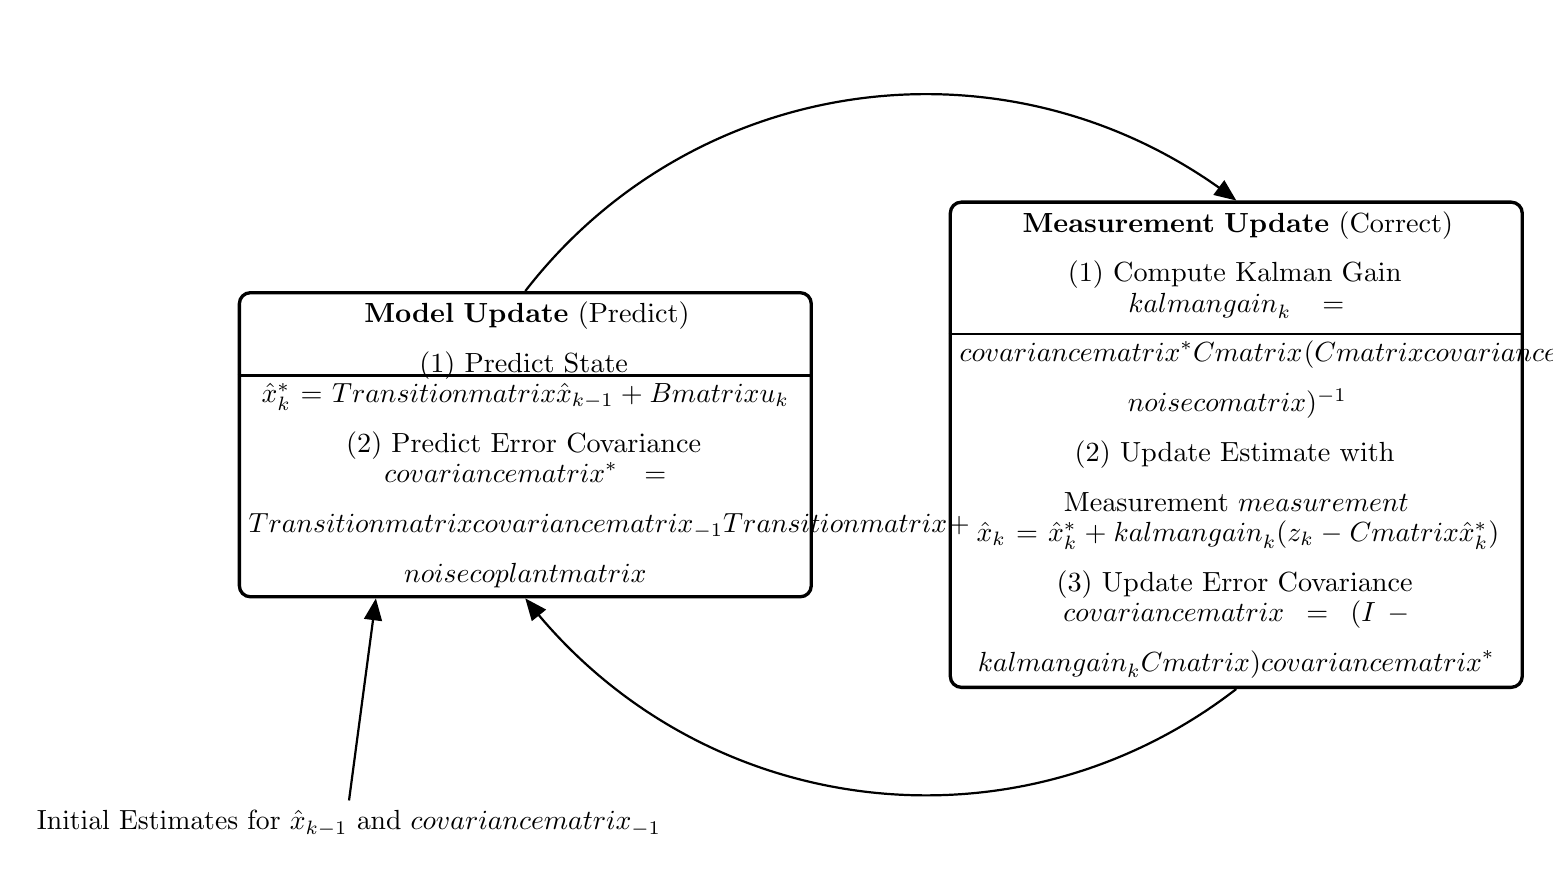
\begin{tikzpicture}[auto, thick, node distance=2cm, >=triangle 45]
			
			%
			% Styles for states, and state edges
			%
			\tikzstyle{state} = [{rectangle, rounded corners, draw=black, very thick, text width=20.0em, minimum height=4em, text centered}]
			\tikzstyle{stateEdgePortion} = [black,thick];
			\tikzstyle{stateEdge} = [stateEdgePortion,->];
			\tikzstyle{edgeLabel} = [pos=0.5, text centered, font={\sffamily\small}];
			
			
			%
			% Position States
			%
			\node[state, name=predict] {{{\LARGE}{\bf Model Update} (\enquote{Predict})}   \\ 
				{   (1) Predict State  \\  \vspace{-0.25cm}
					\hh $\hat{x}^{*}_{k} = \gls{Transitionmatrix}\hat{x}_{k-1} + \gls{Bmatrix}u_{k}$\\ 
					(2) Predict Error Covariance \\ \vspace{-0.25cm}
					\hh $\gls{covariancematrix}^* = \gls{Transitionmatrix}\gls{covariancematrix}_{-1}\gls{Transitionmatrix}^{\intercal} + \gls{noisecoplantmatrix}$}};
			
			
			\node[state, name=correct, right of=predict, xshift=20em] {{\bf Measurement Update} (\enquote{Correct}) \\ 
				{   (1) Compute Kalman Gain\\  \vspace{-0.25cm}
					\hh $\gls{kalmangain}_{k} = \gls{covariancematrix}^*\gls{Cmatrix}^{\intercal}(\gls{Cmatrix}\gls{covariancematrix}^*\gls{Cmatrix}^{\intercal} + \gls{noisecomatrix})^{-1}$\\ 
					(2) Update Estimate with Measurement $\gls{measurement}$ \\ \vspace{-0.25cm}
					\hh $\hat{x}_k = \hat{x}^{*}_k + \gls{kalmangain}_k(z_k - \gls{Cmatrix}\hat{x}_k^{*})$\\
					(3) Update Error Covariance  \\ \vspace{-0.25cm}
					\hh $\gls{covariancematrix} = (I - \gls{kalmangain}_k\gls{Cmatrix})\gls{covariancematrix}^{*}$
					
				}};
				
				
				%
				% Connect States via edges
				%
				\draw (predict.north) 
				edge[stateEdge, bend left=45] node[edgeLabel, xshift=-3em]{} 
				(correct.north); 
				
				\draw ($(predict.west) + (0,2.5em)$) 
				edge[stateEdgePortion] node[edgeLabel, yshift=+2.1cm]{} 
				($(predict.east) + (0,2.5em)$); 
				
				\draw (correct.south) 
				edge[stateEdge, bend left=45] node[edgeLabel, xshift=-3em]{} 
				(predict.south); 
				
				\draw ($(correct.west) + (0,4.0em)$) 
				edge[stateEdgePortion] node[edgeLabel, yshift=+2.1cm]{} 
				($(correct.east) + (0,4.0em)$); 
				
				
				
				% 
				% inital states to start the filter
				%
				\node[ name=inital, below of=predict, left of=predict, xshift = -0.68em ,yshift=-8em]{Initial Estimates for $\hat{x}_{k-1}$ and $\gls{covariancematrix}_{-1}$};
				
				\draw ($(inital.north) + (0,0)$) 
				edge[stateEdge] node[edgeLabel, yshift=+2.1cm]{} 
				($(predict.south) + (-5.4em,0)$); 
				\end{tikzpicture}}
					\caption{Kalman Filter flow diagram}
					\label{fig:Kalman Filter flow diagram}
			\end{figure}




\section{Kalman Filter Used in Project}
 There were three Kalman filters developed for this report; a steady state Kalman Filter whose Kalman Gains remains constant over time, a Kinematic Kalman Filter which is based on the Kalman filter presented in Ersson and Hu \cite{ersson2001state} and an Extended Kalman Filter. Note all Kalman Filters investigated in this project will be developed in this section, while the implementation and tuning will be presented in Chapter \ref{chap: kalman implem}

\subsection{The Static Kalman Filter}
The Static Kalman Filter, which will be developed in the this sections uses a constant \gls{kalmangain} which is found by means of the Kalman Filter Algorithm presented in \ref{fig:Kalman Filter flow diagram}. In practice, the time-varying Kalman gain \gls{kalmangain} tends towards a steady value \cite{LQG_mit}. Hence, when the Kalman Filter is used on the quad-rotor the Kalman Gain \gls{kalmangain} will converge to a constant value, thus, a constant Kalman Gain \gls{kalmangain} can be used to estimate the required states. As the Static Kalman Filter uses a constant \gls{kalmangain} term, the observer produced by this method is a optimal Luenberger Observer\footnote{This Static Kalman Gain can be found by using the \textit{lqg} commend in MatLab}. The model used in the Kalman Filter for the pitch, roll and yaw axes are the same ones developed in \eqref{eq: pitch model}, \eqref{eq: roll model} and \eqref{d2ydt2}. Note as these are continuous equations, a mapping of the continuous time model to a discrete model has to take place which was done by means of the Matrix Exponential. After the discrete Static Kalman Filter was developed the \gls{kalmangain} terms shown in \eqref{eq: static kalman equations for micro} was adjusted by methods presented in Chapter \ref{chap: kalman implem} until an optimal response was achieved. 
\subsection{Derivation of state space equations}
As the Kalman Filter is required run on a micro-controller, the Kalman Filter expressed in  \ref{Eq: Kalman Equation Representation used in our reporty} has to be expressed in its most compact format so as to reduce computational effort and improve its accessibility. These requirement lead to the following definition for the Static Kalman Filter:-
%{Eq: Kalman Equation Representation used in our reporty}
\begin{equation}
\begin{bmatrix}																
\hat{x}_1		         			\\
\hat{ x}_2		
\end{bmatrix}_{k+1}
=
\begin{bmatrix}
F_{11}	& F_{12 } \\
F_{21}	& F_{22}
\end{bmatrix}
\begin{bmatrix}											
\hat{ x}_1		         			\\
\hat{ x}_2		
\end{bmatrix}_{k}	
+
\begin{bmatrix}
H_1 \\
H_2
\end{bmatrix}
{ u}_k
+
\begin{bmatrix}
K_{11}	& K_{12 } \\
K_{21}	& K_{22}
\end{bmatrix}
\begin{bmatrix}											
{ z}_1		         			\\
{z}_2		
\end{bmatrix}_{k+1}	
\label{eq: static kalman equations for micro}
\end{equation}

For the quad-rotor the state ${ x_1}$ is angular velocity ${\bf \alpha}$ and the state ${ x_2}$ is angular acceleration $\dot{\bf \alpha}$  


\subsection{The Kinematic Kalman Filter}
Unlike the Kalman Filter presented in the previous section, the Kalman filter being developed in the following section uses a pure kinematic relationship, thus a model of the plant is not required. This kinematic relationship uses the current gyroscope data to relate the derivative of the rotation matrix to the rotation matrix and is defined as follows:-

\begin{equation}
\dot{\gls{rotationmatrix}} =  \underbrace{\left[\begin{array}{ccc} 0 & \gls{wz} & -\gls{wy}\\ -\gls{wz} & 0 & \gls{wx}\\ \gls{wy}&-\gls{wx} & 0 \end{array}\right] }_{\text{\gls{skewmatrix}}}\gls{rotationmatrix}  \label{eq: rotation matrix related using the gyro readings}
\end{equation} 




\begin{description}[itemsep=0.5mm]
	\item[{\bf Where:-}]
	\item[\gls{skewmatrix}:] is a skewed matrix that contains the set of all proper orthogonal matrices and is defined as {$\gls{skewmatrix} \bf= R|R\varepsilon R^{3x3},R^\intercal R = RR^\intercal = I$}
	\item[\gls{wx}, \gls{wy}, \gls{wz}:] are the roll,pitch and yaw angular rates, respectively.
\end{description}

These rates are measured using the gyroscopes onboard the quad-rotor, in the \gls{imu}.

Using \eqref{eq: rotation matrix related using the gyro readings}, the following continuous state space equations presented in \eqref{eq:state space adative kalman equations1} can be used to  represent the system:-
 


\begin{align}
\begin{split}
\dot{\underline{x}} &= \gls{skewmatrix}\underline{x}\\
\underline{y}              &= \underline{x}
\end{split}
\label{eq:state space adative kalman equations1}
\end{align}

However, \eqref{eq:state space adative kalman equations1} is a continuous state space equation. This must be converted to the discrete version since the Kalman Filter must be implemented in discrete form, which is achieved as follows:-

\begin{align}
\begin{split}
\underline{x}_k &= \gls{Transitionmatrix}_k x_{k-1}\\
\underline{y}_k              &= \underline{x}_k
\end{split}
\end{align}



The transformation from the continuous to discrete form is shown in appendix \ref{chap: Rotation Matrix reation}. $\gls{Transitionmatrix}_k$ = $e^{\gls{skewmatrix}\gls{ts}}$, where \gls{ts} is the sampling time of the system. Since \gls{rotationmatrix} is a rotation matrix, and $\underline{x}$ is a column of \gls{Transitionmatrix} (for reasons defined in Section \ref{sec: acc model}). In this filter the dynamic component of the accelerometer measurement is considered to be a disturbance and is assumed to be Gaussian. It is therefore treated as noise and must be removed so as to acquire an accurate estimate. After the noise has been removed from the accelerometer output \eqref{Eq: angles from acc1} can be used to estimate the attitude of the quad-rotor.



\begin{figure}[h]
	\centering
	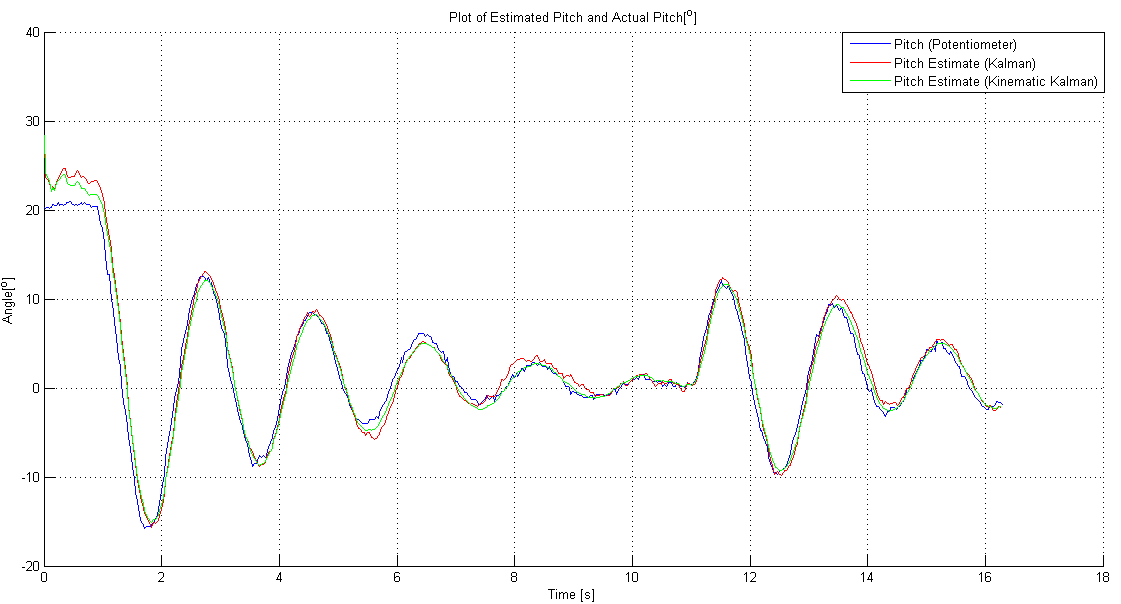
\includegraphics[width =0.7\paperwidth]{\DocRoot/images/kalman_filter_comparsion}
	\caption{Plot of Kalman Filter Estimate, Kinematic Kalman Filter Estimate and Actual Angle of the device}
	\label{Fig: Kalman Filter Estimate and Kinematic Kalman Filter Estimate1}
\end{figure}




\subsection{The Extended Kalman Filter }
As the gyroscope measurement function $h(x_k,\gls{noiseinoutput}_k)$ is highly non-linear it was decided that it was worth while looking at a more advanced Kalman Filter which is capable of dealing with non-linear systems: thus the Extended Kalman Filter was explored (see section \ref{sec: gyroscope sec} for more details on the gyroscope measurement function). Also, as a \gls{gps} module is required to implement positional controller on the quad-rotor it was the natural choice to investigate the \gls{ekf} as it is the de-facto filter used in such systems \cite{An_Introduction_to_the_Kalman_Filter}. 






As the \gls{ekf} filters non-linear functions by means of linearizion of the system around the current
estimate, a method of finding the partial derivatives of both the process and measurement functions is required. Hence, if the process is governed by the \textit{non-linear} stochastic difference equation:-
\begin{equation}
x_k = f(x_{k-1},u_k,\gls{noiseinsysystem}_{k-1})
\end{equation}
and the measurement model by the following stochastic difference equation:-
\begin{equation}
z_k = h(x_k,\gls{noiseinoutput}_k)
\end{equation}

where the random variables \gls{noiseinsysystem} and \gls{noiseinoutput} again represent the process and measurement
noise.



In practice individual values of the individual \gls{noiseinsysystem} and \gls{noiseinoutput}change at each time step. However, one can approximate the state and measurement  without
them as follows:-

\begin{equation}
x_k^* = f(\hat{x}_{k-1},u_k,0) \label{eq: ekf approximate the state}
\end{equation}
Next the measurement model  can be defined by means of the following stochastic difference equation:-
\begin{equation}
z_k = h(x_k^*,0)  \label{eq: ekf approximate the measurement}
\end{equation}

It is important to note that a fundamental flaw of the \gls{ekf} is that the distributions of the various random variables are no longer normal
after undergoing their respective non-linear transformations. The \gls{ekf} is simply an ad-hoc estimator. The \gls{ekf} only approximates the optimality of Bayes’ rule by linearization.


Equation \eqref{eq: ekf approximate the state} is linearized around the control input $u_k$ and the previous estimate using \eqref{eq: jacobain of fx} and the measurement function \eqref{eq: ekf approximate the measurement} is linearized around the $x_k^*$  using  \eqref{eq: jacobain of hx}
\begin{equation}
A_k=\left.\left[\begin{array}{cccc}
\frac{\partial f_{1}}{\partial x_1} &\frac{\partial f_{1}}{\partial x_2} &\dots& \frac{\partial f_{1}}{\partial x_n}\\
\frac{\partial f_{2}}{\partial x_1} &\frac{\partial f_{2}}{\partial x_2} &\dots& \frac{\partial f_{2}}{\partial x_n}\\
\vdots& \vdots& \ddots &\vdots\\
\frac{\partial f_{n}}{\partial x_1} &\frac{\partial f_{n}}{\partial x_2} &\dots&\frac{\partial f_{n}}{\partial x_n} \\
\end{array}\right]\right|_{\hat{x}_k,u_k} \label{eq: jacobain of fx}
\end{equation}

\begin{equation}
C_k=\left.\left[\begin{array}{cccc}
\frac{\partial h_{1}}{\partial x_1} &\frac{\partial h_{1}}{\partial x_2} &\dots& \frac{\partial h_{1}}{\partial x_n}\\
\frac{\partial h_{2}}{\partial x_1} &\frac{\partial h_{2}}{\partial x_2} &\dots& \frac{\partial h_{2}}{\partial x_n}\\
\vdots& \vdots& \ddots &\vdots\\
\frac{\partial h_{n}}{\partial x_1} &\frac{\partial h_{n}}{\partial x_2} &\dots&\frac{\partial h_{n}}{\partial x_n} \\
\end{array}\right]\right|_{\hat{x}_k^*} \label{eq: jacobain of hx}
\end{equation}

Note the above Jacobian can be approximated at each stage on a micro-controller by using the Cauchy’s integral
formula which is defined as follows\cite{Jacobain_approx_paper}:-


\begin{equation}
f^{(n)}(z) = \frac{n!}{2\pi i}\oint_\gamma \frac{f(\kappa)}{(\kappa - z)^{n+1}}d\kappa \label{eq: Cauchy's intrgral formula}
\end{equation}
To implement \eqref{eq: Cauchy's intrgral formula} on a micro-controller it must be approximated as follows:-

\begin{equation}
f^{(n)}(z) \approx \frac{n!}{mh} \sum_{j=0}^{m-1}\frac{f(z+h e^{i\frac{2 \pi j}{m}})}{e^{i\frac{2 \pi j n}{m}}}
\end{equation}

The derivation of a complex-step derivative (first partial derivative) approximation is done by an approximation of a non-linear function with a complex variable using the Taylor's series expansion.

\begin{equation}
f(x+ih) = f(x) + ihf^{'} (x) - h^2\frac{f^{''}(x)}{2!}- ih^3\frac{f^{'''}(x)}{3!}+h^4\frac{f^{4}(x)}{4!} + \dots
\end{equation}
Now taking only the imaginary parts of both sides gives

\begin{equation}
\mathrm{Im}[f(x+ih)] = hf^{'}(x) - h^3\frac{f^{'''}(x)}{3!}+\dots \label{eq: imaginary parts of  Cauchys integral approx}
\end{equation}
Dividing by $h$, rearranging and assuming terms higher than $h^2$ can be ignored since the interval $h$ can be chosen up to the precision of the machine (smallest number the machine can produce) and thus \eqref{eq: imaginary parts of  Cauchys integral approx} can be approximated as follows:-
\begin{equation}
f^{'}(x) = \mathrm{Im}[f(x+ih)]/h \label{eq: how to do differenation on a controller}
\end{equation}
As \eqref{eq: how to do differenation on a controller} is not a function of differences it is more accurate than standard finite difference and more importantly partial derivative can be calculated on a micro-controller using \eqref{eq: how to do differenation on a controller}. 

As a method of approximating the Jacobian matrix has been presented in \eqref{eq: how to do differenation on a controller}, it is now possible to implement the \gls{ekf} on a micro-controller. As the computational capabilities of the micro-controller used in this project were insufficient of implementing an \gls{ekf} it was decided to only simulate the filter. The \gls{ekf} was implemented in MatLab using the algorithm presented in figure \ref{fig: Extended Kalman Filter flow diagram}, and the filtered results can be seen in Figure \ref{Fig:Cross-Correlation of estimated pitch error1}. As can be seen from Figure \ref{Fig:Cross-Correlation of estimated pitch error1} produces the best estimate of the attitude of the quad-rotor; this means an \gls{ekf} would be the ideal filter for both attitude estimation of the quad-rotor as well as \gls{gps} position estimation of the quad-rotor. 


\begin{figure}[h]
	\renewcommand{\baselinestretch}{1.5} 	
	\centering
	\resizebox{16cm}{10cm}{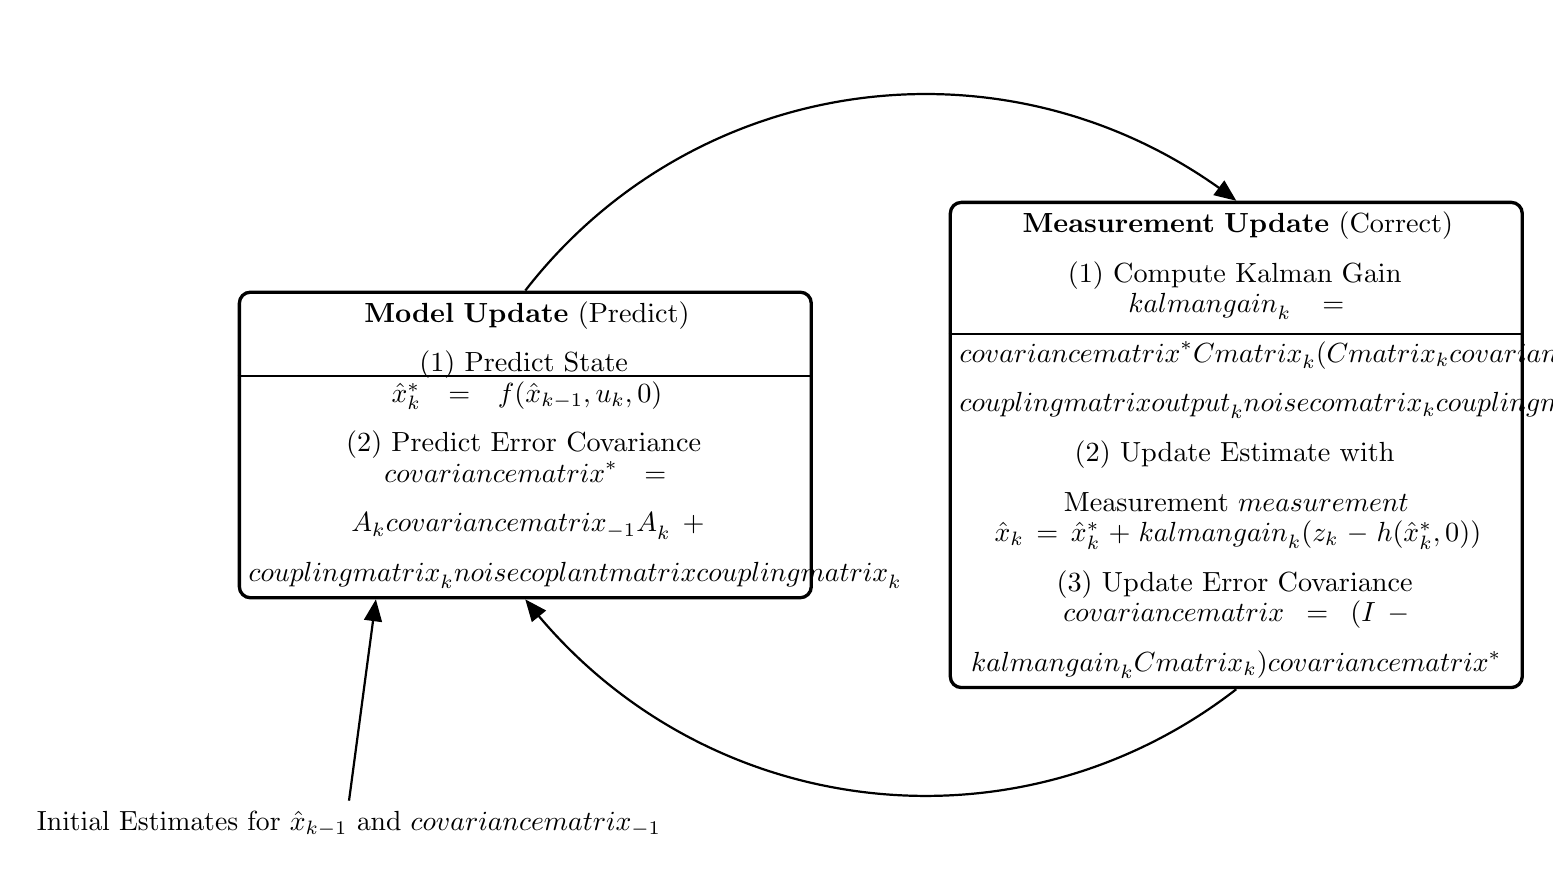
\begin{tikzpicture}[auto, thick, node distance=2cm, >=triangle 45]
	%
	% Styles for states, and state edges
	%
	\tikzstyle{state} = [{rectangle, rounded corners, draw=black, very thick, text width=20.0em, minimum height=4em, text centered}]
	\tikzstyle{stateEdgePortion} = [black,thick];
	\tikzstyle{stateEdge} = [stateEdgePortion,->];
	\tikzstyle{edgeLabel} = [pos=0.5, text centered, font={\sffamily\small}];
	
	
	%
	% Position States
	%
	\node[state, name=predict] {{{\LARGE}{\bf Model Update} (\enquote{Predict})}   \\ 
		{   (1) Predict State  \\  \vspace{-0.25cm}
			\hh $\hat{x}^{*}_{k} = f(\hat{x}_{k-1},u_k,0)$\\ 
			(2) Predict Error Covariance \\ \vspace{-0.25cm}
			\hh $\gls{covariancematrix}^* = A_k\gls{covariancematrix}_{-1}A_k^{\intercal} + \gls{couplingmatrix}_k\gls{noisecoplantmatrix}\gls{couplingmatrix}_k^{\intercal}$}};
	
	
	\node[state, name=correct, right of=predict, xshift=20em] {{\bf Measurement Update} (\enquote{Correct}) \\ 
		{   (1) Compute Kalman Gain\\  \vspace{-0.25cm}
			\hh $\gls{kalmangain}_{k} = \gls{covariancematrix}^*\gls{Cmatrix}_k^{\intercal}(\gls{Cmatrix}_k\gls{covariancematrix}^*\gls{Cmatrix}_k^{\intercal} + \gls{couplingmatrixoutput}_k\gls{noisecomatrix}_k\gls{couplingmatrixoutput}_k^{\intercal})^{-1}$\\ 
			(2) Update Estimate with Measurement $\gls{measurement}$ \\ \vspace{-0.25cm}
			\hh $\hat{x}_k = \hat{x}^{*}_k + \gls{kalmangain}_k(z_k - h(\hat{x}^{*}_{k},0))$\\
			(3) Update Error Covariance  \\ \vspace{-0.25cm}
			\hh $\gls{covariancematrix} = (I - \gls{kalmangain}_k\gls{Cmatrix}_k)\gls{covariancematrix}^{*}$
			
		}};
		
		
		%
		% Connect States via edges
		%
		\draw (predict.north) 
		edge[stateEdge, bend left=45] node[edgeLabel, xshift=-3em]{} 
		(correct.north); 
		
		\draw ($(predict.west) + (0,2.5em)$) 
		edge[stateEdgePortion] node[edgeLabel, yshift=+2.1cm]{} 
		($(predict.east) + (0,2.5em)$); 
		
		\draw (correct.south) 
		edge[stateEdge, bend left=45] node[edgeLabel, xshift=-3em]{} 
		(predict.south); 
		
		\draw ($(correct.west) + (0,4.0em)$) 
		edge[stateEdgePortion] node[edgeLabel, yshift=+2.1cm]{} 
		($(correct.east) + (0,4.0em)$); 
		
		

		
		
		% 
		% inital states to start the filter
		%
		\node[ name=inital, below of=predict, left of=predict, xshift = -0.68em ,yshift=-8em]{Initial Estimates for $\hat{x}_{k-1}$ and $\gls{covariancematrix}_{-1}$};
		
		\draw ($(inital.north) + (0,0)$) 
		edge[stateEdge] node[edgeLabel, yshift=+2.1cm]{} 
			($(predict.south) + (-5.4em,0)$); 
		\end{tikzpicture}}
\caption{Extended Kalman Filter flow diagram}
\label{fig: Extended Kalman Filter flow diagram}
\end{figure}

\begin{figure}[h]
	\centering
	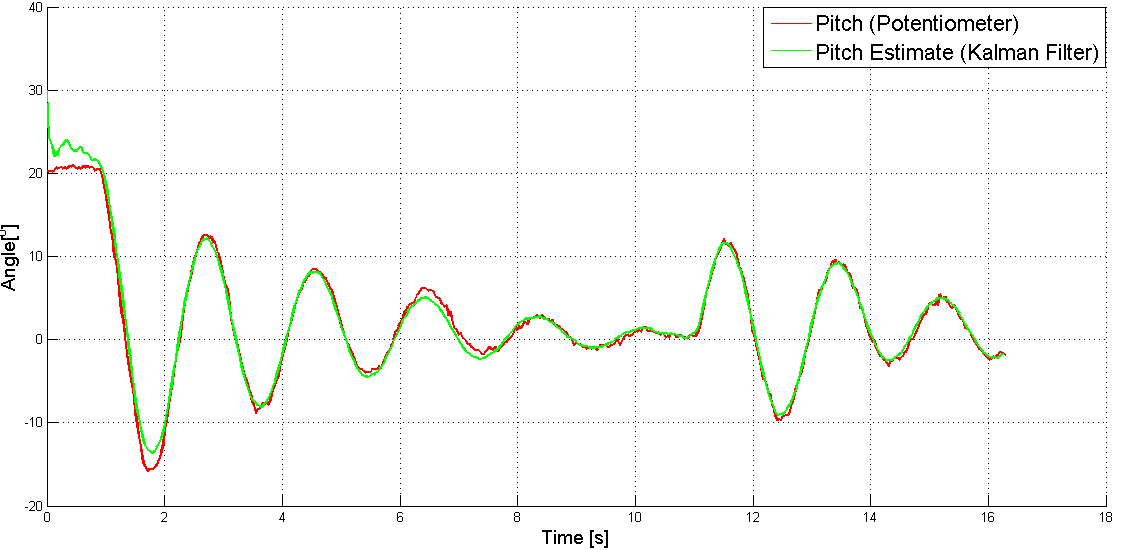
\includegraphics[width =0.8 \paperwidth]{\DocRoot/images/Kalman_low}
	\caption{Time-domain response of the Extended Kalman Filter}
	\label{Fig:Cross-Correlation of estimated pitch error1}
\end{figure}





\begin{comment}
\begin{figure}[h]
\renewcommand{\baselinestretch}{1.5} 	
\centering
\resizebox{14cm}{8cm}{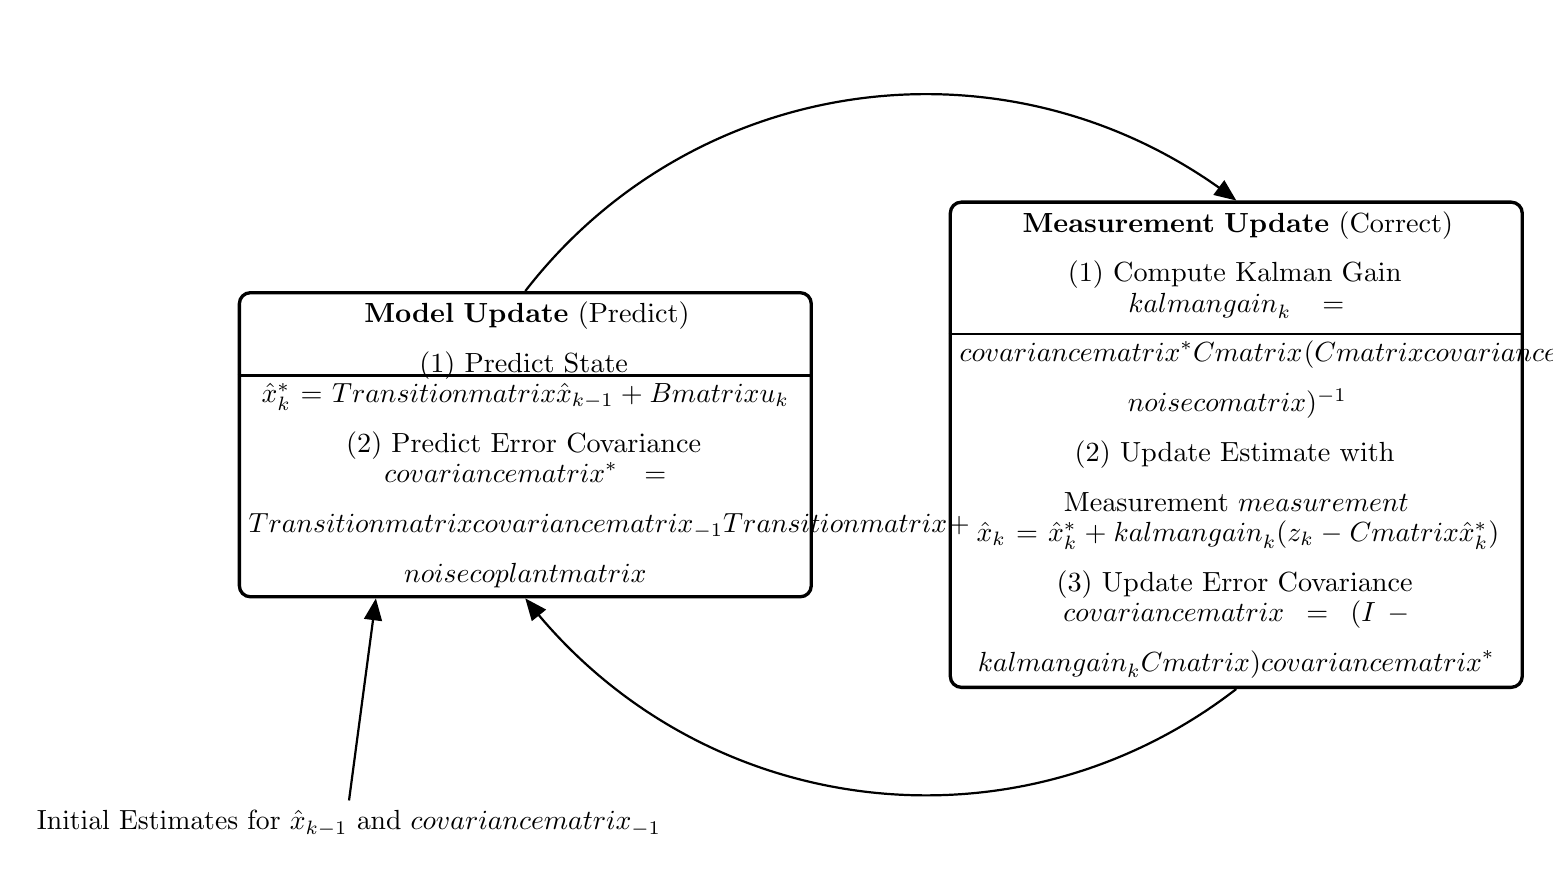
\begin{tikzpicture}[auto, thick, node distance=2cm, >=triangle 45]

%
% Styles for states, and state edges
%
\tikzstyle{state} = [{rectangle, rounded corners, draw=black, very thick, text width=20.0em, minimum height=4em, text centered}]
\tikzstyle{stateEdgePortion} = [black,thick];
\tikzstyle{stateEdge} = [stateEdgePortion,->];
\tikzstyle{edgeLabel} = [pos=0.5, text centered, font={\sffamily\small}];


%
% Position States
%
\node[state, name=predict] {{{\LARGE}{\bf Model Update} (\enquote{Predict})}   \\ 
{   (1) Predict State  \\  \vspace{-0.25cm}
\hh $\hat{x}^{*}_{k} = \gls{Transitionmatrix}\hat{x}_{k-1} + \gls{Bmatrix}u_{k}$\\ 
(2) Predict Error Covariance \\ \vspace{-0.25cm}
\hh $\gls{covariancematrix}^* = \gls{Transitionmatrix}\gls{covariancematrix}_{-1}\gls{Transitionmatrix}^{\intercal} + \gls{noisecoplantmatrix}$}};


\node[state, name=correct, right of=predict, xshift=20em] {{\bf Measurement Update} (\enquote{Correct}) \\ 
{   (1) Compute Kalman Gain\\  \vspace{-0.25cm}
\hh $\gls{kalmangain}_{k} = \gls{covariancematrix}^*\gls{Cmatrix}^{\intercal}(\gls{Cmatrix}\gls{covariancematrix}^*\gls{Cmatrix}^{\intercal} + \gls{noisecomatrix})^{-1}$\\ 
(2) Update Estimate with Measurement $\gls{measurement}$ \\ \vspace{-0.25cm}
\hh $\hat{x}_k = \hat{x}^{*}_k + \gls{kalmangain}_k(z_k - \gls{Cmatrix}\hat{x}_k^{*})$\\
(3) Update Error Covariance  \\ \vspace{-0.25cm}
\hh $\gls{covariancematrix} = (I - \gls{kalmangain}_k\gls{Cmatrix})\gls{covariancematrix}^{*}$

}};


%
% Connect States via edges
%
\draw (predict.north) 
edge[stateEdge, bend left=45] node[edgeLabel, xshift=-3em]{} 
(correct.north); 

\draw ($(predict.west) + (0,2.5em)$) 
edge[stateEdgePortion] node[edgeLabel, yshift=+2.1cm]{} 
($(predict.east) + (0,2.5em)$); 

\draw (correct.south) 
edge[stateEdge, bend left=45] node[edgeLabel, xshift=-3em]{} 
(predict.south); 

\draw ($(correct.west) + (0,4.0em)$) 
edge[stateEdgePortion] node[edgeLabel, yshift=+2.1cm]{} 
($(correct.east) + (0,4.0em)$); 



% 
% inital states to start the filter
%
\node[ name=inital, below of=predict, left of=predict, xshift = -0.68em ,yshift=-8em]{Initial Estimates for $\hat{x}_{k-1}$ and $\gls{covariancematrix}_{-1}$};

\draw ($(inital.north) + (0,0)$) 
edge[stateEdge] node[edgeLabel, yshift=+2.1cm]{} 
($(predict.south) + (-5.4em,0)$); 
\end{tikzpicture}}
\caption{Kalman Filter flow diagram}
\label{fig:Kalman Filter flow diagram}
\end{figure}























\subsection{Block Diagram of the Kalman filter}
\pgfmathsetmacro{\lowergroup}{-8}
\pgfmathsetmacro{\lowerlowergroup}{-9.5}
\pgfmathsetmacro{\lqr}{-5.5}
\pgfmathsetmacro{\joint}{-6.5}
\pgfmathsetmacro{\cd}{-4.0}
\pgfmathsetmacro{\k}{-5.0}
\pgfmathsetmacro{\endpoint}{10}
\pgfmathsetmacro{\endpointtwo}{12}
\pgfmathsetmacro{\endpointthree}{14}
\pgfmathsetmacro{\noise}{1.5}
\begin{figure}[h]	
	\centering
	\begin{tikzpicture}[auto, thick, node distance=2cm, >=triangle 45]
	\draw
	% Drawing the blocks of first filter :
	node at (-0.3,0)     {$R$} 
	node at (5,2.3)     {\text{\footnotesize   Zero Mean Process Noise}} 
	node at (\endpointtwo+2,2.3)     {\text{\footnotesize  Zero Mean Measurement Noise}} 
	node at (3.2,\noise)      {\gls{noiseinsysystem}}
	node at (\endpointthree,\noise)      {\gls{noiseinoutput}}
	
	node at (0,0)      [input,name=input1,thick,above]{} 
	node at (3.5,\noise)      [input,name=noisesys,thick,above]{}
	node at (\endpointthree-.3,\noise)     [input,name=noisemea,thick,above]{}
	
	node at (1,0)              [sum={}{+}{-}{}]  (sum1) {}
	node at (6,0)              [sum={+}{+}{+}{}] (sum2) {}
	node at (\endpointtwo,0)             [sum={+}{+}{}{}]  (sum3) {}
	node at (\endpoint,\lowergroup)   [sum={}{+}{}{+}]  (sum4) {}
	node at (\endpointthree,\cd)           [sum={+}{-}{}{}]  (sum5) {}
	node at (\endpointthree,\joint)        [sum={+}{+}{}{}]  (sum6) {}
	
	node at (8,0) [block,scale=0.8](delay) {$q^{-1}$}
	node at (6,\lowergroup) [block,scale=0.8](delay2) {$q^{-1}$}
	node at (\endpointtwo,\lowergroup) [block,scale=0.8](delay3) {$q^{-1}$}
	
	node at (1,\cd) [gain,rotate=90,scale=0.6](lqr){SVF}
	
	node at (8,-2) [gain,scale=0.8,rotate=180](ad){$\gls{Transitionmatrix}$}
	node at (4.5,0)  [gain,scale=0.7](bd){$\gls{Bmatrix}_d$}
	node at (8,\lowergroup) [gain,scale=0.7](bd2){$\gls{Bmatrix}_d$}
	node at (10,0) [gain,scale=0.7](cd){$\gls{Cmatrix}_d$}
	node at (\endpointtwo,\cd) [gain,scale=0.7](cd2){$\gls{Cmatrix}_d$}
	node at (\endpointthree,\k)  [gain,scale=0.7,rotate=-90](k){$\gls{kalmangain}$}
	
	node at (\endpointthree-1,\noise) [gain,scale=1,rotate=180](couple){}
	node at (\endpointthree-1,\noise) {$\gls{couplingmatrixoutput}$}
	node at (4.5,\noise)  [gain,scale=0.8](gamma){$\gls{couplingmatrix}$}
	
	node at (2.5,0) [joint] (joint1) {}
	node at (9,0)   [joint] (joint2) {}
	% node at (\endpointthree,0)  [joint] (joint3) {}
	node at (\endpoint,\joint) [joint] (joint4) {}
	node at (\endpointthree,\lowergroup) [joint] (joint5) {};
	% Commands \draw with options like [->] must be written individually
	
	%	\draw(joint2) -- ++(0,-1.5) [->] -| node {} (sum1);
	\draw [->](input1)    -- node {} (sum1);
	\draw [->](sum1)      -- node {} (bd);
	\draw [->](bd)        -- node {} (sum2);
	\draw [->](sum2)      -- node {} (delay);
	\draw [->](delay)     -- node {} (cd);
	\draw [->](cd)        -- node {} (sum3);
	\draw [->](noisesys)  -- node {} (gamma);
	\draw [->](gamma)     -| node {} (sum2);
	\draw [->](noisemea)  -- node {} (couple);
	\draw [->](couple)    -| node {} (sum3);
	\draw [->](joint2)    |- node {} (ad);
	\draw [->](ad)        -| node {} (sum2);
	\draw [->](joint1)    |- node {} (delay2);
	\draw [->](delay2)    -- node {} (bd2);
	\draw [->](bd2)       -- node {} (sum4);
	\draw [->](delay3)    -- node {} (sum4);
	\draw [->](sum4)      |- node {} (cd2);
	\draw [->](cd2)       -- node {} (sum5);
	
	\draw [->](joint4)    -- node {} (sum6);
	\draw     (sum6)      -- node {} (joint5);
	\draw [->](joint5)    -- node {} (delay3);
	\draw [->](lqr)       -- node {} (sum1);
	\draw [->](k)         -- node {} (sum6);
	\draw [->](sum5)      -- node {} (k);
	\draw(joint5) --(\endpointthree,\lowerlowergroup) [->] -| node {} (lqr);
	
	\draw (sum3) --(\endpointthree,0) [->] -| node {} (sum5);		   
	% \draw [->](joint3)    -- node {} (sum5);		   
	%\draw    (sum3)      -- node {} (joint3);
	
	
	% Boxing and labelling noise shapers
	\draw [thick,dashed](3,2.8) rectangle (11,-2.7);
	\node at (2.8,3) [above=2mm, right=0mm] {\textsc{Plant}};
	\draw [thick,dashed](5,\cd+ 1.0) rectangle (\endpointthree+1,\lowerlowergroup-0.5);
	\node at (4.9,\cd + 0.8) [below=2mm, right=0mm] {\textsc{Observer}};
	\end{tikzpicture}
	\caption{Block diagram of the Kalman Filter}
	\label{fig: Kalman modely}
\end{figure}

\end{comment}

\chapter{Implementation} \label{chap: kalman implem}
The Kalman Filters were initially written in MatLab. However the static Kalman Filter was the only Kalman Filter that was tested on the quad-rotor. It was the only one that could be implemented due to the limited computational speed available on the micro-controller.

\section{Testing the Kalman Filter in MatLab} \label{sec: kalman filter responces}

The Kalman Filter was tested in simulation to observe its performance under high and low acceleration by means of comparison of attitude measured by the accelerometer and attitude measured by a potentiometer \footnote{In this case the potentiometer was taken to be the correct attitude as it was aligned along the axis of rotation of the quad-rotor. The potentiometer was a laboratory standard measurement device which produce an analog measurement with low noise, meaning all of the filters produced in the report could be tuned by means of this potentiometer reading.}. The Static and Kinematic Kalman Filters were designed and tested using m-files in MatLab, which can be seen in Appendix \ref{sec: static Kalman Filter} and \ref{sec: Kinematic Kalman Filter} respectively. The models used to estimate the orientation using the Static Kalman Filter are the same models used for the control of the quad-rotor and are presented in \eqref{eq: pitch model}, \eqref{eq: roll model}, \eqref{d2ydt2} and the model used for the Kinematic Kalman Filter was presented in \eqref{eq: rotation matrix related using the gyro readings}. In order for the filters to be tuned the noise of the accelerometer, gyroscope and magnetometer were modeled and after which a Kalman Filter was produced so an accurate estimate of the attitude could be acquired. Figure \ref{fig kalman filter comparison} clearly shows that the Kalman Filter gives a good estimate of the orientation and smoothing of the accelerometer data does indeed take place.


\begin{figure}[h]
	\centering
	\begin{subfigure}{0.32\textwidth}
		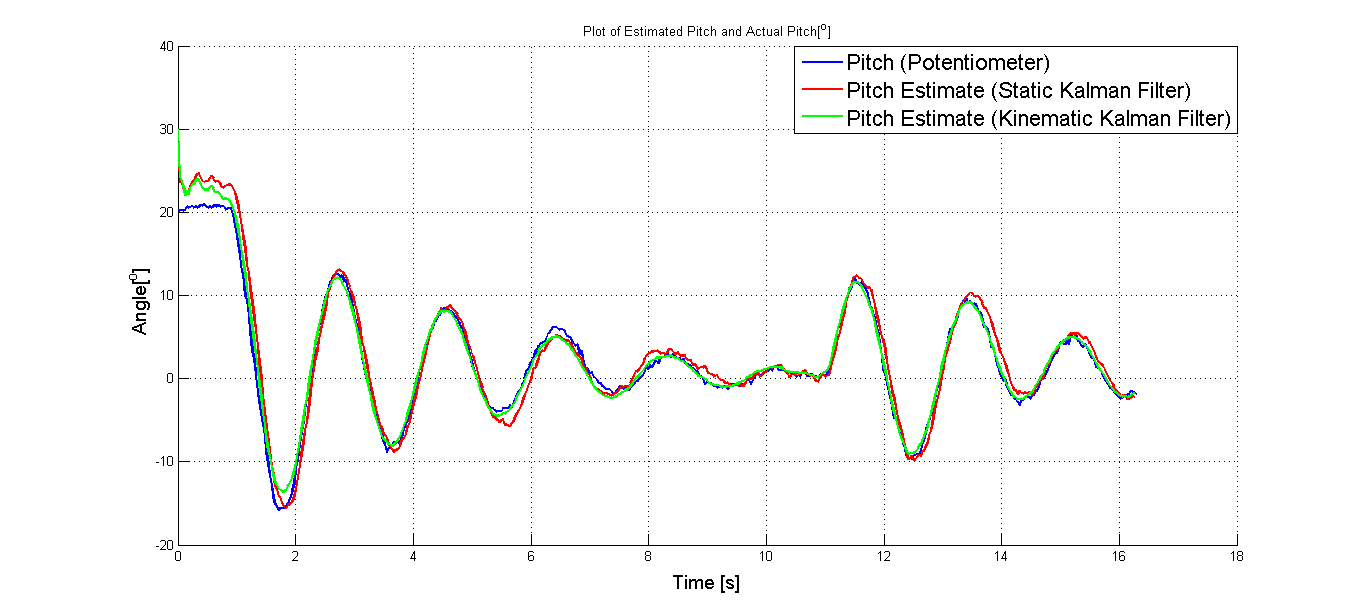
\includegraphics[width =0.36\paperwidth]{\DocRoot/images/Kalman_fitler_compare}
		\caption{Time domain comparison of Static and Kinematic Kalman Filter}
		\label{fg: Time domain comparison of Static and Kinematic Kalman Filter}
	\end{subfigure}%
	\hspace{3cm}
	\begin{subfigure}{0.32\textwidth}
		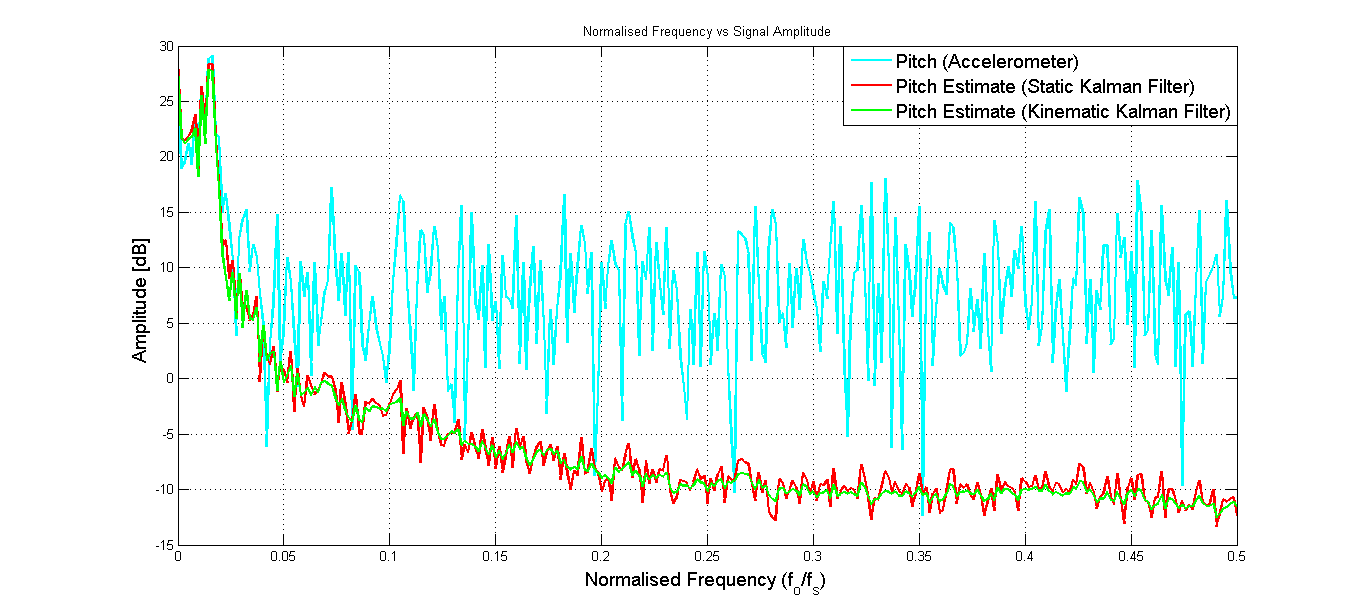
\includegraphics[width =0.36\paperwidth]{\DocRoot/images/fft_kalam_compare}
		\caption{Frequency domain comparison of Static and Kinematic Kalman Filter}
		\label{fg: Frequency domain comparison of Static and Kinematic Kalman Filter}
	\end{subfigure}

\caption{Comparison of Kalman Filters used during the Project}
\label{fig kalman filter comparison}	
\end{figure}

\section{Testing the Kalman Filter in Simulation}
To convert the Matrix Exponentiation function used in MatLab, approximations have to be made as the processing power required to calculate the Matrix Exponentiation in full is too great.

\subsection{Approximations Used}
So as to implement the Kinematic Kalman Filter on the micro-controller an approximation to the Matrix Exponential was made. The Matrix Exponential can be defined as follows:- 

\begin{equation}
e^{\underline{\bf X}} = \sum_{k=0}^{\infty}\frac{1}{k!}{\underline{\bf X}}^k
\label{eq: matrix exponential}
\end{equation}

Equation \ref{eq: matrix exponential} is an infinite series, thus, an approximation is required to implement the filter on the micro-controller.

\begin{equation}
e^{\gls{skewmatrix}\gls{ts}} = I + \gls{skewmatrix}\gls{ts} + \frac{(\gls{skewmatrix}\gls{ts})^2}{2!} + \dddot{}   +\frac{(\gls{skewmatrix}\gls{ts})^5}{5!}  
\end{equation}

It was not required to go beyond the $3^{th}$ term in the approximation of the matrix exponential since terms larger than the $3^{th}$ were of too small a magnitude to affect the result.



\section{Testing the Estimator with the Sensors}
Section \ref{sec: kalman filter responces} shows the Kalman Filters response in simulation. However, when estimating the orientation of the quad-rotor, the actual orientation was required to ensure the estimate produced by the filter was correct. This was achieved by placing the sensors on the quad-rotor, which in turn was mounted on a rig, which had potentiometers to measure the actual orientation. The rig was arranged so that the pitch and roll could not vary more than $\pm 30^o$. A picture of this arrangement can be seen in Figure \ref{Fig: test rig}. The \gls{noisecomatrix} was chosen by gathering data while the sensor was level and at rest. This data was called into MatLab where the \textit{cov} command was used to find the covariance of the accelerometer, gyroscope and magnetometer respectively. The \gls{noisecoplantmatrix} value for the Static Kalman Filter was difficult to acquire without flight data so it had to be approximated. As for the Kinematic Kalman Filter, the \gls{noisecoplantmatrix} was set to the covariance value of the gyroscope as the \gls{Transitionmatrix} of this filter is made from the gyroscope outputs. 


The code used to communicate with the \gls{9dof} was modified so that the potentiometer values could be read by means of an {ADC} on the micro-controller board. After the Micro-controller read the associated values (both \gls{9dof} values and potentiometer values) they were then recorded on a SD card so the data could be called into MatLab. This allowed post processing to be applied to the \gls{9dof} data. The \gls{noisecoplantmatrix} was adjusted until the potentiometer data matched the estimate produced by the Kalman Filter at both high and low accelerations.



\begin{figure}[h]
	\centering
	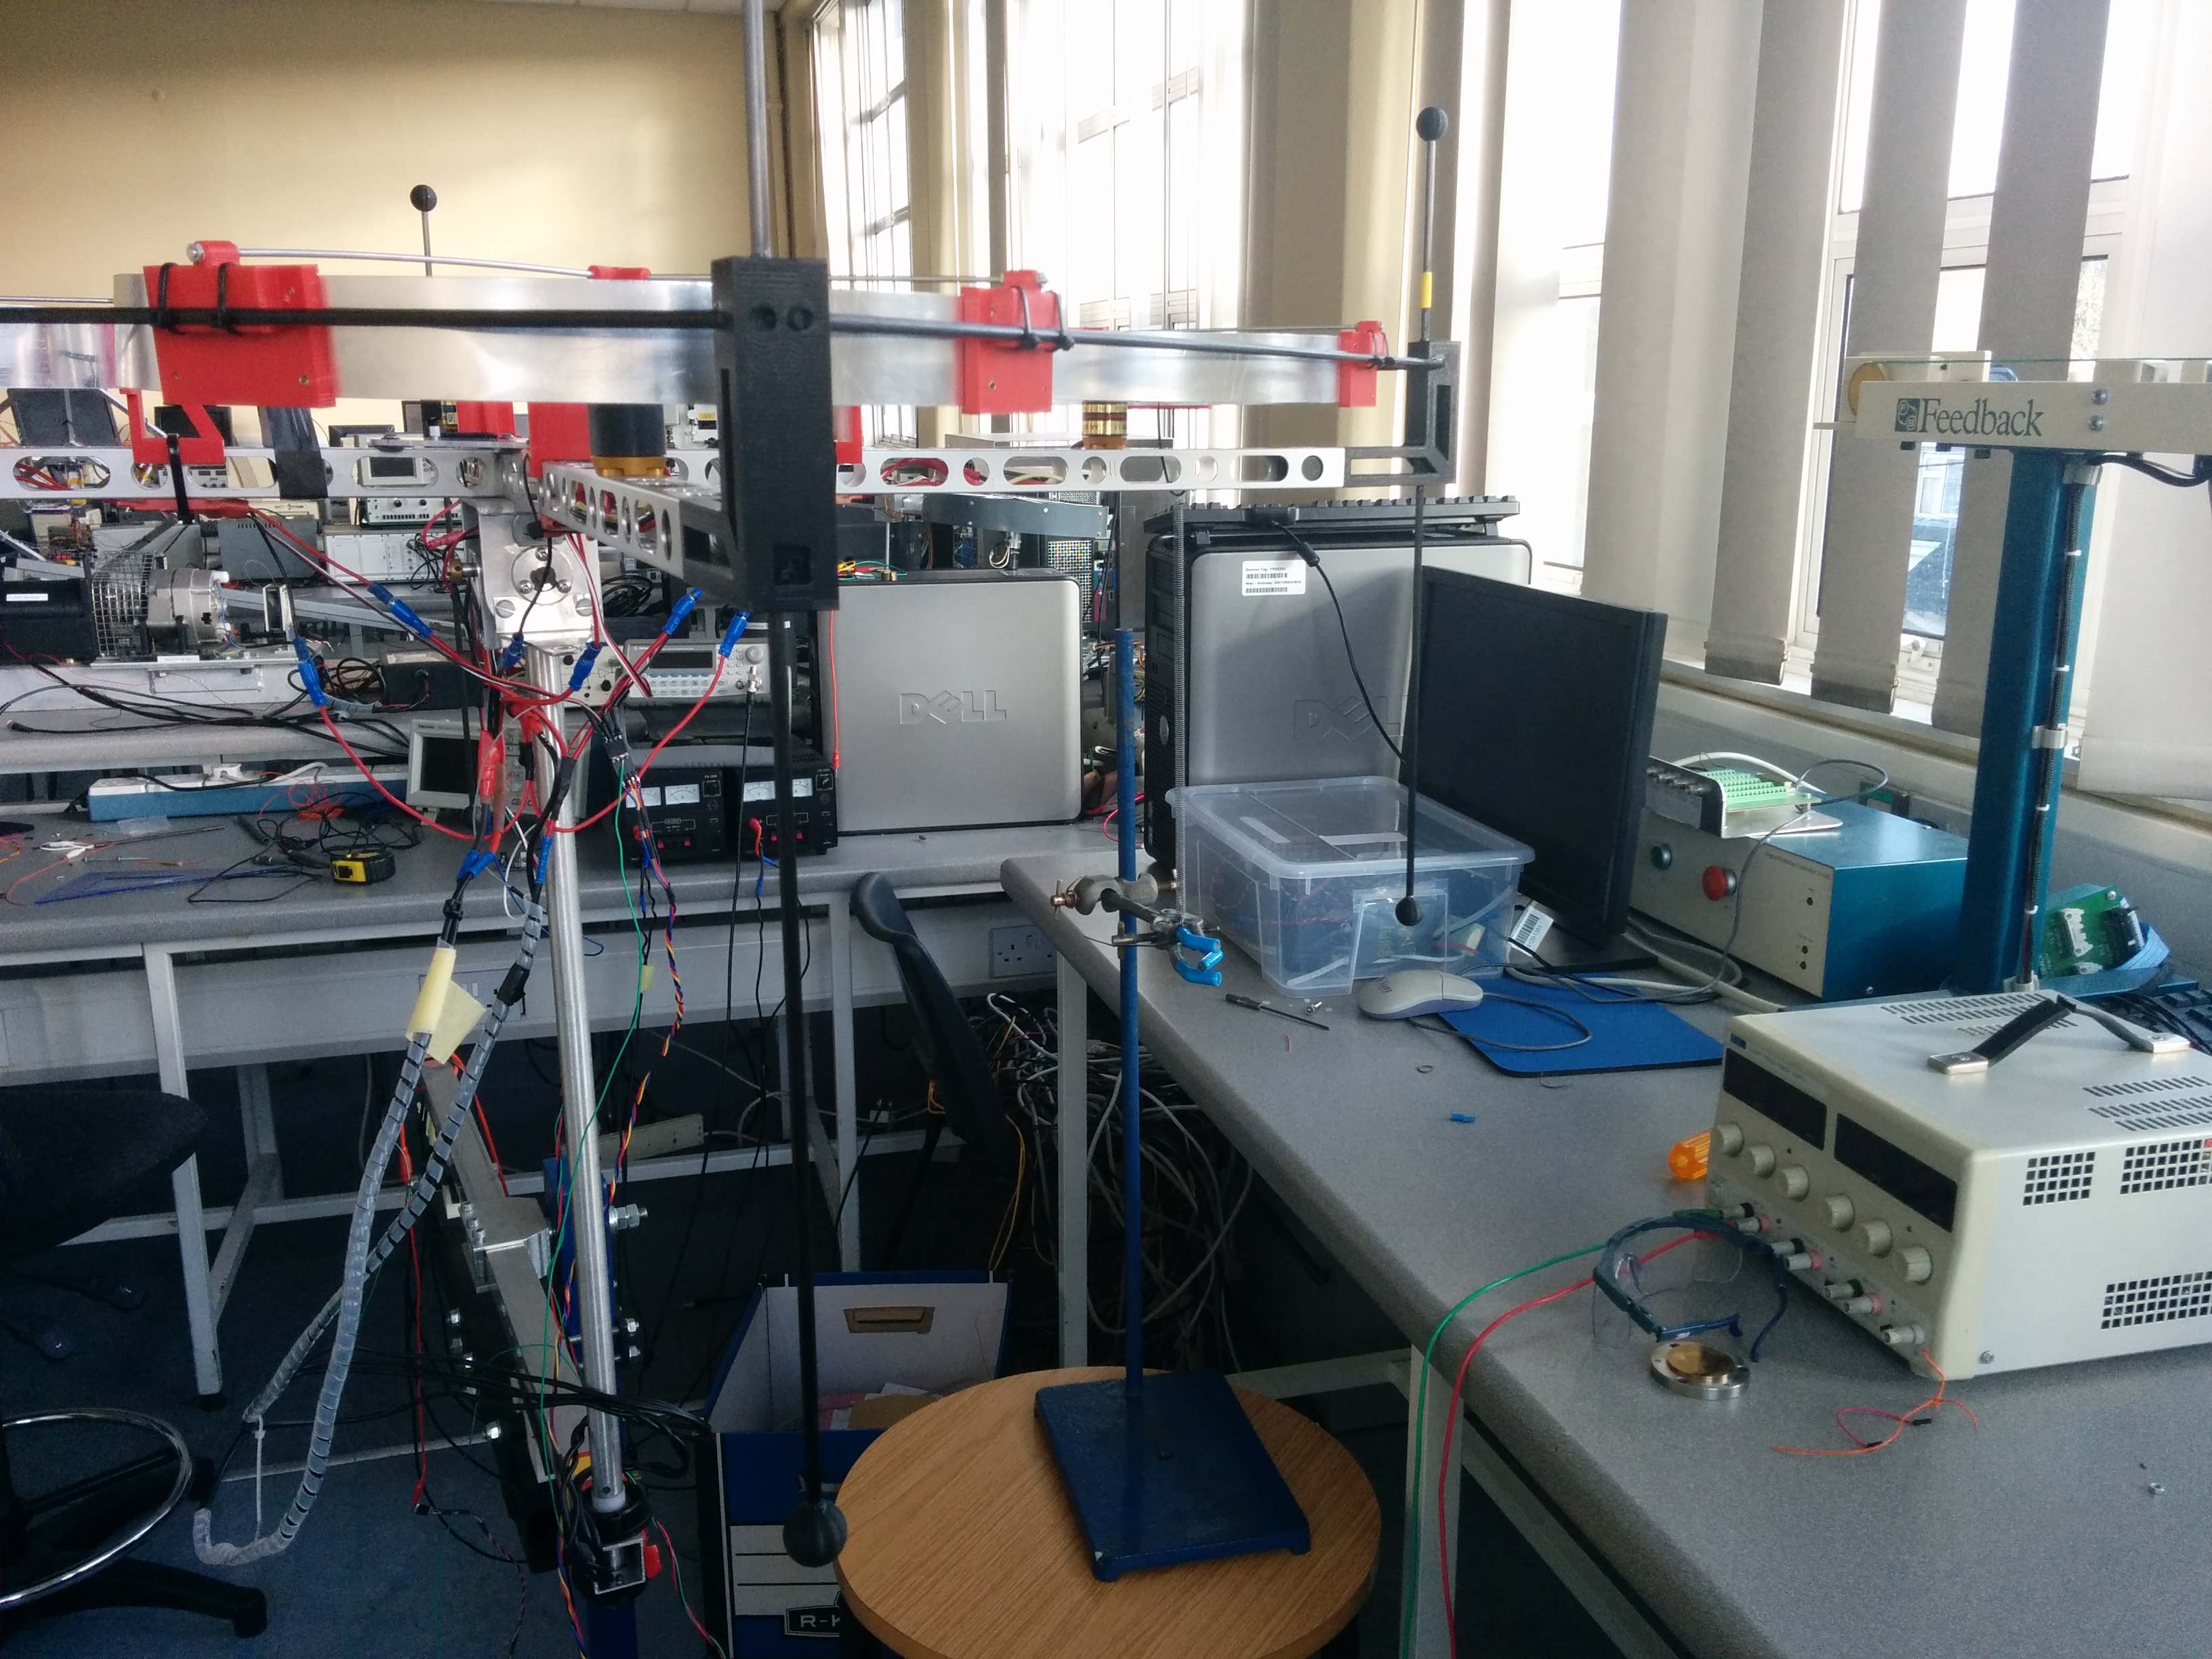
\includegraphics[width =0.7\paperwidth]{\DocRoot/images/quad_photo}
	\caption{Rig used to test the Kalman Filter}
	\label{Fig: test rig}
\end{figure}


\section{Tuning the Kalman Filter}
The Kalman Filter is often used as an estimator, but is widely known to be difficult to tune. Tuning the filter implies determining the \gls{noisecomatrix} and \gls{noisecoplantmatrix} matrices which control how the filter combines the model and the measurement to acquire an accurate estimate of the state vector. The accuracy of the filter's estimate depends on the \gls{noisecomatrix} and \gls{noisecoplantmatrix} matrices. Throughout the project many tuning methods were investigated, but the tuning method presented in \cite{gordon_paper} gave the best/desired results. The \gls{noisecomatrix} matrix can be estimated with ease, as the covariance of the data produced by the sensor while at rest can easily be found.

\subsubsection{Estimating the \gls{noisecomatrix} matrix}
As the accelerometer was thought to have a greater covariance at high accelerations (as the accelerometer also measures linear and angler acceleration) it was decided to test the device under high acceleration. In order to see if high acceleration components increased the covariance of the accelerometer data it was decided to gather data on the quad-rotor under high acceleration with motors on. It was found that the high acceleration components where lower than the noise floor produced by the vibrations due to the motors attached to the quad-rotor. The omission of the "high" high acceleration was possible as the magnitude of the angular acceleration of the quad-rotor is quite low. The covariance was found by means of the $cov()$ function in MatLab. Hence, the \gls{noisecomatrix} was calculated as follows:-

					\begin{equation}
					\gls{noisecomatrix}_a  = 		
					\left[\begin{array}{ccc}
					\mathrm{cov(\gls{roll})}       &                 0                          & 0\\ 
					0       & \mathrm{cov(\gls{pitch})}           & 0\\
					0         &                0                          &\mathrm{cov(\gls{yaw})}
					\end{array} \right]
					\end{equation}


\subsubsection{Estimating the \gls{noisecoplantmatrix} matrix}

 Calculating the \gls{noisecoplantmatrix} matrix proved to be quite a difficult task. Very little actual information regrading the noise present in the states was known. However, since \gls{noisecoplantmatrix} was difficult to calculate without flight data it was decided to use a binary search using the ratio of \gls{noisecoplantmatrix}/\gls{noisecomatrix} as it was shown in \cite{gordon_paper} that this type of tuning could lead to an optimal response. In this tuning process the \gls{noisecomatrix} was set to the theoretical value and \gls{noisecoplantmatrix} was adjusted by means of a binary search, thus a filter signal similar to the potentiometer value was found. A similar approach was used to tune the Kinematic Kalman Filter, except some initial knowledge was known about the \gls{noisecoplantmatrix} as the transition matrix of this filter was made up solely of the gyroscope values. This allowed the \gls{noisecoplantmatrix} matrix for this filter to be set to the covariance values of the gyroscope. This approach produced almost identical results to the Static Kalman Filter with little tuning, but in order to improve the filtering of the Kinematic Kalman Filter a binary search was also used to improve the estimation of this filter and the results of both Kalman Filters can be seen in figure \ref{fig kalman filter comparison}.                                                                                                                                                                                                                                                                                                                                                                                                                                                                                                                                                                                                                                                                                                                                                                                                                                                                                                                                                                                                                                                                                                                                                                                                          

\chapter{Optimal Controller Design}

\section{Optimal Control Design}
The previous sections develop methods of estimating the attitude of the quad-rotor by means of sensor fusion. The results from the Kalman Filter are used in developing a mathematical model of the quad-rotor and also as inputs to a controller and estimator. Figure \ref{Fig: Block Diagram of Final control of the Quad-Rotor} gives a block diagram comprising of the different sections required in the overall control of the quad-rotor.



\begin{figure}[h]
	\centering
	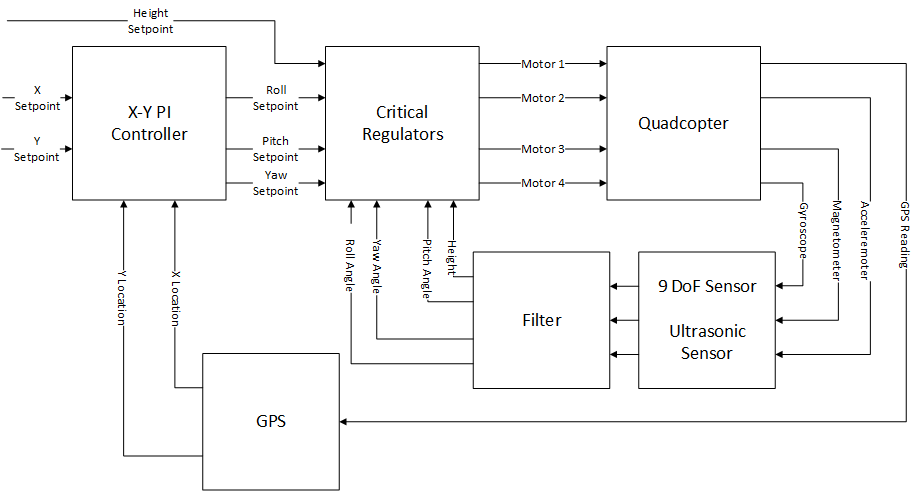
\includegraphics[width =0.7\paperwidth]{\DocRoot/images/Cascaded_Control}
	\caption{Block Diagram of Final control of the Quad-Rotor}
	\label{Fig: Block Diagram of Final control of the Quad-Rotor}
\end{figure}
The combination of gyroscopes and accelerometers are referred to as smart sensors, which estimates pitch, roll yaw and there respective rates.

The Kalman Filter and controller were designed and simulated using MatLab based on the quad-rotor model presented in \ref{eq: quad rotor model}. The current control set-points are roll,pitch and yaw, but the control has been developed for $x$ and $y$ to be made the set-points of the system. The current state used in the quad-rotor control scheme are as follows [$\gls{pitch},\gls{roll},\gls{yaw},\dot{\gls{pitch}},\dot{\gls{roll}},\dot{\gls{yaw}},h,\dot{h},\Delta\omega$]

\newpage
{
	\begin{description}[itemsep=1mm]
		\item[{\bf Where:-}]
		\item[\gls{pitch},\gls{roll},\gls{yaw}:] are the angle at which the quad-rotor is with respect to the $x,y$ and $z$ respectively.
		\item[$\dot{\gls{pitch}},\dot{\gls{roll}},\dot{\gls{yaw}}$:] are the rate of change of these angles
		\item[$h,\dot{h}$:] is the height and rate of change of height of the quad-rotor 
		\item[$\Delta\omega$:] is the differential thrust difference between the two opposing motors
		along an axis. 
	\end{description}
}

The type of controller designed to control the quad-rotor is an optimal controller, which controls the quad-rotor by selecting regulator gains for the best possible performance. To achieve this, the aspects of the plants behavior that are desired to be controlled must be incorporated in a mathematical expression referred to as the \enquote{cost function}. 

\section{Design of a \gls{lqr} Controller}
As the control scheme used on the quad-rotor was digital then any optimal controller used to stabilize the system had to be in discrete form too.Hence, the cost function to be minimized was of the discrete form and is defined as follows:- 

 \begin{equation}
 J_N  = \frac{1}{2} \sum_{n=0}^{N-1}(x_n^\intercal {\bf Q} x_n + u_n^\intercal {\bf R }u_n) + \frac{1}{2}x_N^\intercal {\bf Q}_N x_N
 \label{eq: discreter lqr}
 \end{equation}
 where $x$ and $u$ denote the states and inputs of the system respectively and {\bf Q} and {\bf R} are matrices chosen to apply the desired weights to various states and inputs respectively. 
 
 A controller designed by this approach is known as a \gls{dlqr} and is tuned by changing the ${\bf Q}$ and ${\bf R}$ matrices shown in \eqref{eq: discreter lqr} to give the optimal response. The ${\bf Q}$ and ${\bf R}$ matrices set a weighting on the state variable tracking and the control action respectively. If {\bf Q} is increased then a penalty is introduced which limits the deviation of the states from their set-points. Following from this if the {\bf Q} matrix is increase so too is the feedback gains. In contrast, if the {\bf R} matrix is increased, then aggressive control responses are penalized, which leads to a reduction in the feedback terms. Even though an \gls{lqr} controller is an optimal controller there are limitations inherent in its design. The main failing of an \gls{lqr} based control scheme is the fact that its frequency response rolls of at 20 dB per decade \cite[pg 584-617]{Artofcontrol}. Since the \gls{lqr} controller has such a poor frequency response it is often used injunction with a optimal filter such as the Kalman Filter so as to alleviate this problem.
 
 \subsection{Tuning of the {\gls{lqr}} controller}
 When a \gls{lqr} based control scheme is implemented there is two methods of tuning the controller, one is to set the {\bf Q} and very {\bf R} until the desired response is achieved. This form of tuning is possible as the \gls{lqr} controller is derived in a similar manner to Kalman Filter. Hence, a tuning approach similar to that used to tune the Kalman Filter in Chapter \ref{chap: kalman implem} can also be used to tune the \gls{lqr} controller. 
 
 The second approach is to use Bryson's Rule \cite{franklin2006feedback}. Bryson's Rule works by setting a maximum acceptable value of each state and then penalizes them accordingly. Bryson's Rule is commonly denoted as follows:-      
 
 \begin{align}
 \begin{split}
 Q_{ii} &= \frac{1}{(z_i^{max})^2}~~~~~~~~~~~~~~  i\in 1,2,\ddddot{}l\\
 R_{ii} &= \frac{1}{(u_j^{max})^2}~~~~~~~~~~~~~~        j\in 1,2,\ddddot{}m
 \end{split}
 \end{align}
 
 {	
 	\begin{description}[itemsep=1mm]
 		\item[Where:-]
 		\item[$z_i^{max}$:] is the maximum acceptable value of the $i$ state of the system 
 		\item[$u_i^{max}$:] is the maximum acceptable value of the $i$ input of the system.
 	\end{description}
 }
 
 which means the \gls{lqr} equation can be redefined as follows:-
 \begin{equation}
 J_N = \int_{0}^{\infty}\left(\sum_{i=1}^{l}Q_{ii}z_i(t)^2 + \sum_{j=1}^{m}R_{jj}u_{j}(t)^2\right)
 \end{equation}
 This method of tuning the \gls{lqr} controller was advantages as it allowed a limited to be set on states which in real life had limits and could saturate. An example of such a saturation is the angular velocity of the motors and the \gls{pwm} signal which also has an upper limit.  


\newpage
\subsection{Observer Design}
As the state space controller used on the quad-rotor required unmeasurable states, an observer is required to estimate these unknown states. An observer was designed which used sensor readings and the mathematical model of the quad-rotor presented in Section \ref{sec: quad-model} to estimate the unknown states.The observer required knowledge of the desired responses, which is achieved by the placement if its poles. A common method of designing an observer is by means of the Butterworth Constellation Technique, such an observer can easily be designed in MatLab by means of the \textit{place} function.

\subsubsection{Butherworth Constellation Technique}

\begin{figure}[h]
	\centering
	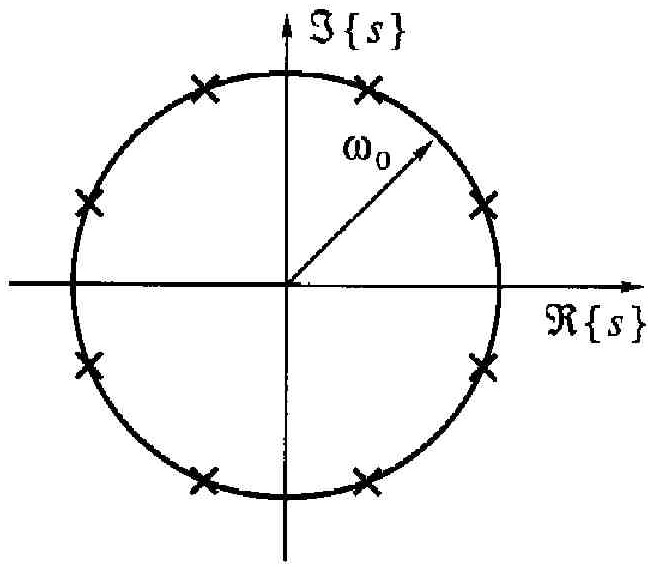
\includegraphics[width =0.4 \paperwidth]{\DocRoot/images/Butterworth_poles_2}
	\caption{8 Order Butterworth pole placement diagram }
	\label{Fig:butterworth diagram}
\end{figure}

Figure \ref{Fig:butterworth diagram} gives a graphical representation of the placing poles using the Butterworth Technique. The radius of the circle is $\omega_n$, found using the following:-

\begin{equation}
\frac{4}{\zeta \omega_n} = T_{s_{2\%}} \label{eq: observer design equation}
\end{equation}

 {	
 	\begin{description}[itemsep=1mm]
 		\item[Where:-]
 		\item[$\zeta$:] is the maximum acceptable value of the $i$ state of the system 
 		\item[$T_{s_2\%}$:] is the settling time of the observer.
 	\end{description}
 }

Once the observer was designed it was tested with the \gls{lqr} controller which was designed by means of \eqref{eq: discreter lqr}. The combination of the \gls{lqr} controller, observer and Kalman Filter the following response presented in Figure \ref{Fig:lqr controller}. Under this controller it was possible to control the roll,pitch and yaw axes.


\begin{figure}[h]
	\centering
	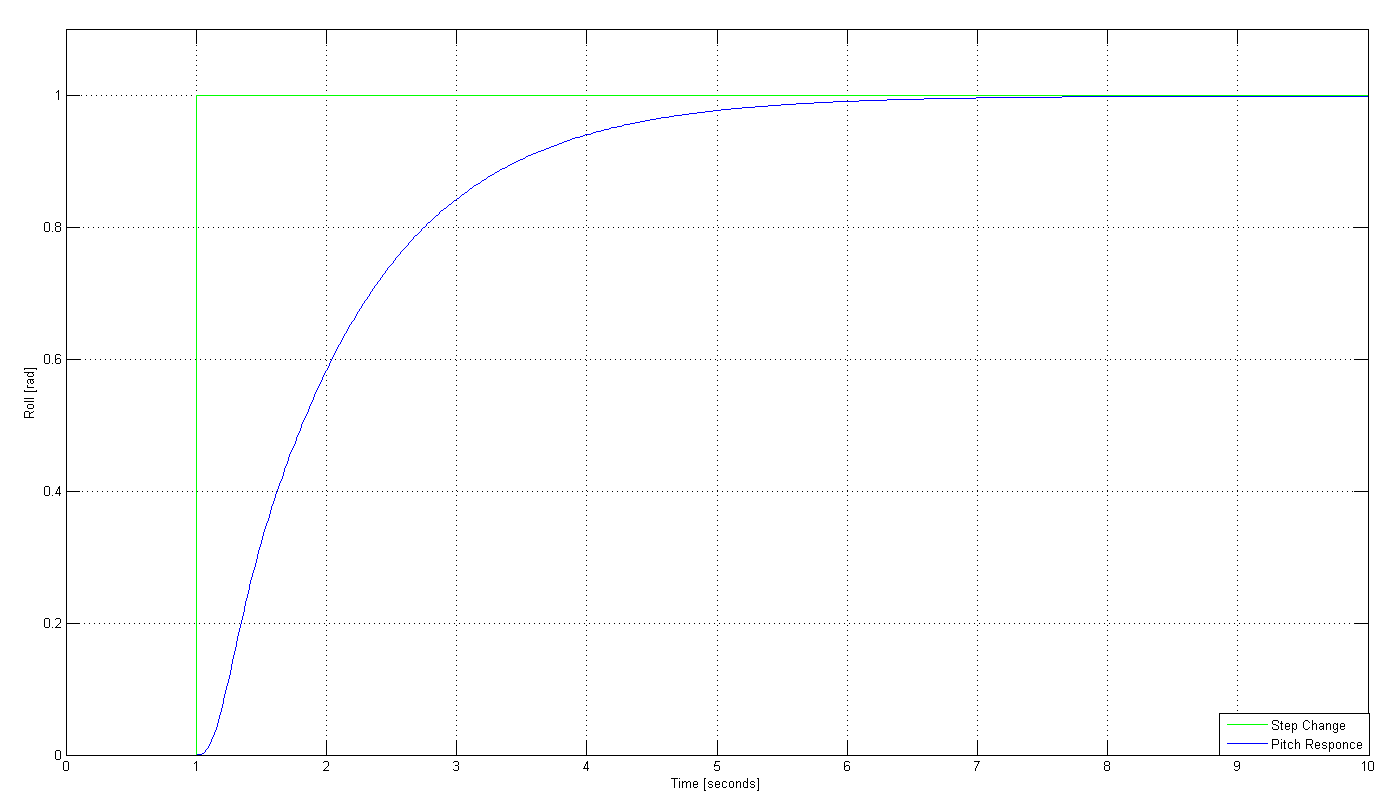
\includegraphics[width =0.6 \paperwidth]{\DocRoot/images/Roll_LQR1}
	\caption{Step response of the quad-rotor for the roll axis}
	\label{Fig:lqr controller}
\end{figure}

\chapter{Results}



This chapter discusses the results obtained when testing both the Complementary Filter and Kalman Filter. Initially the pitch angles were plotted over time with different \gls{noisecoplantmatrix} values until the best results was obtained. The estimated orientation from the Complementary Filter, Kalman Filter and the potentiometer data were plotted on the same graphs and compared.

\section{The Complementary Filter}
\subsection{The effect $\tau$ on Estimation}
The effect of $\tau$ on the estimate was tested by varying $\tau$ and can be seen in Figure \ref{fig effect of tau on filter}. Figure \ref{fig effect of tau on filter} compares the estimated data from the Complementary Filter with the actual values from the potentiometers. As seen in Figure \ref{fig effect of tau on filter} of the value of $\tau$ is set too low the accelerometer becomes the driving factor and the estimate remains noisy. While if $\tau$ is set too high the gyroscope data is used more than the accelerometer, hence a delay is introduced. Thus, a middle ground which will give an adequate estimate of the attitude of the quad-rotor. The best choice of $\tau$ was found to be 0.468 for use with this system. 


\begin{figure}[h]
	\centering
	\begin{subfigure}{0.32\textwidth}
		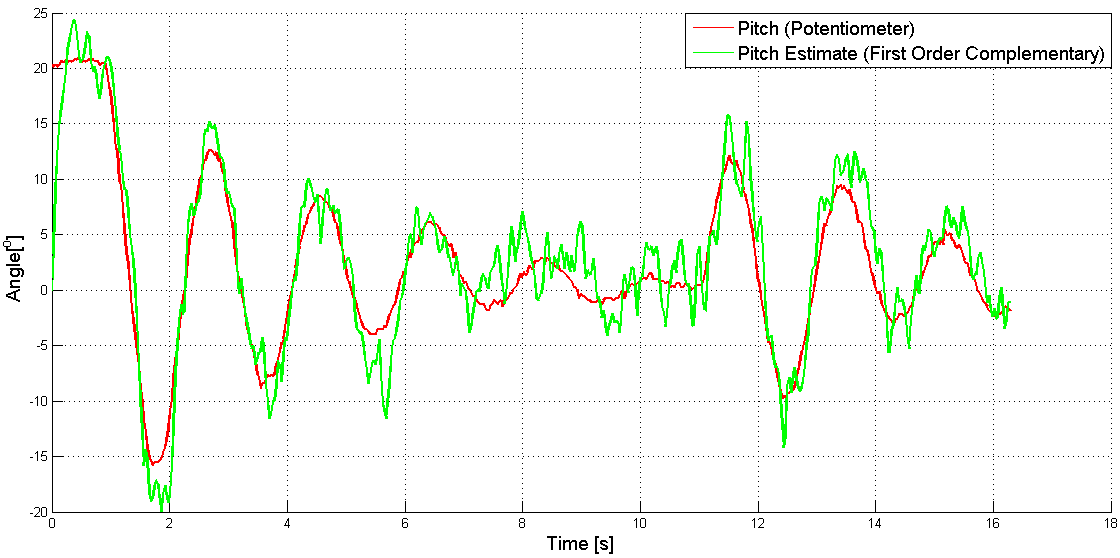
\includegraphics[width =0.38\paperwidth]{\DocRoot/images/comp_first_order_low}
		\caption{Pitch estimate with $\tau$ = 0.1}
		\label{Fig:low tau}
	\end{subfigure}%
	\hspace{3cm}
	\begin{subfigure}{0.32\textwidth}
		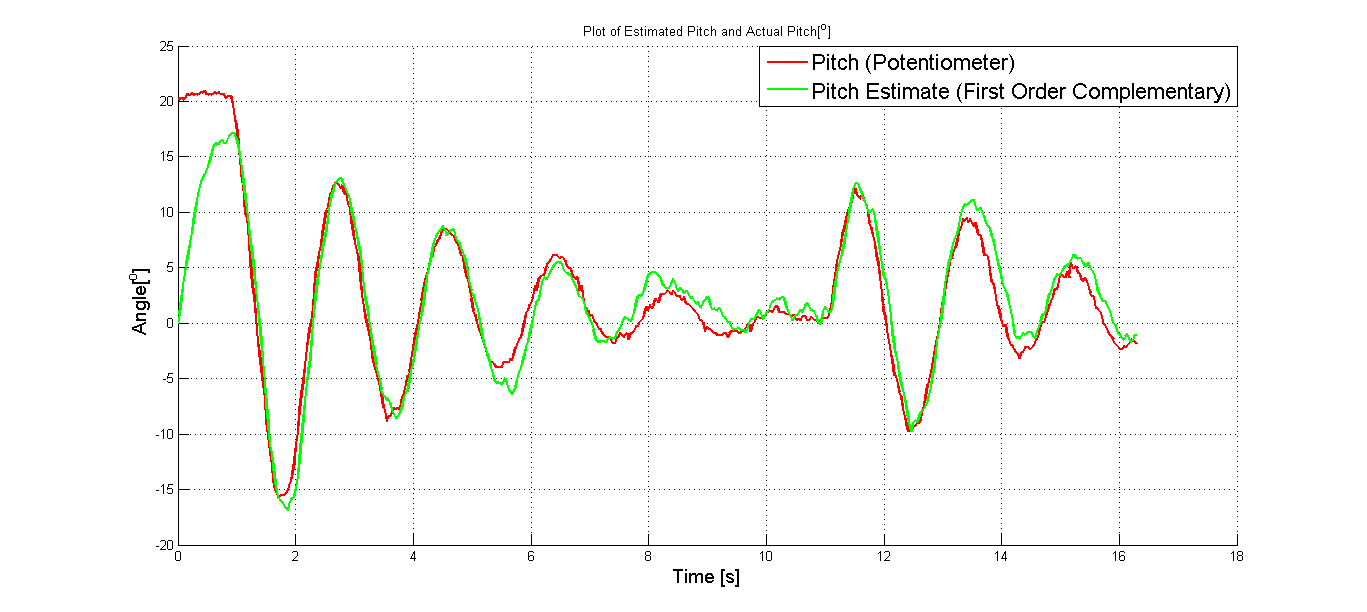
\includegraphics[width =0.38\paperwidth]{\DocRoot/images/comp_first_order_time}
		\caption{Pitch estimate with $\tau$ = 0.5}
		\label{Fig:high tau}
	\end{subfigure}
	\caption{Effect of varying $\tau$ on the estimate produced by the Complementary Filter}	
	\label{fig effect of tau on filter}
\end{figure}


\section{The Kalman Filter}
\subsection{Effect of Q on Estimation} 
The effect \gls{noisecoplantmatrix} has on the estimated was tested by varying the \gls{noisecoplantmatrix} matrix and comparing the estimated data from the Kalman Filter with the actual values from the potentiometers. In these tests, \gls{noisecomatrix} was kept constant at its theoretical value since it is the ratio of the two parameters that effect the estimate.


\begin{figure}[h]
	\centering
	\begin{subfigure}{0.32\textwidth}
		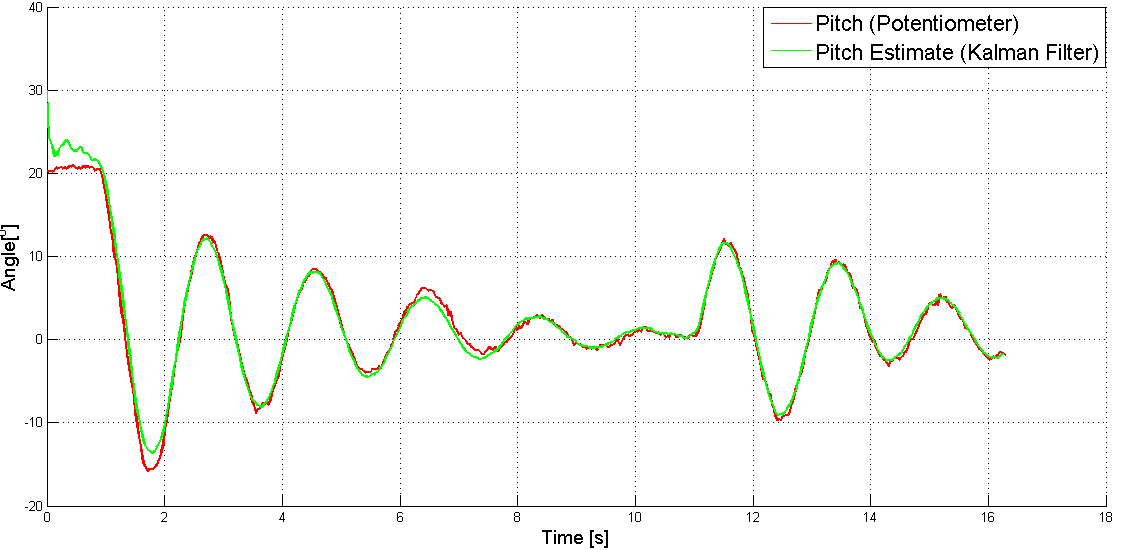
\includegraphics[width =0.38\paperwidth]{\DocRoot/images/Kalman_low}
	\caption{Pitch estimate with \gls{noisecoplantmatrix}/\gls{noisecomatrix} = $8.805\times10^{-5}$}
	\label{Fig:q/r ratio low}
	\end{subfigure}%
	\hspace{3cm}
	\begin{subfigure}{0.32\textwidth}
		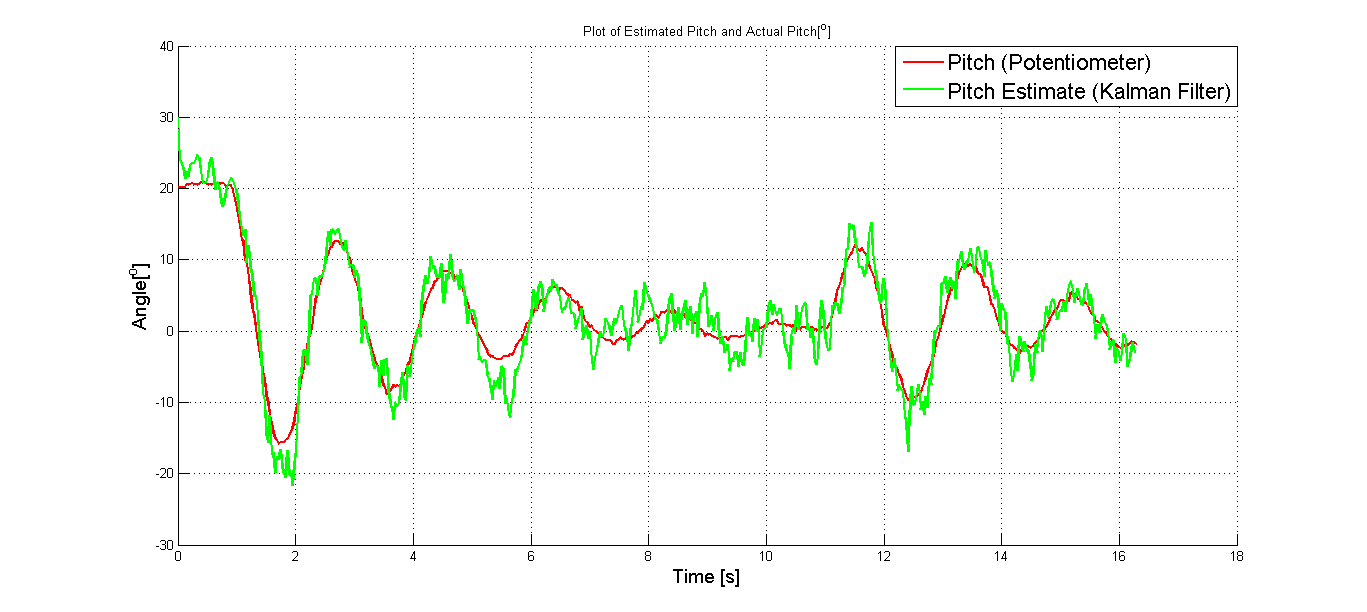
\includegraphics[width =0.38\paperwidth]{\DocRoot/images/Kalman_high}
	\caption{Pitch estimate with \gls{noisecoplantmatrix}/\gls{noisecomatrix} = 0.0881}
	\label{Fig:q/r ratio high}
	\end{subfigure}
	
	\caption{Effect of varying \gls{noisecoplantmatrix}/\gls{noisecomatrix} on the estimate produced by the Kalman Filter }	
\end{figure}
Figure \ref{Fig:q/r ratio low} and \ref{Fig:q/r ratio high} clearly show that the estimate of the pitch angles varies with \gls{noisecoplantmatrix}. At a lower \gls{noisecoplantmatrix} than \gls{noisecomatrix}, the response of the filter is more accurate. This implies that there is less noise on the states relative to the  measured signals. The Kalman Filter in this case assumes that the predicted pitch values are reliable and need little correction. Therefore increasing the Kalman gain matrix places more emphasis on the measurements and less on the prediction values \cite{gordon_paper}

Figure \ref{Fig:Cross-Correlation of estimated pitch error} shows the cross-correlation of the error between the estimated and actual pitch values. If the noise present in the Kalman Filter's model and the present in the accelerometer and gyros is Gaussian and uncorrelated, Figure \ref{Fig:Cross-Correlation of estimated pitch error} would be all zero except at the center, where the response would be one. Therefore, Figure \ref{Fig:Cross-Correlation of estimated pitch error} shows that the noise present in the signals is not uncorrelated.

\begin{figure}[h]
	\centering
	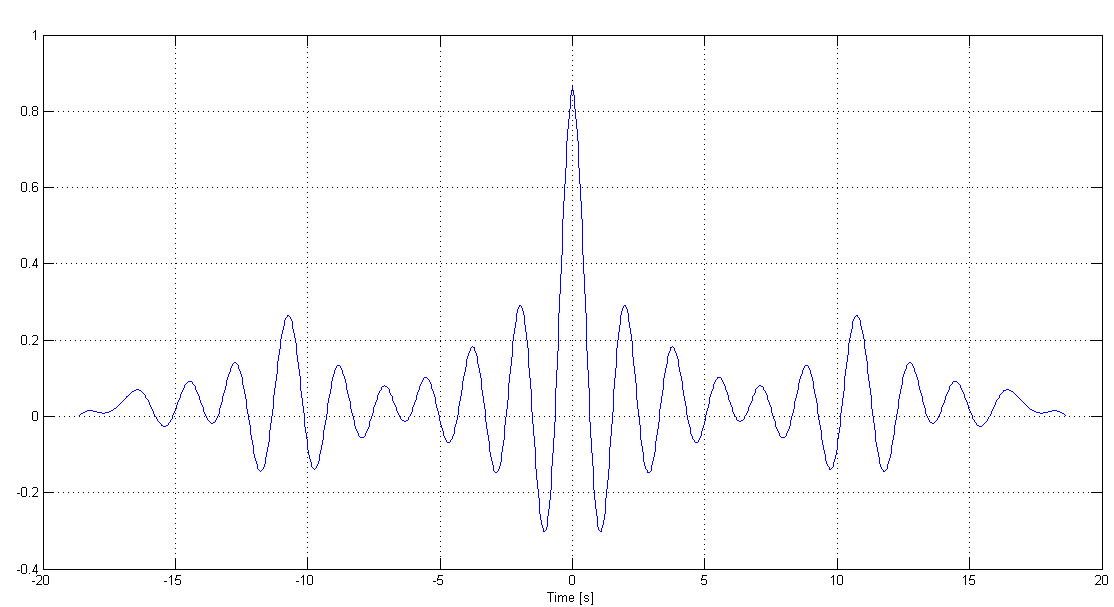
\includegraphics[width =0.8 \paperwidth]{\DocRoot/images/corelation_matlab}
	\caption{Cross-Correlation of estimated pitch error}
	\label{Fig:Cross-Correlation of estimated pitch error}
\end{figure}
\chapter{Future Work}

To-date the critical controllers have been designed, with the roll,pitch and yaw  having been tested on the quad-rotor. Also an $xy$ controller has been designed and the maths required to map \gls{gps} data to \gls{ned} frame where the positional control is implemented has been developed in this report. But as flight data was not collected a Kalman Filter was not implemented to convert the \gls{gps} data to the \gls{ned} frame were the control is implemented. Hence, the next action would be to collect flight data and find \gls{noisecomatrix} and \gls{noisecoplantmatrix} matrices for a \gls{gps} Kalman Filter. In the development of such a filter it maybe required to increase the up-date rate to the positional controller of the quad-rotor by doing more predict stages in the Kalman Filter and then correcting these \enquote{prediction} every $n$ cycles of the Kalman Filter by means of a correction up-date from the \gls{gps} module.  

After the Kalman Filter is developed, the quad-rotor would be semi/fully autonomous. As the \gls{gps} only gives accurate position while having access to four satellites, it might be beneficial to attach a vision system to the quad-rotor so the positional controller will have updates while the \gls{gps} link is broken. Also if a vision system is added to the quad-rotor, it would be possible to fly the quad-rotor in locations where \gls{gps} guidance is not possible, such as indoors.  

If the quad-rotor was capable of flying indoors, then building mapping could be a natural next step. This mapping could be done in two possible ways, by means of Lidar or ultrasonic sensors. The Lidar would be more expensive, but is more accurate, is less prone to interference and has a faster update. The ultrasonic sensors on the order hand are cheaper and require less power, but are less accurate and have a limited of operation.

  





\chapter{Conclusion}

A mathematical mode of the quad-rotor has be developed. Models for the accelerometer, gyroscope and magnetometer have been developed (as seen in  Section \ref{sec:imu section for relation of stuff})and proven to be correct by means of experiment. A \gls{gps} model has also been presented in Section \ref{sec: gps part} and can be used in future projects if a \gls{gps}-based device is used.


As the sensors used in the project are not ideal, the attitude of the quad-rotor had to be estimated by means of data fusion. These estimators have been tested in both simulation and on the quad-rotor.

The pitch and roll estimates were compared with actual values and the results showed that the filters worked as required an indeed produced an optimal response. Chapter \ref{chap: kalman implem} shows that the Kalman Filter is the optimal choice, but is more computationally intensive to run on some micro-controllers than a Complementary Filter. If the Kalman Filter is not an option, then a Complementary Filter similar to the ones presented in this report can be used for attitude estimate as they are less computational intensive.


The attitude estimators were designed and simulated using Simulink and MatLab. The results showed from these simulations demonstrated that these estimators could be implemented to control the quad-rotor. The Complementary Filter and Kalman Filer where both tested on the quad-rotor with a \gls{lqr} based control scheme and both were shown to give adequate  results.

Finally, the report gives a detailed description of how the filters compare to each other and how they can be implemented on a micro-controller. 




\begin{appendices}
    	\chapter{Modeling parameters}
	

	\begin{table}[h]
		\centering
		\begin{tabular}{|c||c|c|c|}
			\hline
			\multicolumn{1}{|c|}{}                                     & \multicolumn{1}{c|}{Parameter} & \multicolumn{1}{c|}{Value} & Unit            \\ \hline\hline
			\multicolumn{1}{|c||}{\multirow{5}{*}{Brushless DC motors}} & \gls{timeconstants}               & 0.07                       & s               \\ \cline{2-4} 
			\multicolumn{1}{|c||}{}                                     & \gls{inertiaofmotor}                      & 80                         & $\mathrm{\ensuremath{n}~kg~m^{2}}$    \\ \cline{2-4} 
			\multicolumn{1}{|c||}{}                                     &\gls{dragcoofmotor}                       & 0.44531                 & $\mathrm{\mu~kg~m^2~rad^{-}}$ \\ \cline{2-4} 
			\multicolumn{1}{|c||}{}                                     & \gls{trustcoofmotor}                           								 & 0.0189209                     &                 \\ \cline{2-4} 
			\multicolumn{1}{|c||}{}                                     & \gls{Motorcontant}                               							& 501.5133                   &   $\mathrm{rad}~s^{-2}$         \\\hline
			\multirow{12}{*}{Mechanical}                       & \gls{systemmass}                         	  & 2.26                       & Kg              \\ \cline{2-4} 
			                                                                                        &\gls{lenghtfromcenterofmass}    & 0.338                      & m               \\ \cline{2-4} 
			                                                                                        
			&\gls{interiaofroll}                     & 0.1274                     & $\mathrm{kg~m^{2}}$      \\ \cline{2-4} 
			& \gls{interiaofpitch}                & 0.1221                     & $\mathrm{kg~m^{2}}$      \\ \cline{2-4} 
			& \gls{interiaofyaw}                 & 0.237                      & $\mathrm{kg~m^{2}}$      \\ \cline{2-4} 
			& \gls{dampingroll}                  & 0.0194                     & $\mathrm{N~m~s^{-}}$     \\ \cline{2-4} 
			& \gls{dampingpitch}               & 0.0194                     & $\mathrm{N~m~s^{-}}$     \\ \cline{2-4} 
			& \gls{dampingyaw}                & 0                          & $\mathrm{N~m~s^{-}}$     \\ \cline{2-4} 
			& \ensuremath{g}                                     & 9.81                       & m $\mathrm{s^{-2}}$      \\ \cline{2-4} 
			& Total thrust                             & 32                         & N               \\   \cline{2-4} 
		   & damping in x                              & 32                         & $\mathrm{N~m~s^{-}}$              \\   \cline{2-4} 
			& damping in y                            &								&	$\mathrm{N~m~s^{-}}$ 				  \\  \hline
			Controller                                                 & \gls{ts}                             & 20                         & $\mathrm{m~s}$           \\ \hline
			\multirow{2}{*}{\gls{esc}}                                     &$ \gls{pwm}_{max}$                      & 2                          & $\mathrm{m~s}$           \\ \cline{2-4} 
			& $\gls{pwm}_{min}$                      & 0.9                        & $\mathrm{m~s}$           \\ \hline
		\end{tabular}
		\caption{Table of Essential Quad-Rotor Parameters}
	\end{table}
	
	
    \chapter{Rotation Matrix} \label{chap: Rotation Matrix reation}
\section{Derivation of the Rotation Matrix}


\pgfmathsetmacro{\rframe}{1.5}
\pgfmathsetmacro{\thetavec}{55}
\pgfmathsetmacro{\phivec}{35}
\pgfmathsetmacro{\framelengthy}{0.15}



\pgfmathsetmacro{\endpointx}{2.5}
\pgfmathsetmacro{\endpointy}{7}
\pgfmathsetmacro{\endpointz}{1.5}

	\begin{figure}[h!]
		\centering
	\begin{tikzpicture}[scale=5,tdplot_main_coords]
					\tdplotsetcoord{P}{\rvec}{\thetavec}{\phivec}
					\tdplotsetcoord{Px}{0.55}{90}{\phivec}
					\coordinate (O) at (0,0,0);
					
					
					\draw[thick,->] (0,0,0) -- (\framelengthsxy,-\framelengthy,0) node[anchor=north east]{$x_n$};
					\draw[thick,->] (0,0,0) -- (0,\framelengthsxy,0) node[anchor=north west]{$y_n$};
					\draw[thick,->] (0,0,0) -- (0,0,\framelengthsxy) node[anchor=south]{$z_n$};
					
								
					
					% NED Frame 
					\tdplotsetrotatedcoords{\phivec}{\thetavec}{0}
					\tdplotsetcoord{Q}{\rframe}{\thetavec}{\phivec}
					\tdplotsetrotatedcoordsorigin{(Q)}
					%\draw[dashed,tdplot_rotated_coords,-,draw=green,fill=white] (-0.1,-0.1,0)
					-- (-0.1,0.1,0) -- (0.1,0.1,0)  -- (0.1,-0.1,0)  -- cycle  ;
					\draw[thick,tdplot_rotated_coords,->,black] (0,0,0)
					-- (-\framelengthsxy+0.02,0,0) node[thick,left]{$y_b$};
					\draw[thick,tdplot_rotated_coords,->,black] (0,0,0)
					-- (0.0,\framelengthsxy,0) node[thick,below]{$x_b$};
					\draw[thick,tdplot_rotated_coords,->,black] (0,0,0)
					-- (0,0,\framelengthz) node[thick,above]{$z_b$};
					
					
			  
				\tdplotsetcoord {end}{\rvec+\endpointx}{\thetavec+\endpointy}{\phivec+\endpointz}
				\draw node at (end) [joint] (joint2) {};
				\draw[thick,dashed,->](O) -- node[above]{${\bf \footnotesize P}$}(Q);
				%\draw[->](Q) -- node {$P$}(end);
				\draw[thick,dashed,->](Q) -- node[above]{${\footnotesize{\bf \xi^B}}$}(joint2);
				\draw[thick,dashed,->](O) -- node[below]{${\footnotesize{\bf \xi^N}}$}(joint2);
			\end{tikzpicture}
		\caption{General Transform of a Vector}
		\label{fig: General Transform of a Vector}
	\end{figure}
	
	The unit vector $x_b,y_b,z_b$ define the (B) frame. In terms of the corresponding vectors of frame (N) these unit direction vectors become $x_b^n,y_b^n,z_b^n$,where
	
	\begin{equation}
	x_b^n = \begin{bmatrix}
	       x_b.x_n\\
	       x_b.y_n\\
	       x_b.z_n
	\end{bmatrix}
	\end{equation}
	Thus, the orientation of frame (B) with respect to frame (N) can br defined as $3x3$ matrix.
	
	\begin{equation}
	R_N^B = [x_b^n,y_b^n,z_b^n]
	\label{eq:rotation matrix derivation}
	\end{equation}
	
	The matrix presented in \ref{eq:rotation matrix derivation} is referred to as a rotation matrix. It  is equal to the rotation that must be applied to (N) to place it at (B)
	
	Hence, from figure \ref{fig: General Transform of a Vector} on can define the following equation:-
	
	\begin{equation}
	\xi^N = R_N^B\xi^B + P
	\label{eq: roatation intermeate}
	\end{equation} 
	
	Manipulating \eqref{eq: roatation intermeate} and using the property $(R^B_N)^{-1}$ = $R_B^N$ = \gls{rotationmatrix},
	\begin{equation}
	\zeta^B = \gls{rotationmatrix}(\zeta^N-P)
	\end{equation}
	
	\subsection{Euler Angle Derivation} 
	
	As \eqref{eq:rotation matrix derivation} has been already defined, it is now possible to define any 3-D vector mapping using the following \footnote{This is commonly refereed to as the general case of for the Euler Angle Relationship} :-
	
	\begin{equation}
	R^B_N =R^{B'}_N R^{B''}_{B'} R^{B'''}_{B''} 
	\end{equation}
	
	These relationship was used to find the rotation matrix presented in \ref{sec: euler angles}.
\subsection{Proof of the Transition Matrix used in Kinematic Kalman Filter}

\begin{align}
\begin{split}
\dot{x} &= \gls{skewmatrix}x\\
\int_{x_{k+1}}^{x_{k}}\frac{1}{x}dx &= \int_{k + \gls{ts}}^{k}\gls{skewmatrix}dt\\
\ln\left|\frac{x_{k+1}}{x_{k}}\right| &= \gls{skewmatrix}\gls{ts}\\
x_{k+1} &= e^{\gls{skewmatrix}\gls{ts}}x_k = \gls{Transitionmatrix}_kx_k
\end{split}
\label{eq:kalman matrix exp proof}
\end{align}

\eqref{eq:kalman matrix exp proof} uses the matrix exponential to find the transition matrix at each iteration. In other to implement this on a micro-controller \eqref{eq: matrix exponential app} can be truncated \footnote{In this project it was found that 5 terms where sufficient to capture the required information of the matrix exponential} to a set number of terms, which would all \eqref{eq:kalman matrix exp proof} to be implemented on a micro-controller at each up-data of the kinematic Kalman Filter.

\begin{equation}
e^{\underline{\bf X}} = \sum_{k=0}^{\infty}\frac{1}{k!}{\underline{\bf X}}^k
\label{eq: matrix exponential app}
\end{equation}
    	\chapter{Definition of Statistics used in the Implementation of the Kalman Filter} \label{chap: statist stuff for kaman}
	\section{Mean}
	The mean or average value of a time-varying signal $x(t)$ can be found by taking a total of $N$ measurements of $x(t)$ at regular intervals. Hence, the mean can then be found by means of \eqref{eq: mean} 
	
	\begin{equation}
	\bar{x} = \frac{1}{N}\sum_{k=1}^{N}x_k
	\label{eq: mean}
	\end{equation}
Note the mean is also stated/known as the expected value, which is denoted $E[x]$. Therefore $E[x] = \bar{x}$.

\section{Standard Deviation}

The standard deviation is a statistic that gives an indication into how tightly all the measurements $x(t)$ are clustered around the mean value in a set of data. It is found by calculating the root-mean-square of the deviations of the samples from the mean and is defined as follows :-

\begin{equation}
\sigma_x = \sqrt{\frac{1}{N} \sum_{k=1}^{N} (x_k - \bar{x})^2}
\end{equation}   	
	
	
	\section{Variance}
	The variance of a set of data provides information about how far samples of $x(t)$ are spread around/from the expected value. If the variance is high, it implies the data has a wide spread around the "mean" and vice versa. The  unbiased sample variance is calculated using the following :-
	
	
	\begin{equation}
	\sigma_x^2 = \frac{1}{N-1} \sum_{k=1}^{N} (x_k - \bar{x})^2
	\end{equation}   	
	Note the variance can also be denoted as $ \sigma_x^2 = E[(x-\bar{x})^2]$
	
	
	\section{Covariance}
	The covariance is a measure of how much two random variables change together and how strongly they relate. Taking two zero-mean signal $x(t)$ and $y(t)$, the covariance between them can be found using the following.
	
	\begin{equation}
	\sigma(x,y) = \frac{1}{N-1}\sum_{k=1}^{N}(x_i - \bar{x})(y_i-\bar{y}) = E[(x - \bar{x})(y - \bar{y})] 
	\end{equation} 
	

	
	Hence, if $x(t)$ and $y(t)$
are uncorrelated signal, then $\sigma_{xy} = 0$ \footnote{The Covariance of a signal $x(t)$ and $y(t)$ is most commonly denoted $\sigma_{xy}$}

\section{The Covariance Matrix}

Taking signal vector, $\underline{\bf x} (t)$, made up of $n$ random signals [$x_1,x_2,\ddddot{},x_n$], the covariance matrix contains all possible covariances between elements of the vector, resulting in the following:-
\begin{equation}
\sigma^2(\underline{\bf x} )=\left[\begin{array}{cccc}
\sigma^2_{x_1} &\sigma_{x_1}\sigma_{x_2} &\dots& \sigma_{x_1}\sigma_{x_n}\\
\sigma_{x_2}\sigma_{x_1} &\sigma^2_{x_2} &\dots& \sigma_{x_2}\sigma_{x_n}\\
\vdots& \vdots& \ddots &\vdots\\
\sigma_{x_n}\sigma_{x_1} &\sigma_{x_n}\sigma_{x_2} &\dots&\sigma^2_{x_n} \\
\end{array}\right] \label{eq: Covariance matrix}
\end{equation}	

Due to the commutative property of the covariance between two signals, a covariance matrix is equal to is transpose. Also, if each data random signal above were independent of all other signals, the covariance matrix would be diagonal (i.e, all non-diagonal elements could be set to zero.) \footnote{Note \eqref{eq: Covariance matrix} is commonly written as $E[{\bf \underline{x}}{\bf \underline{x}}^\intercal]$}
\newpage

\section{Gaussian Variables}
Gaussian distribution is a measure of the probability density function of a time-varying signal. The graph of the probabilities of the data plotted against the amplitude of the probability density function results in a bell-shaped curve as shown in figure \ref{fig: gaussian dis}



\pgfmathdeclarefunction{gauss}{3}{%
	\pgfmathparse{1/(#3*sqrt(2*pi))*exp(-((#1-#2)^2)/(2*#3^2))}%
}

\begin{figure}[h]
	\centering
	\begin{tikzpicture}
\begin{axis}[
no markers, 
domain=0:6, 
samples=100,
ymin=0,
axis lines*=left, 
xlabel=$x$,
every axis y label/.style={at=(current axis.above origin),anchor=south},
every axis x label/.style={at=(current axis.right of origin),anchor=west},
height=5cm, 
width=12cm,
xtick=\empty, 
ytick=\empty,
enlargelimits=false, 
clip=false, 
axis on top,
grid = major,
hide y axis
]

\addplot [very thick,cyan!50!black] {gauss(x, 3, 1)};

\pgfmathsetmacro\valueA{gauss(1,3,1)}
\pgfmathsetmacro\valueB{gauss(2,3,1)}
\draw [gray,dashed] (axis cs:1,0) -- (axis cs:1,\valueA)
(axis cs:5,0) -- (axis cs:5,\valueA);
\draw [gray,dashed] (axis cs:2,0) -- (axis cs:2,\valueB)
(axis cs:4,0) -- (axis cs:4,\valueB);
\draw [yshift=1.4cm, latex-latex](axis cs:2, 0) -- node [fill=white] {$0.683$} (axis cs:4, 0);
\draw [yshift=0.3cm, latex-latex](axis cs:1, 0) -- node [fill=white] {$0.954$} (axis cs:5, 0);

\node[below] at (axis cs:1, 0)  {$\bar{x} - 2\sigma$}; 
\node[below] at (axis cs:2, 0)  {$\bar{x} - \sigma$}; 
\node[below] at (axis cs:3, 0)  {$\bar{x}$}; 
us\end{axis}
\end{tikzpicture}
\caption{Gaussian Distribution of a time-varying signal}
\label{fig: gaussian dis}
\end{figure}


Note the Gaussian distribution can be represented by \eqref{eq: gaussian dis} 

\begin{equation}
f(x,\bar{x},\sigma) = \frac{1}{\sigma \sqrt{2\pi}}e^{-\frac{(x-\bar{x})}{2\sigma^2}}
\label{eq: gaussian dis}
\end{equation}  

\section{White Noise}
White noise can be considered as noise that contains all the possible frequency components at equal probability. It therefore has a flat probability distribution when plotted against frequency. However, it's Gaussian in terms of the amplitude of the noise. The spectral density function of white noise can be seen figure \ref{fig: white noise}
	
	\begin{figure}[h]
		\centering
		\begin{tikzpicture}
\draw node at (0,-0.5){0}  ; 		
\draw[->][line width=1.0pt] (-4.5,0) -- (4.5,0) node[anchor=north west] {\ensuremath{\omega}};
\draw[->][line width=0.5pt] (0,0) -- (0,4.5) node[anchor=south east] {\ensuremath{S(j\omega)}};
\draw[line width=1.7pt] (-4.5,2) -- (4.5,2) {};
		\end{tikzpicture}
		\caption{Spectral density function of white noise}
		\label{fig: white noise}
	\end{figure}
    \chapter{Kalman Filter}
This appendix draws heavily on the work present in \cite{bin}. As stated in the main report the Kalman Filter is a recursive filter which computes corrections to a system based on external measurements. The amount at which the filter corrects the values depends on the current estimate of the system error statistics. Note the filter requires knowledge of linear algebra and stochastic processes. As the filter requires knowledge of stochastic processes it can be quite difficult to understand, fortunately, it can be understood in fairly simple terms. All that is required is an understanding of various common statistical properties, which are presented in Appendix \ref{chap: statist stuff for kaman}

Before the Kalman Filter is introduced the concept of a state vector must be defined as it is central to the formulation of the filters algorithm. A state vector is a set of values which are used to describe the \enquote{state} of the system. For this project, which is a navigation system, the state vector is given as position,velocity,attitude and sensor errors. Since the filter is used to correct errors in a navigation system, working in terms of error states is convenient and for an arbitrary state $x$, the estimate can be defined as follows:-   

\begin{equation}
\hat{x} = x + \delta x
\end{equation} 

where $x$ is the true value of the state and $\delta x$ is the error in the estimate. The purpose of the Kalman Filter is to estimate this error $\delta x$ and correct it.

In order to derive such a filter all system equations and measurement equations have to be expanded in a Talyor series. As the error in the states are small, it is only required to keep the first order terms. Hence, the equations are linear. This formulation, where the state errors are filter instead of the states themselves, is known as an extended Kalman Filter.

So as to illustrate the basic principles of the filter,lets begin with the simplest assumptions possible. For a Kalman Filter assume that the mean of all states is zero\footnote{It is required to rearrange the states if there mean is not zero}. For ease the following explanation will only deal with a single state $\delta x$. In this development there will be some \textit{priori} estimate of the initial standard deviation ($\sigma$) and to keep consistent with literature the variance ($\sigma^2$) of the state will be $\bf P$ 

The dynamics of the error state will, in general, be described by some differential equation. So, to begin with assume the equation takes the simple form 

\begin{equation}
\delta \dot{x}(t) = \alpha\delta x(t)
\label{eq:kalman ger}
\end{equation}
Where $\alpha$ is some constant, thus, \eqref{eq:kalman ger} has the formal solution.

\begin{equation}
\delta x(t+\gls{ts}) = e^{\alpha\gls{ts}}\delta x(t) = \gls{Transitionmatrix}(\gls{ts}) \delta x(t) \label{eq: formal solution kalman}
\end{equation}
Where the state transition matrix has been defined as $\gls{Transitionmatrix}(\gls{ts})$ = $e^{\alpha \gls{ts}}$. The state transition matrix describes the evolution of the system error states in time, when no measurements are being processed.

By definition, the variance of the error state is {\bf P} = E[$\delta x^2$]. By assumption, E[$\delta x$] = 0. Applying this operator to \eqref{eq: formal solution kalman}, the following will be arrived at:-
\begin{equation}
{\bf P}(t + \gls{ts}) =  \gls{Transitionmatrix}(\gls{ts}){\bf P}(t)\gls{Transitionmatrix}(\gls{ts}) 
\label{eq:a3}
\end{equation}

Note the above equation is defined in this form so as to correspond to the form it will take when considering state vectors of more than one dimension (a non-scaler).

Now lets consider the effect of a measurement on the system. Assume that there is access to an external measurement of $x$ which is corrupted by noise.

\begin{equation}
\tilde{x} = x + \gls{noiseinoutput}
\end{equation}
Where $\tilde{x}$ is the measured value of $x$ and \gls{noiseinoutput} is a zero-mean Gaussian white sequence of variance \gls{noisecomatrix}. Next a measurement residual is defined as follows:-

\begin{equation}
z = \hat{x} - \tilde{x} = \delta x + \gls{noiseinoutput} 
\label{eq:a5}
\end{equation} 

Since the measurement is corrupted by noise, some method of weighting the measurement in correcting the state variable is required. This problem of computing optimal gains is the heart of the Kalman Filter. Thus, it is required to compute the Kalman Gains, \gls{kalmangain}, in the following equation:-
\begin{equation}
\hat{x} = \hat{x} - \gls{kalmangain}z \label{eq: a6}
\end{equation}
Where $\gls{kalmangain}z$ is the best estimate of the error state.

As \gls{noisecomatrix} is the variance of the measurement error and {\bf P}  is the variance of our estimate of $\delta x$,thus, it is expected that the gains are a function of these two variables. Hence, the following result is valid for one dimension:-
\begin{equation}
\gls{kalmangain} = \frac{P}{P + \gls{noisecomatrix}} \label{eq: kalman gain single}
\end{equation}
 
Equation \ref{eq: kalman gain single} makes logical sense. If the measurement is more accurate than the state error, then $\gls{noisecomatrix} \ll {\bf P}$ and $\gls{kalmangain} \cong 1$. In this case, \eqref{eq: kalman gain single} is approximately the as \eqref{eq: a6}. If the state error is more accurate than the measurement, there should be little correction due to the measurement. In this case $\gls{noisecomatrix} \gg {\bf P}$ and $\gls{kalmangain}\cong {\bf P}/\gls{noisecomatrix}$ so the correction is very small. Thus the Kalman Gains make a great deal of sense (in the trivial case). Of course, this is not a derivation of the gain equations, but in this case the concern is not but on mathematical rigor, but instead on a simple method of defining the Kalman Gain. This simple method also has the advantage of being computational less intensive than the rigorous Kalman Gain methods which are presented in most text books (see \cite[pg 791-794]{Artofcontrol}). Hence, this method of computing the Kalman Gain \gls{kalmangain} is capable of being calculated on a low cost micro-controller.    

Once a measurement has been taken, the variance of {\bf P} must be up-dated to reflect this new information. The result for one dimension is as follows:-
\begin{equation}
P = PR/(R+P) \label{eq:a8}
\end{equation}


	
\newpage
\section{Basic Kalman Filter for $n$-dimensional vector}
Since $x$ is in general an $n$-dimensional vector, {\bf P} will be an $nxn$ matrix. The above equations will become correspondingly more complicated, but the principle will remain the same. Before the introduction of higher dimensional spaces, lets summarize the process descried thus far. The sequence of events is as follows:


\begin{enumerate}[itemsep=1mm]
	\item The variance of $\delta x$ is initialized as $P_0$
	\item The variance is propagated forward in time to the first measurement as:-
	\[P_1 = \gls{Transitionmatrix}(\gls{ts})P_0\gls{Transitionmatrix}(\gls{ts})\]
	\item The gain is computed based on this value of {\bf P} and the measurement error variance,
	\[K_1=P_1/(P_1 + \gls{noisecomatrix})\]
	\item The measurement residual is computed as $z = \hat{x} - \tilde{x}$
	\item The state vector is corrected according to $\hat{x} = \hat{x} - \gls{kalmangain}_1 z$
	\item The variance of $\delta x$ is updated to reflect the measurement as
	\[P_1'= P_1\gls{noisecomatrix}/(\gls{noisecomatrix}+P_1)\]
	\item This variance is propagated forward to the next measurement as
	\[P_1 = \gls{Transitionmatrix}(\gls{ts})P_1\gls{Transitionmatrix}(\gls{ts})\]
\end{enumerate}
Thus, the process begins again


Note, $P'_k$ denotes the value of $P$ immediately after the $k^{th}$ measurement and $P_k$ to denote its value immediately before.

In this description, the noise present in the process \gls{noisecoplantmatrix} has been neglected. This effect takes the form of a random forcing function in \eqref{eq:kalman ger}.
\begin{equation}
\delta \dot{x}(t) = \alpha\delta x(t) + \gls{noiseinoutput}
\end{equation}
where \gls{noiseinoutput} is a zero-mean Gaussian white noise of power spectral density $N$. This will add a term to \eqref{eq: formal solution kalman} as follows:-


\begin{align}
\begin{split}
\delta x(t+\gls{ts}) &= e^{\alpha\gls{ts}}\delta x(t) + \int_{t}^{t+\gls{ts}}\left[e^{\alpha(\tau-t)}\right]\gls{noiseinoutput}d\tau \\
&= \gls{Transitionmatrix}(\gls{ts}) \delta x(t) + \int_{t}^{t+\gls{ts}}\left[\gls{Transitionmatrix}(\tau - t)\right]\gls{noiseinoutput}d\tau 
\end{split} 
\end{align}
and \eqref{eq:a3} is also adjusted as follows:-

\begin{equation}
{\bf P}(t + \gls{ts}) =  \gls{Transitionmatrix}(\gls{ts}){\bf P}(t)\gls{Transitionmatrix}(\gls{ts}) + \gls{noisecoplantmatrix}
\end{equation}
Where
\begin{equation}
\gls{noisecoplantmatrix} = N\int_{t}^{t+\gls{ts}}\left[e^{2\alpha(\tau-t)}\right]d\tau \cong N\gls{ts}~~~\mathrm{for}~~~2\alpha\gls{ts} \ll 1.
\end{equation}
All other equations remain the same.

As stated previously, $\delta x$, is in general,  a vector defined as follows:-

\begin{equation}
\delta \underline{x} = \begin{bmatrix}
\delta x_1\\
\delta x_2\\
\vdots\\
\delta x_n
\end{bmatrix}
\end{equation}
\label{eq:a10}
P now becomes an $n\times n$ matrix defined as follows:-
\begin{equation}
P=E[\delta \underline{x}\delta \underline{x}^\intercal]
\end{equation}
where $\delta \underline{x}^\intercal$ is the transpose of \eqref{eq:a10}. This is referred to as the covariance matrix. The diagonal elements will be the variances of the individual error states. The off-diagonal elements will be a measure of the correlations between the corresponding diagonal elements. Correlations are important as they permit the indirect estimate of a state by measuring a correlated state. Correlations may arise through the state transition matrix or through measurements.

The measurement \eqref{eq:a5}
\begin{equation}
\underline{z} = \underline{H} \delta x + \gls{noiseinoutput}
\end{equation}
Where $\underline{H}$ is the measurement (or observation) matrix. The vector form of the measurement assumes that more that one measurement is taken. This equation also assumes that the measurements consist of quantities that can be expanded in terms of the components of the error state vector. We made this linearization assumption at the beginning. Equation \ref{eq:a3} generalizes to the following:-

\begin{equation}
{\bf P}(t + \gls{ts}) =  \gls{Transitionmatrix}(\gls{ts}){\bf P}(t)\gls{Transitionmatrix}(\gls{ts})^\intercal + \gls{noisecoplantmatrix}
\end{equation}
Where \gls{noisecoplantmatrix} is a matrix generalization of the process noise term. The state transition matrix will not, in general, be a simple exponential. Computation of this matrix will usually require some form of numerical integration.

For optimal gain \eqref{eq: kalman gain single} and \eqref{eq:a8} become the following:-
\begin{equation}
\gls{kalmangain} = PH^\intercal(HPH^\intercal + \gls{noisecomatrix})^{-1}
\end{equation}
and
\begin{equation}
P' = [I-\gls{kalmangain}H]P
\end{equation}
In the above, \gls{noisecomatrix} is now a matrix of noise associated with each element of the measurement vector. Note this development of the Kalman Filter is not mathematical rigid and is a simplified version which can be used on micro-control. While for a more detailed please consult \cite{An_Introduction_to_the_Kalman_Filter,kalman1960new}  
    	
	\chapter{MatLab Code}
	
	\definecolor{codegreen}{rgb}{0,0.6,0}
	\definecolor{codegray}{rgb}{0.5,0.5,0.5}
	\definecolor{codepurple}{rgb}{0.58,0,0.82}
	\definecolor{backcolour}{rgb}{0.95,0.95,0.92}
	
	\lstdefinestyle{mystyle}{
		backgroundcolor=\color{backcolour},   
		commentstyle=\color{codegreen},
		keywordstyle=\color{magenta},
		numberstyle=\tiny\color{codegray},
		stringstyle=\color{codepurple},
		%basicstyle=\footnotesize  ,
		basicstyle=\scriptsize ,
		breakatwhitespace=false,         
		breaklines=true,                 
		captionpos=b,                    
		keepspaces=true,                 
		numbers=left,                    
		numbersep=5pt,                  
		showspaces=false,                
		showstringspaces=false,
		showtabs=false,                  
		tabsize=2,
		language=Matlab,
		rulecolor=\color{black},
		xleftmargin=\parindent,
		escapeinside={\%*}{*)},          % if you want to add LaTeX within your code
		morekeywords={tonyplot,line,loc,spac,diffuse,resistivity,orientation,init}
	}
	
	\lstset{style=mystyle}
	
	\section{Complementary Filter (MatLab Code)}
   \subsection{First Order Complementary Filter} \label{sec: first order complmentary filter code}
    \begin{lstlisting} [caption=  MatLab Code Used to Implement a First Order Complementary Filter, label=lst: first order comp filter]
   function [pitch_est_comp,roll_est_comp] =comp_filter_first_tustin(acc_data,gyro_data,ts,tau_roll,tau_pitch) 
   % First Order Complamentry Filter used to estimate pitch and roll of the quad-rotor
   % function [pitch_est_comp,roll_est_comp] =comp_filter_first_tustin(acc_data,gyro_data,ts,tau_roll,tau_pitch) 
   %
   % Inputs:-
   %	acc_data    : A logged form of the accelerometer data (denoted $a_x$, $a_y$ and $a_z$ in this report, also this input has to be in an array formate)
   % 	gyro_data   : A logged form of the gyroscope data (denoted $w_x$, $w_y$ and $w_z$ in this report, also this input has to be in an array formate)
   %	ts          : Sampleing of the controller used to collected the gyroscope and accelerometer data
   %	tau_roll    : Filtering coeffient for the roll axis (sets the cutoff frequency of the filter)
   %	tau_pitch   : Filtering coeffient for the pitch axis (sets the cutoff frequency of the filter)
   %
   % Output:-  
   % 	pitch_est_comp : Outputs the pitch estimate for the given cutoff frequency (in an array formate)
   % 	roll_est_comp  : Outputs the roll estimate for the given cutoff frequency  (in an array formate)
   %
   %Note this Complementary Filter code used Tustin's Methodd to emulate the analog filter to the discrete domain.
   
   wx = [0;gyro_data(:,1)];
   wy = [0;gyro_data(:,2)];
   wz = [0;gyro_data(:,3)];
   
   %model of the filter
   
   pitch = atan(-acc_data(:,1)./(sqrt(acc_data(:,2).^2 + acc_data(:,3).^2))); 
   roll  = atan(acc_data(:,2)./acc_data(:,3));    
   
   pitch = [0,pitch'];
   roll =  [0,roll'];
   
   pitch_est_comp=[0.0];
   roll_est_comp=[0.0];
   
   alpha_roll  = ts - 2*tau_roll;
   beta_roll   = ts + 2*tau_roll;
   
   alpha_pitch = ts - 2*tau_pitch;
   beta_pitch  = ts + 2*tau_pitch;
   
   for  i=1:(length(acc_data(:,1))-1)
   
   roll_est_comp(i+1)  = 1/beta_roll*(  ts*(roll(i+1) + roll(i)) -alpha_roll*roll_est_comp(i) + tau_roll*ts*(wx(i+1) + wx(i)));
   pitch_est_comp(i+1) = 1/beta_pitch*(  ts*(pitch(i+1) + pitch(i)) -alpha_pitch*pitch_est_comp(i) + tau_pitch*ts*(wy(i+1) + wy(i)));
   end
   \end{lstlisting}
   
   
   
      \subsection{Second Order Complementary Filter} \label{sec: second order complmentary filter code}
      \begin{lstlisting} [caption=  MatLab Code Used to Implement a Second Order Complementary Filter, label=lst: second order comp filter]
     function [pitch_est_comp,roll_est_comp]=comp_filter_second_order(acc_data,gyro_data,ts,roll_parameters,pitch_parameters)  
     % Second Order Complamentry Filter used to estimate pitch and roll of the quad-rotor
     % function [pitch_est_comp,roll_est_comp]=comp_filter_second_order(acc_data,gyro_data,ts,roll_parameters,pitch_parameters) 
     %
     %
     % Inputs:_
     %           acc_data         : A logged form of the accelerometer data (denoted $a_x$, $a_y$ and $a_z$ in this report, also this input has to be in an array formate)
     %           gyro_data        : A logged form of the gyroscope data (denoted $w_x$, $w_y$ and $w_z$ in this report, also this input has to be in an array formate)
     %           ts               : Sampleing of the controller used to collected the gyroscope and accelerometer data
     %           roll_parameters  : Array containing the roll tuning parameters as follows [damping, wo]
     %           pitch_parameters : Array containing the pitch tuning parameters as follows [damping, wo]
     %
     % Output:-  
     %          pitch_est_comp : Outputs the pitch estimate for the given cutoff frequency (in an array formate)
     %          roll_est_comp  : Outputs the roll estimate for the given cutoff frequency  (in an array formate)
     
     ki_roll      =roll_parameters(2)^2;
     kp_roll      =2*roll_parameters(1)*roll_parameters(2);
     
     ki_pit      =    pitch_parameters(2)^2; 
     kp_pit      =  2*pitch_parameters(1)*pitch_parameters(2);  
     
     %varible for the disscert filter
     Gamma_pit = ki_pit*ts^2 - 2*kp_pit*ts;
     alpha_pit = Gamma_pit + 4;
     xi_pit    = 2*ki_pit*ts^2;
     eta_pit   = ki_pit*ts^2 + 2*kp_pit*ts;
     beta_pit  = xi_pit - 8;
     delta_pit = eta_pit + 4;
     
     Gamma_roll = ki_roll*ts^2 - 2*kp_roll*ts;
     alpha_roll = Gamma_roll + 4;
     xi_roll    = 2*ki_roll*ts^2;
     eta_roll   = ki_roll*ts^2 + 2*kp_roll*ts;
     beta_roll  = xi_roll - 8;
     delta_roll = eta_roll + 4;
     
     sigma = 2*ts;
     
     wx = [0;0;gyro_data(:,1)];
     wy = [0;0;gyro_data(:,2)];
     wz = [0;0;gyro_data(:,3)];
     
     %model of the filter
     
     pitch = atan(-acc_data(:,1)./(sqrt(acc_data(:,2).^2 + acc_data(:,3).^2))); 
     roll  = atan(acc_data(:,2)./acc_data(:,3));    
     
     pitch = [0,0,pitch'];
     roll =  [0,0,roll'];
     
     pitch_est_comp=[0.1,0.1];
     roll_est_comp=[0,0];
     for  i=1:(length(acc_data(:,1))-1)
     pitch_est_comp(i+2) = (1/delta_pit)*(Gamma_pit*pitch(i) +xi_pit*pitch(i+1) + eta_pit*pitch(i+2)+ sigma*(wy(i) - wy(i+2)) -alpha_pit*pitch_est_comp(i) - beta_pit*pitch_est_comp(i+1)); 
     roll_est_comp(i+2) = (1/delta_roll)*(Gamma_roll*roll(i) +xi_roll*roll(i+1) + eta_roll*roll(i+2)+ sigma*(wy(i) - wy(i+2)) -alpha_roll*roll_est_comp(i) - beta_roll*roll_est_comp(i+1)); 
     end
      \end{lstlisting}
      
   
   
      \subsection{Second Order Complementary Filter auto-tune code}\label{sec: auto-tune code}
      
      \begin{lstlisting} [caption=  MatLab Code Used to auto-tuning of the Complementary Filter, label=lst: auto_tuning of the Complementary Filter]
      function [Ki,Kp]=Tune_comp_filter(theta_input,acc_data,gyro_data,tau,ts,ki_fun_input,kp_fun_input,grid_size)  
      %
      %Inputs      :-
      %theta_input : is the actual angle which one wants the filter to output (input is in rads)
      %acc_data    : is an array of accelemeter data of all three axis (x,y,z)
      %gyro_data   : is an array of gyroscope data of all three axis (x,y,z) (inputs is in rads/second)
      %tau         : is the time delay of the complamentry filter
      %ts          : as this is a discrete filter one needs to give the time
      %              difference between each sample
      %ki_fun_input: is an array containing the min and max values of which the
      %              grid can use for Ki (sould be in the form [ki min, ki max])
      %kp_fun_input: is an array containing the min and max values of which the
      %              grid can use for Kp (sould be in the form [kp min, kp max])
      %grid_size   : the grid 
      %
      %Outputs     :- 
      %Ki          : returns the optiam Ki value for the given costs (RMSE and tau)
      %Kp          : returns the optiam Kp value for the given costs
      
      % the following defines the angle with repsct to the y-axis (pitch angle) 
      % as given by a three axis accelermeter and Euler (1-2-3) rotation from earth to frame  
      pitch = atan(-acc_data(:,1)./(sqrt(acc_data(:,2).^2 + acc_data(:,3).^2))); 
      
      %values as measured by the gyroscope (note the non-lineartise are not adjusted for)
      wx = [0;0;gyro_data(:,1)];
      wy = [0;0;gyro_data(:,2)];
      wz = [0;0;gyro_data(:,3)];
      
      pitch = [0,0,pitch'];
      
      % setting up the grid as required by the search
      kp_pit_array = linspace(kp_fun_input(1),kp_fun_input(2),grid_size);
      ki_pit_array = linspace(ki_fun_input(1),ki_fun_input(2),grid_size);
      previous_mean_error = 100000000;
      
      % grid search code
      num_times_changed = 1; % counter for the number of times kp and ki have changed
      for k = 1: (length(kp_pit_array)-1)
      
      kp_pit = kp_pit_array(k);
      
      for j = 1: (length(ki_pit_array)-1)
      ki_pit = ki_pit_array(j);
      
      theta = theta_input ;  
      
      % the following are filter weighting terms 
      Gamma_pit = ki_pit*ts^2 - 2*kp_pit*ts;
      alpha_pit = Gamma_pit + 4;
      xi_pit    = 2*ki_pit*ts^2;
      eta_pit   = ki_pit*ts^2 + 2*kp_pit*ts;
      beta_pit  = xi_pit - 8;
      delta_pit = eta_pit + 4;
      sigma = 2*ts;
      
      %reset angle at each loop (for robustnest to ensure no errors)
      angle_est_comp=[0,0];
      
      %calculation of the angle estimation (filtered anlge)
      for  i=1:(length(acc_data(:,1))-1)
      angle_est_comp(i+2) = (1/delta_pit)*(Gamma_pit*pitch(i) +xi_pit*pitch(i+1) + eta_pit*pitch(i+2)+ sigma*(wy(i) - wy(i+2)) -alpha_pit*angle_est_comp(i) - beta_pit*angle_est_comp(i+1));
      end
      
      %reduction of filtered angle so RMSE can be calculated
      angle_est_comp = angle_est_comp(1:(length(theta)));
      
      % the following removes any lag in the filter so one can plot the
      % results on top of each other so RMSE can be calculated 
      [C21,lag1] = xcorr(angle_est_comp,theta);
      [~,I1] = max(abs(C21));
      t31 = lag1(I1);
      if(t31 ==0)
      t31 = 1; 
      end    
      
      angle_est_comp = angle_est_comp(t31:end);
      theta = theta(1:(length(angle_est_comp)));
      
      mean_square_error   = sqrt(sum((theta - angle_est_comp').^2)/length(theta));
      
      tau_of_filter = 2/kp_pit; %time constant of the filter
      if (mean_square_error <previous_mean_error && tau_of_filter < tau)
      
      Kp = kp_pit;
      Ki = ki_pit;
      previous_mean_error = mean_square_error;
      %disp(['Number of times Kp and Ki have changed', num2str(num_times_changed)])
      num_times_changed = num_times_changed +1;
      end
      
      end
      %disp(['interation of outer loop:', num2str(k)])  
      end
      \end{lstlisting}
      
      
   
   \newpage
   \section{Kalman Filter (MatLab Code)}
   
   
      \subsection{Static Kalman Filter}\label{sec: static Kalman Filter}
      
      \begin{lstlisting} [caption=  MatLab Code Used to Implement a Static Kalman Filter, label=lst: Static Kalman Filter]
    function [K,F,H,filter_data]=kalman_filter_general(A_d,B_d,C_d,R,Q,u,z)
    
    %inputs  :-
    %A_d     : is the linear model of the state space system
    %B_d     : is the linear model of the input impacts states
    %C_d     : is the linear model of the measurements used by the filter
    %          relates to the systems states (commonly denoted as H for kalman filters)
    %R       : is the covariance matrix of the measurements (models the nosie of the sensors)
    %Q       : is the covariance matirx of the plantes      (modeld the noise in the states)
    %u       : is the plant input (can be in matrix form)
    %z       : is the avaible state measurements 
    %
    %outputs     :- 
    %K           : Kalman gain matrix
    %F           : F is the matrix that relates the estamate to the system model 
    %             (see gordon's control notes)
    %H           : H is the matrix that relates the estamate to the state measurement 
    %             (see gordon's control notes)
    %filter_data : is the filtered state or estimated state if one preferes
    
    xhat = [0;0];
    P = 100*eye(size(A_d));
    
    for i = 1:length(z)
    
    %Predict
    P_star = A_d*P*A_d' + Q;
    x_star = A_d*xhat + B_d*u(i);
    
    %correct
    K = P_star*C_d*inv(C_d*P_star*C_d' + R);
    xhat = x_star + K*(z(:,i) - C_d*x_star);
    P = (eye(size(A_d)) - K*C_d)*P_star;
    
    filter_data(:,i) = xhat;
    end
    
    F = (eye(size(A_d))-K*C_d)*A_d;
    H = (eye(size(A_d))-K*C_d)*B_d;
          \end{lstlisting}
          
   
   
   
   
   \subsection{Kinematic Kalman Filter}\label{sec: Kinematic Kalman Filter}
   
       \begin{lstlisting} [caption=  MatLab Code Used to Implement a Kinematic Kalman Filter, label=lst: Kinematic Kalman Filter]
     function [Angle_est] =Kinematic_kalman(acc_data,gyro_data,ts,R,Q,P) 
     % A adtive Kalman Filter whos A (transition) matrix changes with. This transition matrix is made from the gyroscope outputs
     % function [Angle_est] =Kinematic_kalman(acc_data,gyro_data,ts,R,Q,P)  
     %
     % Inputs:-
     %    acc_data    : A logged form of the accelerometer data (denoted $a_x$, $a_y$ and $a_z$ in this report, also this input has to be in an array formate)
     %    gyro_data   : A logged form of the gyroscope data (denoted $w_x$, $w_y$ and $w_z$ in this report, also this input has to be in an array formate)
     %    ts          : Sampleing of the controller used to collected the gyroscope and accelerometer data
     %    R           : Is the covariance matrix of the measurements (models the nosie of the sensors)
     %    Q           : Is the covariance matirx of the plantes      (models the noise in the states)
     %    P           : Initial guess of the covariance estimation error      
     %
     % Output:-  
     %    Angle_est      : Outputs an angle estimate for P,Q and R value
     
     for i = 1:length(ax)
     %Accelerometer measuremeterments        
     z = [ax(i);
     ay(i);
     az(i)];
     
     %Skew matrix, which uses the gyroscope to model the trasistion matrix
     A = [0          ,wz(i)   , -wy(i);
     -wz(i)     ,0       , wx(i);
     wy(i)      ,-wx(i)  ,0];
     
     %Discretize the continuous time A matrix so a digital estimation of the angle can be acquired       
     A_d=0;
     for q = 1:approx_to_matrix_exp
     A_d = A_d + (eye(size(A))*A^(q-1)*Ts^(q-1))/(factorial(q-1)); 
     end 
     
     %Predict
     P_star = A_d*P*A_d' + Q;
     x_star = A_d*xhat;
     
     %correct
     K = P_star*C_d*inv(C_d*P_star*C_d' + R);
     xhat = x_star + K*(z - C_d*x_star);
     P = (eye(size(A_d)) - K*C_d)*P_star;
     
     %Estimation of the angle is saved         
     Angle_est(i)      = atan(-xhat(1)/(sqrt(xhat(2)^2 + xhat(3)^2 )))*180/pi;
     end
    \end{lstlisting}
    
    
    
    
    
    
    
    
\end{appendices}

\bibliography{Bibliography}


\titleformat{\chapter}
{\normalfont\LARGE\bfseries}
{}{0.0em}{}


\chapter{Week 1: 22\textsuperscript{nd} - 28\textsuperscript{th} September }

 \tocless\subsection{Objectives}

\begin{itemize*}
	\item Research Kalman Filters
	\item Understand mapping used for  aeronautics (Euler angles matrix \& Euler Rates Matrix)
	\item Equipment/Resources required for the project.
\end{itemize*}


 \tocless\subsection{Kalman Filters}

Kalman filtering, also known as linear quadratic estimation {(\bf LQE)} is best described as a {\bf recursive estimator}. The filter works by using a model of ones system \footnote{Kinematics equations which can model the flight of a Quad-rotor} and the readings from a sensor(s). The filter works in two stages:  \textit{Predict} and \textit{Update}. The first stage, the \textit{Predict} stage  uses the previous state ($\hat{\bf  x}_{k-1|k-1}$ )and set point input (${\bf u}_k$ )to make a prediction of the devices location. After the \textit{Predict} stage the \textit{Update} stage is carried out and uses the current measured data ($\hat{\bf x}_{k|k-1} $), the product of the Kalman gain $ {\bf K}_k $ and prediction error $(\tilde{\bf z}_k)$. \footnote{ See pg 480 of the 'The art of control engineering' for more information.}
\begin{align}
\hat{\bf x}_{k|k-1} & ={\bf F}_k\hat{\bf  x}_{k-1|k-1} + {\bf B}_k {\bf u}_k\\
\hat{\bf  x}_{k|k} & = \hat{\bf x}_{k|k-1} + {\bf K}_k \tilde{\bf z}_k\\
\tilde{\bf z}_k &= {\bf z}_k - {\bf H}_k\hat{\bf x}_{k|k-1} 
\end{align}

The performance of this filter depends heavily upon the accuracy of $\bf Q$ (Covariance matrix for the measurement noise) and $\bf R$ (Covariance matrix for the disturbances). Note $\bf R$ can often be intelligently estimated from knowledge of the system under control. But the $\bf Q$ is more of a problem and often very little real information will be known.  Therefore { $\bf Q$} is often guessed and $\bf R$ and $\bf Q$ are tuned together to get an adequate result for the control of the device.

 \tocless\subsection{Euler Angles and Rotational Matrices}

To describe the orientation and position of objects in space (parts, tools, aircraft, etc) one attaches a coordinate system to each object and then one gives a description of one coordinate system relative to another. One assumes the existence of a \textit{universal} coordinate system w.r.t which other Cartesian system can be defined. \\

This report shall be using Tait–Bryan angles.  This angling system uses three perpendicular axis of rotation: Roll, Pitch and Yaw which are denoted by ($\gls{pitch},\gls{roll},\gls{yaw}$)  and are rotations about the $(\bf x,y,z)$-axes respectfully. This system is used over the Euler angle system because Tait–Bryan angles don't rely on the same rotation twice (e.g in {\bf Z-Y-Z} one relies upon a Roll-Pitch-Roll type axes, thus one has to use a Roll type axis twice).

The following equation relates a body $\bf b$ in free space to another point in space $\bf w$ which in this case is a fixed point on the world.

\begin{equation}
\gls{rotationmatrix}(\gls{pitch},\gls{roll},\gls{yaw}) = {\bf R}(\gls{pitch}){\bf R}(\gls{roll}){\bf R}(\gls{yaw})
\label{eq: rotation matrix}
\end{equation}

Now using the following rotational matrices around the $(\bf x,y,z)$ axes respectively, one can relate any body $\bf b$ in free space to the a fixed frame $\bf w$.

 \begin{align}
{\bf R}_1(\alpha) &=  \begin{bmatrix}
1& 0 & 0           \\
0 & C_{\alpha}         & S_{\alpha}   \\
0           & -S_{\alpha}  & C_{\alpha}  
\end{bmatrix}\\
{\bf R}_2(\alpha) &=  \begin{bmatrix}
C_{\alpha}& 0 & -S_{\alpha}         \\
0 & 1       & 0   \\
S_{\alpha}   & 0 & C_{\alpha}  
\end{bmatrix}\\
{\bf R}_3(\alpha) &=  \begin{bmatrix}
C_{\alpha}&  S_{\alpha}   & 0       \\
- S_{\alpha}   & C_{\alpha}  & 0 \\
0   & 0 & 1 
\end{bmatrix}
\label{eq: rotation matrix in z direction}
 \end{align}

Using the above \eqref{eq: rotation matrix} to \eqref{eq: rotation matrix in z direction} one can generate the \textit{Euler Rates Matrix} which relates the angler change $\dot{\gls{pitch}}$ to the angler velocity $\bm{\omega}$. \footnote{both of this books where used for understanding of frames \cite{cai2011unmanned} and \cite[pg.~2-27]{jekeli2001inertial}} 

\begin{equation}
\bm{\omega} = \dot{\gls{yaw}} \bm{\hat{n}_3}+\dot{\gls{pitch}}\bm{\hat{b}'_2} + \dot{\gls{roll}}\hm{\hat{b}_1}
\end{equation}


 \tocless\subsection{Required Resources}

After reading other Quad-Rotor reports a list of required materials was made up and items already purchased were removed. The following is a list of items which will be needed in the future to complete the project.

 \tocless\subsubsection{Required Materials}
\begin{itemize*}
\item Parallax Propeller.
\item Propeller Plug (FTDI, USB to SERIAL chip)
\item SD Card.
\item SD Card reader. 
\item Crystal Oscillator (\SI[mode=text]{5}{\mega\Hz})
\item Bread/Strip board.
\item 3.3 to 5 volt level shifter.
\end{itemize*}



\chapter{Week 2: 29\textsuperscript{th} Sep - 5\textsuperscript{th} Oct}

\tocless\section{Objectives}

\begin{itemize*}
	\item Understand/Derive  Euler angles matrix
	\item Read up on datasheets for the 9DOF and the I2C protocol
\end{itemize*}

\tocless\section{Research Carried out}

\tocless\subsection{Derivation of Euler angle matrix}
Last week the rotation matrix was defined using \eqref{eq: rotation matrix}. If  this is solved for a Euler rotation of {\bf XYZ} one will get the following

\begin{align}
	\gls{rotationmatrix}(\gls{roll},\gls{pitch} ,\gls{yaw})
	 & = 	\overbrace{\begin{bmatrix}																
			1 & 0               & 0              \\
			0 & C_{\gls{roll}}  & S_{\gls{roll}} \\
			0 & -S_{\gls{roll}} & C_{\gls{roll}}
		\end{bmatrix}}^{\text{C}} 
	\overbrace{\begin{bmatrix}
			C_{\gls{pitch}} & 0 & -S_{\gls{pitch}} \\
			0               & 1 & 0                \\
			S_{\gls{pitch}} & 0 & C_{\gls{pitch} }
		\end{bmatrix}}^{\text{B}} 	
	\overbrace{\begin{bmatrix}
			C_{\gls{yaw}}   & S_{\gls{yaw}} & 0  \\
			- S_{\gls{yaw}} & C_{\gls{yaw}} & 0  \\
			0               & 0             & 1 
		\end{bmatrix}}^{\text{A}} \label{eq: rotation matrix solved} \\  	
	 & =  \begin{bmatrix}
		C_{\gls{pitch}}	C_{\gls{yaw}}                                              & C_{\gls{pitch}} S_{\gls{yaw}}                                             & -S_{\gls{pitch}}               \\
		S_{\gls{roll}}S_{\gls{pitch}}C_{\gls{yaw}}  - C_{\gls{roll}}S_{\gls{yaw}} & S_{\gls{roll}}S_{\gls{pitch}}S_{\gls{yaw}}  + C_{\gls{roll}}C_{\gls{yaw}} & C_{\gls{pitch}}S_{\gls{roll}}  \\
		C_{\gls{roll}}S_{\gls{pitch}}C_{\gls{yaw}}  + S_{\gls{roll}}S_{\gls{yaw}} & C_{\gls{roll}}S_{\gls{pitch}}S_{\gls{yaw}}  - S_{\gls{roll}}C_{\gls{yaw}} & C_{\gls{pitch}}C_{\gls{roll}} 
	\end{bmatrix}
\end{align}

Now letting $\hat{e}_i$ be the $i^{th}$ unit vector, the function that maps an Euler angle vector to it's corresponding Euler angle Rates matrix, $E:  \mathbb{ R}^3 \rightarrow \mathbb{ R}^{3x3}$, is

\begin{equation}
	{\bf E}_{ijk}(\gls{pitch},\gls{roll},\gls{yaw}) = [{\bf R}_k(\gls{yaw})^T {\bf R}_j(\gls{pitch})^T \hat{\bf e}_i, {\bf R}_k(\gls{yaw})^T\hat{\bf e}_j, \hat{\bf e}_k]
\end{equation}

Using the notation in \eqref{eq: rotation matrix solved} one will get the following equation. 

\begin{equation}
	{\bf E}_{ijk}(\gls{pitch},\gls{roll},\gls{yaw}) = {\bf A}^T{\bf B}^T\hat{\bf e}_{\gls{roll}} +  {\bf A}^T\hat{\bf e}_{\gls{pitch}} + \hat{\bf e}_{\gls{yaw}} 
	\label{eq: Euler angle matrix formula}
\end{equation}

After one has solved \eqref{eq: Euler angle matrix formula} for the Euler angle Rates matrix the angular velocity of the frame can then be found using the following.

\begin{equation}
	\omega = {\bf E}_{ijk}({\bf u}) \dot{\bf u}
	\label{eq: Angular velocity of the frame}
\end{equation}

\tocless\subsection{I\textsuperscript{2}C Protocol and SEN-10324 (9DOF)}

I\textsuperscript{2}C most commonly uses 7 bit address. When one sends out an address one uses 8 bits; 7 bits are used to assign the address and the last bit is used to inform the slave if it is reading or writing. Note the read/write bit is the LSD (Least Significant Bit)

\begin{figure}[h]
	\centering
	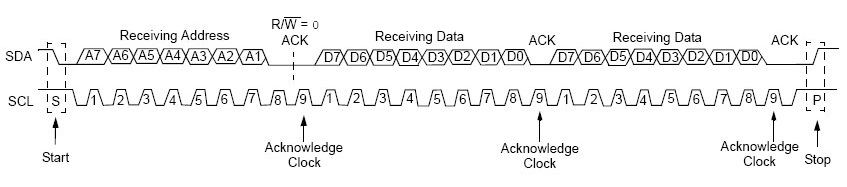
\includegraphics[width=1\linewidth]{\DocRoot/images/I2C_write}
	\caption{Typical I\textsuperscript{2}C write transmission (7-Bit Address)}
	
	\label{fig: I2C_write}
\end{figure}

When communicating with a device one will have to send a 8 bit packet. After the 8 bit a 9 bit is sent to acknowledge that the device has established a connection for communication. Note one can easily they if the master is reading from or writing to a device. If the 8 bit address is odd the master reading only and if the 8 bit address is even the writhing only.

\tocless\subsubsection{Writing to a Slave Device}
\begin{enumerate*}
	\item Send a start Sequence
	\item Send the I\textsuperscript{2}C address of the slave with R/W both low (even address)
	\item Send the internal register number one wants to write to.
	\item Send the data byte.
	\item{\bf Optional, send any further data bytes. }
	\item Send the stop sequence.
\end{enumerate*}

\newpage 

\tocless\subsubsection{Reading from Slave Device}
\begin{enumerate*}
	\item Send a start Sequence
	\item Send 0x53 ( I\textsuperscript{2}C address of the ADXL345 (accelerometer) with the R/W bit low (even address)
	\item Send 0x00  (Internal address used for device ID check )
	\item Send a start sequence again (repeated start)
	\item Send 0x53  ( I\textsuperscript{2}C address of the ADXL345  with the R/W bit high (odd address)
	\item Read data byte from ADXL345
	\item Send the stop sequence.
\end{enumerate*}

The 9DOF used in this project\footnote{\url{https://www.sparkfun.com/products/10724}} uses an accelerometer by Analog Devices  a digital Magnetometer by Honeywell and a  gyroscope  by InvenSense.

\tocless\subsection{ADXL345 Accelerometer}
The I\textsuperscript{2}C address for this devices is Ox53 (followed by the R/$\bar{\mathrm{W}}$ bit). This translates to OxA6 for the write and OxA7 for a read (See page 10 of data sheet\footnote{\url{https://www.sparkfun.com/datasheets/Sensors/Accelerometer/ADXL345.pdf}}) 

\tocless\subsection{HMC5883L Magnetometer}
The I\textsuperscript{2}C address for this devices is Ox1E. This translates to Ox3C for write and Ox3D for a read (See page 17 of data sheet\footnote{\url{https://dlnmh9ip6v2uc.cloudfront.net/datasheets/Sensors/Magneto/HMC5883L-FDS.pdf}} ) 


\tocless\subsection {ITG-3200 Gyroscope}
The I\textsuperscript{2}C address of this device is Ox68 as the $\mathrm{A}_0$ is tied to ground. This translates to OxD0 for the write and OxD1 for a read (See page 18 of data sheet\footnote{\url{https://www.sparkfun.com/datasheets/Sensors/Gyro/PS-ITG-3200-00-01.4.pdf}} )
\chapter{Week 3: 6\textsuperscript{th}  - 12\textsuperscript{th} Oct}
 \tocless\section{Objectives}
\begin{itemize}
	\item Begin Modelling
	\item Begin I\textsuperscript{2}C communication with the 9DOF
\end{itemize}

%\section{Autonomous Navigation for Flying Robots}
%All ESCs can be connected to the same I$^2$C bus.

 \tocless\section{Modelling}
To create an accurate model for the control of the quad-rotor physical measurements of the quad-rotor had to be carried out. The that have to be measured are as follows the motor gain and time constants $(K_f  ~\mathrm{and} \tau)$ , the inertia of the three axes ($J_{\theta},J_{\phi}~ \mathrm{J_{\psi}}$). 

To ensure that the model is complete enough for a first pass model one would also need to measure the damping coefficient $\beta$ and the motor drag coefficient $D$. The damping coefficient can be found while doing the moment of inertia tests while the drag can be found from doing step response on the motor and back solving to find $D$ by using the general motor equation.  \footnote{Link to explanation of how brushless DC motor work\url{http://educypedia.karadimov.info/library/ems_ch12_nt.pdf}} \footnote{Link to a control assignment of a brushless DC motor (similar to the assignment done in third year) \url{http://support.ctc-control.com/customer/elearning/younkin/driveMotorEquations.pdf}}
\begin{equation}
	J\ddot{\Theta} = K_f i - \beta \dot{\Theta} - D
	\label{motor eqation}
\end{equation}
If one sets $i$ to zero in \eqref{motor eqation} one can find the drag coefficient ($D$) if the damping factor ($\beta$) is known.
Also the mass of the quad-rotor must be found, this can easily found using a spring balance or strain gauge.

 \tocless\subsection{Motor and ESC Speed Test}
The main focus for this week was to collect data that would allow the creation of a accurate model of the quad-rotor. This meant  that trust and speed data would have to be collected so characteristic curves could created. But during the initial test of all four motors  there was huge a huge difference between motor 4 and the rest of the motor characteristic responses. This meant that all four motor would have to be recalibrated to ensure that each motor would have the same characteristic responses (within margins of error).

The results of the input control signal (\gls{pwm}) vs speed can be seen in figure \ref{fig: PWM Wavelength vs Speed for Axi Motor} (Note the \gls{pwm} used in this project has a period of  20 \si[mode=text]{\milli \second} with a 1-2 \si[mode = text]{\milli \second} pulse duration. Therefore the Duty cycle of the \gls{pwm} signal is 5 - 10 \% ). The graphs that were generated were linear as expected and were plotted in Matlab with a trend line to find the slope of the best fit line for the data sets that were taken for each motor (using ployfit command). This best fix line allows the DC motors to be normalized so that one motor model can be used for the simulation. Note that in order to get a stable aggressive control the motors will have to be reverted back to there accurate model before the code is written in C++ to ensure the best possible control of the quad-rotor.


\begin{figure}[h]
	\centering
	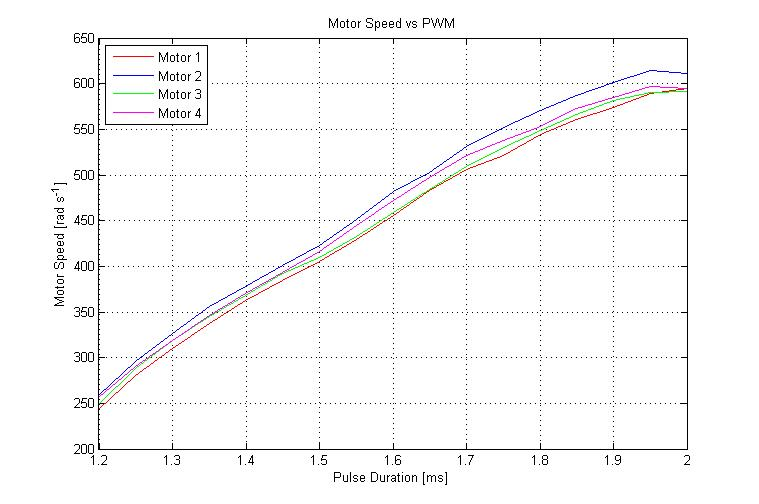
\includegraphics[width=.8\linewidth]{\DocRoot/images/SpeedPWM1}
	\caption{\gls{pwm} pulse duration vs Motor Speed}
	\label{fig: PWM Wavelength vs Speed for Axi Motor}
\end{figure}


 \tocless\subsection{Quad-Copter weight}
The mass of the quad-rotor was acquired using a strain gauge. The mass of the system was found to be 2.26 \si[mode = text]{\kilogram}. Thus the motors will have to supply 22.17  \si[mode = text]{\newton} of thrust to keep the quad-rotor to hovering in the same position. This means that each motor will have to supply at least 5.5425 \si[mode = text]{ \newton} (0.565 \si[mode =text]{\kilogram}) of thrust to keep the quad-rotor a hovering in free space.

 \tocless\subsection{Motor and Propeller Thrust}
The thrust tests were carried out using the strain gauge. The strain gauge gave out mass in \si[mode = text]{\kilogram}'s so the output had to be scaled by gravity (9.81 \si[mode = text]{\meter \per  \square \second}).  The operating point for the quad-rotor was found to be 1.7 \si[mode =text]{\milli \second} as seen in figure \ref{Fig: Motor thrust graph}.  Note this was different to the operating point found by Brendan Barry. Note fro figure \ref{Fig: Motor thrust graph} there is a head room of 10 \si[mode = text ]{\newton}. This means the maximum angle the quad-rotor can go through is 45\textsuperscript{o} so as to allow the quad-rotor some degree of manoeuvrability in 3d space. But if the limit the angle to 20\textsuperscript{o}, the quad-rotor will be capable of lifting 0.8 \si[mode = text]{\kilogram}. 
\begin{figure}[h]
	\centering
	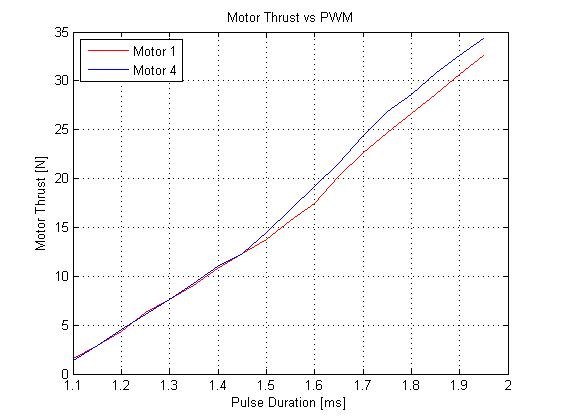
\includegraphics[width=.8\linewidth]{\DocRoot/images/ThrustPWM1}
	\caption{PWM pulse duration vs Motor Thrust}
	\label{Fig: Motor thrust graph}
\end{figure}

 \tocless\section{Communication with 9DOF}
Basic communication with the 9 DOF was accomplished using the i2c\_in (used to write to the device) and  i2c\_out (used to read from the device) during the week. There was problems communicating with the accelerometer as register 2D was entering sleep mode randomly after a revision to the code was made. The register would go from 0x08 (measurement mode) to 0x00 (wakeup mode) and the x-axis, y-axis and z-axis would then read back 0,0,0 respectfully. This problem has be insulated and hopefully code for reading the 9DOF will be in the following week.
%Time constant of motor must be found. Use a small DC motor attached to shaft of Axi motor. Apply step input. Measure DC value from motor. Use 63 percent value to find tau.

%Thrust vs PWM wave relationship must be found. Use newton balance to find relationship. Use similar set up to one shown in A2 of Brendan Barry report. Set scales to zero. Apply PWM wave get weight in kg and convert to Newton Thrust. L %inearize the data in Matlab.

%Motor speed vs PWM wave relationship must also be found. Optical Tachometer used to measure speed of rotation in rpm. Convert rpm to rad/s. Add a second order trend line to find operating point. Linearize at operating point.
%Done

%Inertia tests must be carried out for the frame. The roll and pitch axis can be presumed to be the same. Yaw is different. Ensure batteries, electronics  and sensors are mounted on the test rig. Otherwise inertia values won't be %correct. Add a substitute mass to the centre for microcontroller and associated electronics. Measure magnitude and frequency of oscillation with a voltage across a pot. Calibrate the pot for maximum angles using spirit level. Measure %using Arduino the voltage across. And convert to degrees. Using equations on page 25 of Brendan Barry report calculate various quantities.


%Drag and Inertia of the motors and drag torque of propellers need to be calculated. Find the no load torque in Figure 5.10 on page 26. Add weights to lever at end of shaft until internal resistance overcome. 

%Motor constant of Axi motor given in datasheet. Can be tested for to confirm. 

%Use current transformer to measure currents at different operating speeds.

%Find the operating point. Find weight of quad. Operating point is here for hover. So divide by 4 to spread thrust required evenly over 4 motors.

%Use this to find operating point of PWM wave in secs and speed in rad/s and current in amps.

%Where does the force to angular acceleration constant come from in Simulink diagram

%Magnetic Declination is -17$^{\circ}$ 22' West
%\chapter{Week 4: 13\textsuperscript{th}  - 19\textsuperscript{th} Oct}
 \tocless\section{Objectives}
\begin{itemize}
	\item Finish I\textsuperscript2C communication with accelerometer and magnetometer
	\item Understand how to acquire angles from the 9DOF output data (even if one is not hovering)
\end{itemize}

 \tocless\section{Accelerometer}
\subsection{Theory behind Accelerometer}
The accelerometer is used to measure the direction of the gravity vector, g\textsuperscript I , in order to define the pitch and roll angles; let it be taken as constant, pointing down along $U_D$ with an intensity $g_0$ = 9.81 $\mathrm{m~s^{-2}}$ and let
$\bar{\bf a}^B$ denote the accelerometer measurement vector.

The accelerometer used in the project ADXL345 uses the piezoelectric effect to create electric signal due to accelerative forces due to the structure used in the measure accelerometer (micro-crystal structure). Knowing how the device works one can write the following equation.

\begin{equation}
\bar{\bf a}^B = \gls{rotationmatrix}g^I - a^B +\mu_a+ \gls{accbais}  \label{eq:acc full equation}
\end{equation}
Where: $\bar{\bf a}^B$is the sensor output in $\mathrm{m~s^{-2}}$;  g\textsuperscript I is the gravity vector in the inertial frame; a\textsuperscript B is the acceleration of the craft; $\mu_a$ is the Gaussian noise component; $\mathrm{b}_a$ is the constant bias of the accelerometer.


Note if the 9DOF stick is placed at the centre of mass or close to it \eqref{eq:acc full equation} can  be shown to simplify to \eqref{eq:acc simplified equation}. Note  \eqref{eq:acc simplified equation} doesn't account for the fact that quad-rotor could be in free
fall in a horizontal position. If this occurred the output of the accelerometer should be 0. This could be a problem if one is not aware of it.

\begin{equation}
		\begin{bmatrix}
		\gls{ax}\\ \gls{ay} \\\gls{az} 
		\end{bmatrix}
		= 
		g
		\begin{bmatrix}
		-S_{\gls{pitch}}\\ C_{\gls{pitch}}S_{\gls{roll}}\\C_{\gls{pitch}}C_{\gls{roll}} 
		\end{bmatrix}
		+
		\begin{bmatrix}
		\mu_{m-x}\\ \mu_{m-y}\\\mu_{m-z}
		\end{bmatrix}		
		+
		\begin{bmatrix}
		\gls{accbaisx}\\ \gls{accbaisy}\\\gls{accbaisz}
		\end{bmatrix}
\label{eq:acc simplified equation}
\end{equation}

 \tocless\subsection{Accelerometer code}

\begin{algorithm}
	\caption{Communication with Accelerometer}\label{Alg: acclermeter setup}
	\begin{algorithmic}[1]
	\Procedure{Accelerometer setup}{}
	\State {Device\_ID} \gets {Register{\bf 0x00} value} 									\Comment {Should return 0xE5}
	
	        \If{Device\_ID$ \neq \mathrm{0xE5}$}
	        \Return Error with Accelerometer
	        \EndIf
	        
	\State  {Register {\bf 0x2C }} \gets {\bf 0x0B}  											\Comment {Set sampling rate to 200 Hz}
	\State  {Register {\bf 0x2D }} \gets {\bf 0x08}												\Comment{Set device to measure mode}
	\State {Register {\bf 0x38 }} \gets {\bf 0x84}														\Comment{Set FIFO to stream}
	\EndProcedure
	\end{algorithmic}
\end{algorithm}

	\begin{algorithm}
		\caption{Read data from Accelerometer}\label{Alg: read from accel}
		\begin{algorithmic}[1]
		\Procedure{Read data from Magnetometer}{}
		\While{Accelerometer availble}		
		\State{Reg\_Read[]} \gets { Registers $0\mathrm{x}32 ~ \mathrm{to}~ 0\mathrm{x}38 $}. 		\Comment {Read devices registers}
		\For {$i := 0 ~ \mathrm{to}~ 6 ~\mathrm{step} ~2$ }
		\State {Results[$i$/2] } \gets {\bf Convert\_2\_sgn}(Reg\_Read[$i$+1],Reg\_Read[$i$])
		\EndFor	
		%		\State Concatenate (0x33 and 0x32), (0x35 and 0x34) and  (0x37 and 0x36) which are the X,Y and Z registers respectably.
		%		\State {\bf Results} = XOR the concatenated results with 0x00FF, add 1 and multiply by -1 (convert from 2's complement). 
		\State \Return {Results}
		\EndWhile
		\EndProcedure
	\end{algorithmic}
\end{algorithm}


 \tocless\subsection{Theory behind Compass}
The compass is a sensor designed to detect the magnetic North direction, written as {\bf  N\textsuperscript I}. By the definition of the reference frame and neglecting  magnetic inclination and magnetic declination, {\bf  N\textsuperscript I} = [1,0,0]\textsuperscript T.

A Honeywell HMC5883L was used in this project. The device works by measuring the change in resistance with a change in the applied magnetic field. The device can measure these change as it is made from strips of permalloy. As the device can measure the change in magnetic field, the orientation of the magnetic field can be estimated. Let $\bar{N}^B$ be the sensor measurement; considering the frame system, a Gaussain measurement noise, $\mu_m$, and a bias term, $b_m$. Knowing these values the following equation can be defined.
\begin{equation}
	\bar{\bf N}^B = \gls{rotationmatrix}N^I + \mu_m + \gls{gyrobais} \nonumber
\end{equation}

\begin{equation}
		\begin{bmatrix}
		\bar{\bf N}_x \\ \bar{\bf  N}_y \\\bar{\bf  N}_z 
		\end{bmatrix}
		= 
		\begin{bmatrix}
		C_{\gls{pitch}}C_{\gls{yaw}}\\ C_{\gls{yaw}}S_{\gls{roll}}S_{\gls{pitch}} - C_{\gls{roll}}S_{\gls{yaw}}\\C_{\gls{yaw}}C_{\gls{roll}}S_{\gls{pitch}} + S_{\gls{roll}}S_{\gls{yaw}}
		\end{bmatrix}
		+
		\begin{bmatrix}
		\mu_{m-x}\\ \mu_{m-y}\\\mu_{m-z}
		\end{bmatrix}		
		+
		\begin{bmatrix}
		\gls{gyrobaisx}\\ \gls{gyrobaisy}\\\gls{gyrobaisz}
		\end{bmatrix}\label{eq: magnetometer read out}			
\end{equation}



When the quad-rotor is hovering, one can assume that the compass is held horizontally ($\gls{pitch} = \gls{roll} = 0$) and \eqref{eq: magnetometer read out} simplifies to \eqref{eq: mag read out simp}.


\begin{equation}
\begin{bmatrix}
\bar{\bf  N}_x \\ \bar{\bf  N}_y \\\bar{\bf  N}_z 
\end{bmatrix}
= 
\begin{bmatrix}
C_{\gls{yaw}}\\ - S_{\gls{yaw}}\\0
\end{bmatrix}
+
\mu_{m}
+
b_{m}
\label{eq: mag read out simp}
\end{equation}

 \tocless\subsection{Compass code}

\begin{algorithm}
	\caption{Communication with Magnetometer}\label{Alg: Magnetometer setup}
	\begin{algorithmic}[1]
		\Procedure{Magnetometer setup}{}
	\State {Device\_ID} \gets {Register{\bf 0x0A} value} 									\Comment {Should return 0x48}
	
	\If{Device\_ID$ \neq \mathrm{0x48}$}
	\Return Error in Magnetometer
	\EndIf
	
	\State  {Register {\bf 0x00 }} \gets {\bf 0x78}  											\Comment {Set number of samples to average}
	\State  {Register {\bf 0x01}} \gets {\bf 0xA0}												\Comment{Set gain {LSB/Gauss} }
	\State {Register {\bf 0x02 }} \gets {\bf 0x00}														\Comment{Set mode to continues-measurement mode}
	\EndProcedure
	\end{algorithmic}
\end{algorithm}

\begin{algorithm}
	\caption{Read data from Magnetometer}\label{Alg: read from Magnetometer}
	\begin{algorithmic}[1]
		\Procedure{Read data from Magnetometer}{}
		\While{Accelerometer availble}		
		\State{Reg\_Read[]} \gets{ Registers $0\mathrm{x}32 ~ \mathrm{to}~ 0\mathrm{x}38 $}.
		\For {$i := 0 ~ \mathrm{to}~ 6 ~\mathrm{step} ~2$ }
		\State {Results[$i$/2] } \gets { Gain\_Factor*\bf Convert\_2\_sgn}(Reg\_Read[$i$],Reg\_Read[$i$+1]) %\comment{Note registers are aranged in X,Z,Y}
		\EndFor
%		\State Concatenate (0x33 and 0x32), (0x35 and 0x34) and  (0x37 and 0x36) which are the X,Y and Z registers respectably.
%		\State {\bf Results} = XOR the concatenated results with 0x00FF, add 1 and multiply by -1 (convert from 2's complement). 
		\State \Return {Results}
		\EndWhile
		\EndProcedure
	\end{algorithmic}
\end{algorithm}


\begin{algorithm}
	\caption{Convert 2s complement to decimal}\label{Alg:  2's complement to decimal}
	\begin{algorithmic}[1]
	\Function{Convert\_2\_sgn}{MSB,LSB}	
	
	Con\_Array \gets ((Reg\_MSB <<8) \& 0xFF00) | (Reg\_LSB \& 0xFF)
	
	\If {Con\_Array >= 0x8000}		
	\State Con\_array \gets Con\_array $\oplus$  0xFFFF 
	\State Con\_array \gets Con\_array +1
	\State Con\_array \gets  -1 * Con\_array
	\EndIf
	\Return  Con\_array
	\EndFunction
	\end{algorithmic}
\end{algorithm}

The \ref{Alg: auto tune of comp filter} worked well and gave a adequate  filtering when using the values returned by the program.

\chapter{Week 5: 20\textsuperscript{th}  - 26\textsuperscript{th} Oct}


 \tocless\section{Objectives}
\begin{itemize}
	\item Find the moments of inertia of the about all three axes.
\end{itemize}

 \tocless\section{Inertia about each axis}
To find the moment of inertia of the quad-rotor the rig was held by cable  at it's end point and allowed to swing about a single axis. To document the amplitude of the quad-rotor at each oscillation a laser pointer was attached to the end of the quad-rotor \footnote{This was done so one could acquire the damping of the system about each axis after the test was completed}and to record the period of each oscillation a stop watch \footnote{This was done so one could a quire the moment of inertia about each axis}. The oscillation was carried out about a low friction surface to ensure an accurate value for the moment of inertia of each axis. The results were entered into Matlab and the following results were acquired for the moment of inertia of the system.


\begin{align}
I =  
\begin{bmatrix}
\gls{interiaofroll}  & 0 & 0 \\ 0& \gls{interiaofpitch} & 0 \\0& 0& \gls{interiaofyaw}
\end{bmatrix}
=
\begin{bmatrix}
0.1274 & 0 & 0 \\ 0& 0.1221& 0 \\0& 0& 0.2370
\end{bmatrix}
\label{eq: moment of interia of the system}
\end{align} 



Note as the system is symmetric about the pitch and roll axis one can assume that $\gls{interiaofroll}   =\approx \gls{interiaofpitch}$.

 \tocless\section{Damping}

 The results for the maximum amplitude were processed using Matlab and the results were plotted yielding figure \ref{fig: plot of angle vs time}.
\begin{figure}[t]
	\centering
	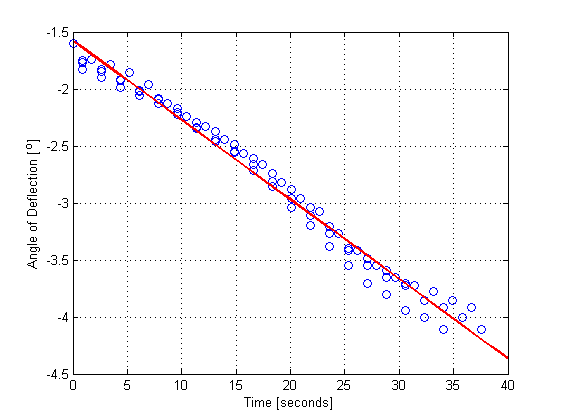
\includegraphics[scale = 1]{\DocRoot/images/moment_inertia}
	\caption{Plot of deflection from normal  vs Time}
	\label{fig: plot of angle vs time}
\end{figure}

From figure \ref{fig: plot of angle vs time} one can acquire the moment of inertia from the slope of the line and thus define the inertia of the system as follows. 

\begin{align}
\beta =  
\begin{bmatrix}
\gls{dampingroll}  & 0 & 0 \\ 0& \gls{dampingpitch} & 0 \\0& 0& \gls{dampingyaw}
\end{bmatrix}
=
\begin{bmatrix}
 0.0194 & 0 & 0 \\ 0&  0.0194 & 0 \\0& 0&  \approx 0
\end{bmatrix}
\label{eq: damping of the system}
\end{align} 

\chapter{Week 6: 27\textsuperscript{th} Oct  - 2\textsuperscript{nd} Nov }

 \tocless\section{Objectives}



\begin{itemize*}
	\item Create the state space equations for the roll and pitch.
	\item Make the Simulink model for the Kalman Filter.
\end{itemize*}

 \tocless\section{Derivation of state space equations for Kalman filter}
The following kalman equation was taken from the \cite{Artofcontrol} and can be seen on page 483 and the derivation of the equation can be seen on page 791 of the same book
\begin{equation}
\hat{\bf x}_{k+1|k+1} = \Phi\hat{\bf x}_{k|k} + {\bf \varDelta u}_{k} + {\bf K}[{\bf z}_{k+1} - {\bf C}(\Phi \hat{\bf x}_{k|k} + {\bf\varDelta u }_k) ] \label{eq : kalman gain from art of control long}
\end{equation}

\ref{eq: kalman equation from art of control } is the same \ref{eq : kalman gain from art of control long} but the matrix/variables are grouped together for ease of computation.
\begin{equation}
	\hat{\bf x}_{k+1|k+1} = [{\bf I -KC}][\Phi \hat{\bf x}_{k|k} +\varDelta{\bf u}_k] + {\bf Kz}_{k+1} \label{eq: kalman equation from art of control }
\end{equation}

\ref{eq: kalman equation from art of control } can be written as follows.
\begin{equation}
	\hat{\bf x}_{k+1|k+1} = { F}\hat{\bf x}_{k|k} + { H}{\bf u}_k + {\bf Kz}_{k+1} \label{Eq: Kalman Equation Representation used in our report}
\end{equation}
Where in \ref{Eq: Kalman Equation Representation used in our report} ${ F} =  [{\bf I -KC}]\Phi$; $H =  [{\bf I -KC}]\varDelta $. Thus each matrix is made up of a mix of prediction and current value with the exception of the Kalman gain $\bf K$.

 
\begin{equation}
	\begin{bmatrix}																
		\hat{x}_1		         			\\
		\hat{ x}_2		
		\end{bmatrix}_{k+1}
		=
	\begin{bmatrix}
		F_{11}	& F_{12 } \\
		F_{21}	& F_{22}
		\end{bmatrix}
			\begin{bmatrix}											
			\hat{\bf x}_1		         			\\
			\hat{\bf x}_2		
			\end{bmatrix}_{k}	
			+
	\begin{bmatrix}
	H_1 \\
	H_2
	\end{bmatrix}
	{\bf u}_k
	+
	\begin{bmatrix}
	K_{11}	& K_{12 } \\
	K_{21}	& K_{22}
	\end{bmatrix}
	\begin{bmatrix}											
	{ z}_1		         			\\
	{z}_2		
	\end{bmatrix}_{k+1}	
\end{equation}

{\bf Where:} ${\bf x_1}$ is angular velocity ${\bf \alpha}$ and ${\bf x_2}$ is angular acceleration $\dot{\bf \alpha}$  

\newpage
 \tocless\section{Simulink model of Kalman filter}
\begin{figure}[h]
	\centering
	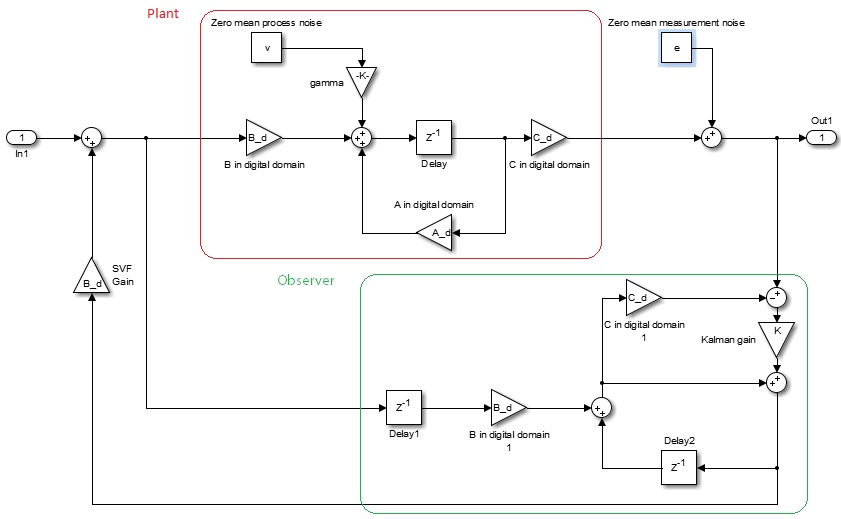
\includegraphics[scale = 0.5]{\DocRoot/images/Full_kalman_model2}
	\caption{Full Kalman Filter Model with plant as seen in \cite{Artofcontrol} pg 483}
	\label{fig: Kalman model}
\end{figure}

The Simulink model in figure \ref{fig: kalman used in project} is the observer model used in this project and how it interacts with the plant can be seen in \ref{fig: Kalman model}. Note in this project the Kalman gain {\bf K} is set and is not adjusted during flight.

\begin{figure}[h]
	\centering
	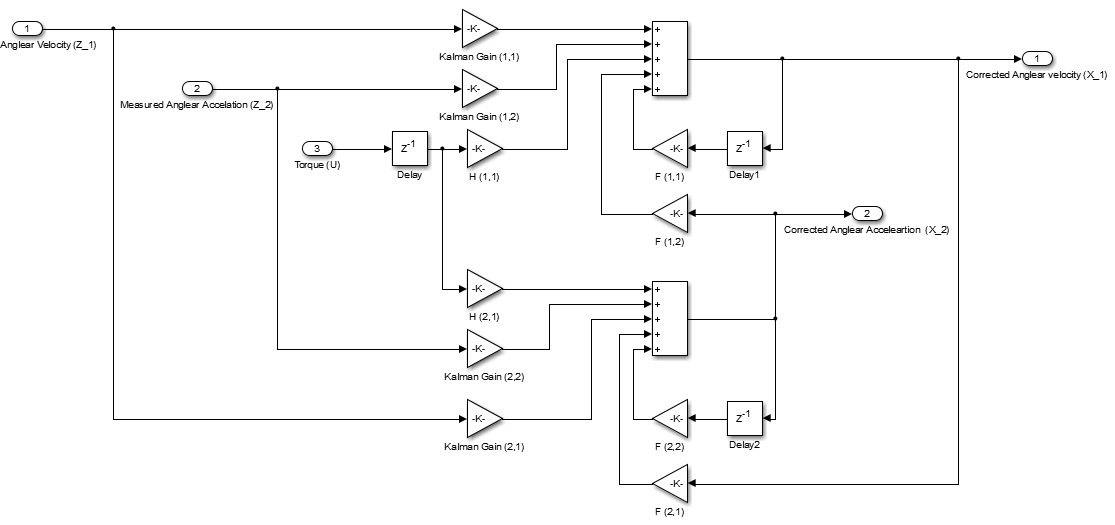
\includegraphics[scale = 0.4]{\DocRoot/images/Kalman_gordon_model}
	\caption{Simplified model of the Kalman filter}
	\label {fig: kalman used in project}
\end{figure}

\chapter{Week 7: 3\textsuperscript{rd} - 9\textsuperscript{th} Nov }

\tocless\section{Objectives}



\begin{itemize*}
	\item Read up on methods to remove bias from sensors.
	\item Analysis and remove offset/mean from accelerometer and gyroscope.
	\item Come up with a method to find the {\bf R} matrix of the system.
\end{itemize*}


\tocless\section{Accelerometer Bias }
Due to the fact of the large bias on the accelerometer a method had to be found in order to reduce it, a better model made to be found or the Kalman filter had to be remodelled. The method agreed approved to deal with this problem and hopefully the correct one is the methods discussed in the following papers
\cite{acclerometer_bais,Accelrometer_bias}. Upon using the sensors there were sensor bias error, however, the sensors can read something different that the required (ideal) at a given location due to many factors including mechanical tolerances in the component parts.


The way to measure and remove bias error from the accelerometer is to do the following:- 

\begin{enumerate}
	\item Place the sensor module on an approximately horizontal surface (table top, granite flat, etc.).
	\item Rotate the sensor module $90^o$ to each of the positions shown in
	      Figure
	\item Read the outputs on each axis in each of the six positions.
	\item Calculate the sensitivities (where the first subscript is the sensor, the second subscript is the position):
	      \begin{equation}
		      S_{xx} = \frac{(a_{x2} - a_{x4})}{2};~~S_{yy} = \frac{(a_{y1} - a_{y3})}{2};~~S_{zz} = \frac{(a_{z5} - a_{z6})}{2};
	      \end{equation}
	      
	\item
	      Calculate the sensor module biases:
	      
	      \begin{multline}
		      B_x^{0g} = \left(\frac{a_{x1}+a_{x3}+a_{x5}+a_{x6}}{4}\right);~~ B_y^{0g} = \left(\frac{a_{x2}+a_{x4}+a_{x5}+a_{x6}}{4}\right);\\B_z^{0g} = \left(\frac{a_{x1}+a_{x2}+a_{x3}+a_{x4}}{4}\right);
	      \end{multline}
	      
	\item Save $B_x^{0g}, ~ B_y^{0g},~B_z^{0g},~S_{xx},~S_{yy},~\mathrm{and}~S_{zz}$ local and use these values in all subsequent calculations of the acceleration to get the correct outputs.
\end{enumerate}

\begin{figure}[h]
	\centering
	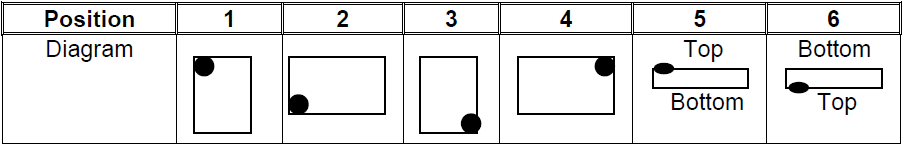
\includegraphics[width =0.6 \paperwidth]{\DocRoot/images/Bias}
	\caption{Position in which one has to measure the bias for calibration}
	\label{Fig: Position to measure the bias}
\end{figure}

\tocless\section{Formula to measure angle}
\tocless\subsection{Measuring Tilt Angle using One Axis}
Accelerometers measure acceleration. That is acceleration due to movement and also acceleration due to gravity. If you want to measure tilt in both $x$ and $y$ axis with a 2-axis accelerometer then you can simply use $\sin x$ where $x$ is the output from one axis of the accelerometer. Remember that beyond +45 and -45 degrees the accuracy will diminish

\tocless\subsection{Measuring Tilt Angle using Three Axis}
For accurate measurements of tilt in both the $x ~\mathrm{\&}~ y $ planes the following formulas have to be used\footnote{See \url{http://www.hobbytronics.co.uk/accelerometer-info} for more details}
.

\begin{align}
	\begin{split}
		\gls{pitch} &= \arctan\left(\frac{\gls{ax}}{\sqrt{\gls{ay}^2 + \gls{az}^2}}\right)\\
		\gls{roll} &= \arctan\left(\frac{\gls{ay}}{\sqrt{\gls{ax}^2 + \gls{az}^2}}\right)
	\end{split}
\end{align}

%\chapter{Week 8: 10\textsuperscript{th} Oct  - 16\textsuperscript{th} Nov }

\section{Objectives}



\begin{itemize*}
	\item Collect data to allow the acquirement of {\bf R}.
	\item Find the matrix {\bf R}.
\end{itemize*}


\titleformat{\chapter}
{\normalfont\LARGE\bfseries}
{}{0.0em}{}




\chapter{Week 1: 19\textsuperscript{th} - 25\textsuperscript{th} January }

 \tocless\subsection{Accelerometer model}
In order to implement the complementary filter a model of the accelerometer had to be created that links the data output of the device to the actual angle of the quad-rotor, hence the following equations where developed.

\begin{equation}
\begin{bmatrix}
\gls{ax} \\ \gls{ay} \\\gls{az}
\end{bmatrix}
= 
g
\begin{bmatrix}
-S_{\gls{pitch}}\\ C_{\gls{pitch}}S_{\gls{roll}}\\C_{\gls{pitch}}C_{\gls{roll}} 
\end{bmatrix}
+
\begin{bmatrix}
\mu_{m-x}\\ \mu_{m-y}\\\mu_{m-z}
\end{bmatrix}		
+
\begin{bmatrix}
\gls{accbaisx}\\ \gls{accbaisy}\\\gls{accbaisz}
\end{bmatrix}
\label{eq:acc simplified equation}
\end{equation}

Now if one assumes that the bias and noise on the accelerometer is zero (can be removed in code)  one can find the angle of the Quad-rotor in the \gls{ned} frame . Hence the \gls{roll} and \gls{pitch} can be defined as follows:-

\begin{align}
\begin{split}
\gls{roll} &= \arctan\left(\frac{\gls{ay}}{\gls{az}}\right)\\
\gls{pitch} &= \arctan \left(\frac{- \gls{ax}}{\sqrt{\gls{ay}^2+\gls{az}^2}}\right)
\label{Eq: angles from acc}
\end{split}
\end{align} 

 \tocless\subsection{Gyroscope model}
A similar model for the gyroscope was created as the angular velocity measured by the gyroscope does not correspond to the Euler angle rates $[\dot{\gls{roll}},\dot{\gls{pitch}},\dot{\gls{yaw}}]^\intercal$ . Instead one can define the rate of change of angle with respect to the earth frame \gls{ned} as follows:-


\begin{equation}
\begin{bmatrix}																
\gls{wx}         			\\
\gls{wy} 	  \\
\gls{wz}
\end{bmatrix} =
\begin{bmatrix}																
1	& 0						 & -S_{\gls{pitch}}           			\\
0 	& C_{\gls{roll}}   & S_{\gls{roll}}C_{\gls{pitch}}   \\
0 	& -S_{\gls{roll}}  & C_{\gls{roll}}C_{\gls{pitch}}\end{bmatrix}
\begin{bmatrix}																
\dot{\gls{roll} }        			\\
\dot{\gls{pitch}} 	  \\
\dot{\gls{yaw}}\end{bmatrix}
\end{equation}

Now taking the in the inverse one gets the following:-
\begin{equation}
\begin{bmatrix}																
\dot{\gls{roll} }        			\\
\dot{\gls{pitch}} 	  \\
\dot{\gls{yaw}}
\end{bmatrix}
=
\begin{bmatrix}																
1	& S_{\gls{roll}}T_{\gls{pitch}}	 & C_{\gls{roll}}T_{\gls{pitch}}           			\\
0 	& C_{\gls{roll}}   & -S_{\gls{roll}}  \\
0 	& \frac{S_{\gls{roll}} }{C_{\gls{pitch}}} & \frac{C_{\gls{roll}}}{C_{\gls{pitch}}}
\end{bmatrix}
\begin{bmatrix}																
\gls{wx}         			\\
\gls{wy} 	  \\
\gls{wz}
\end{bmatrix} 
\label{Eq: angleur velocity from gyro}
\end{equation}

 \tocless\section{ Complementary Filter}
A pair of filters are called complementary filters if their transfer functions sum to one at all frequencies in a complex sense, i.e. the phase is zero and the magnitude is one \ref{eq: bases of comp filter}.


\begin{equation}
G_1(s) + G_2(s) =1 \label{eq: bases of comp filter}
\end{equation}

 \tocless\subsection{First Order Complementary Filter}

To start with a first order complementary filter was design using \eqref{eq: filter order filter}. This first order filter had adequate results.
\begin{equation}
\gls{filterdata} = \underbrace{\frac{1}{1 + \tau s}}_{\text{$G_1(s)$}}\gls{accdata} + \underbrace{\frac{\tau s}{1 + \tau s}}_{\text{$G_2(s)$}}\frac{1}{s}\gls{gyrodata}
\label{eq: filter order filter}
\end{equation}


Using \eqref{Eq: angles from acc}, \eqref{Eq: angleur velocity from gyro} and\eqref{eq: filter order filter} the high frequency components of the estimated orientation angles where found by a high-pass filter on the gyroscope data:-
\begin{align}
	\dot{\gls{roll}}_{hp} &=   \gls{wx} + S_{\gls{roll}}T_{\gls{pitch}}\gls{wy} + C_{\gls{roll}}T_{\gls{pitch}}\gls{wz}   - \frac{\gls{roll}_{hp}}{\tau}\\
	\dot{\gls{pitch}}_{hp} &=  C_{\gls{roll}}\gls{wy} - S_{\gls{roll}}\gls{wz} - \frac{\gls{pitch}_{hp}}{\tau}
\end{align}

Similarly the low-pass equivalents are found using the following:-

\begin{align}
\dot{\gls{roll}}_{lp} &=   \frac{1}{\tau}\left[\arctan\left(\frac{\gls{ay}}{\gls{ay}}\right) - \gls{roll}_{lp}\right]\\
\dot{\gls{pitch}}_{lp} &=  \frac{1}{\tau}\left[\arctan\left(\frac{-\gls{ax}}{\sqrt{\gls{ay}^2+\gls{az}^2}}\right) - \gls{pitch}_{lp}\right]
\end{align}

 \tocless\subsection{Difference Equations for first order filter}
\eqref{eq: filter order filter} was emulated into the digital domain using Tustain's approximation to integration. Tustain's method was chosen as it ensures a stable mapping into the discrete domain (maps to inside the unit circle) if the continues function is stable, forward rectangular rule and backward rectangular rule do not ensure this. \footnote{See \url{http://web.cecs.pdx.edu/~tymerski/ece452/6.pdf} for more details}.

\begin{equation}
\gls{filterdata} [k] = \frac{1}{\gls{ts} + 2\tau}(\gls{ts} ( \gls{accdata} [k] + \gls{accdata} [k-1] + \tau(\gls{gyrodata} [k]+\gls{gyrodata} [k-1])) -(\gls{ts} -2\tau)\gls{filterdata} [k-1] )
\end{equation}

Note it can be easily shown that if there is a bias \gls{accbaisx} on the $x$-axis of the gyroscope then there will be an offset angle when one integrates the gyroscope reading. For the first order filter this offset (for the $x$-axis)can be approximated by use of the filter time constant and is defined as follows:-

\[\theta_{offs} \approx {\tau}\gls{accbaisx} \]
 \tocless\subsection{Second Order Complementary Filter}

A complementary filter is easily derived by solving the transfer function of the Mahony \& Madgwick filter for the angle $\theta$, which yields

\begin{equation}
\gls{filterdata}=\underbrace{ {\frac{K_i + K_p s}{K_i + K_p s + s^2}}}_{\text{$G_1(s)$}}\gls{accdata} + \underbrace{\frac{s^2}{K_i+K_p s + s^2}}_{\text{$G_2(s)$}}\frac{1}{s}\gls{gyrodata}
\label{eq: second order filter}
\end{equation}

Obviously, and not unexpectedly, this complementary filter is build from $2^{\mathrm{nd}}$ order filters. Note that the filter acting on the acceleration data actually consists of a low-pass plus band-pass filter.

This result has interesting consequences. Being $2^{\mathrm{nd}}$ order filters, the frequency response of the acceleration and rotation rate filters are characterized by the resonance frequency and damping factor

\begin{equation}
\omega_0 = \sqrt{K_i}~~~~~~~ \xi = \frac{K_p}{2\sqrt{K_i}}
\end{equation}

The damping factor determines the overshoot at the resonance frequency. For high-pass (and low-pass) filters the frequency response is flat (and the step response non-oscillatory) for $\xi \geq 1$. This suggests the criterion \footnote{See \url{http://www.olliw.eu/2013/imu-data-fusing/} for more details}.

\begin{equation}
K_i \leq \frac{1}{4}K_p^2
\end{equation}


To find the a method of modelling the filter in MatLab $G_1(s)$ and $G_2(s)$ where arranged as follows:-
\begin{align}
\chi_{hp} &= \frac{1}{s}\left[\gls{gyrodata} - \chi_{hp}\left({\frac{K_i}{s} + K_p}\right)\right] \label{Eq: second order comp high pass second}\\
\chi_{lp}  &= \frac{1}{s}\left[(\gls{accdata} - \chi_{lp})\left({\frac{K_i}{s} + K_p}\right)\right] \label{Eq: second order comp low pass second}
\end{align}


Note \eqref{Eq: second order comp high pass second} and \eqref{Eq: second order comp low pass second} can be combined to yield the following filter (as $\chi_{hp} + \chi_{lp} =  \gls{filterdata} $), which can also be modelled in MatLab.

\begin{equation}
\gls{filterdata}  = \frac{1}{s}\left[\gls{gyrodata} +\left({\frac{K_i}{s} + K_p}\right)(\gls{filterdata}   - \gls{accdata})\right] \label{eq: comp filter equation used to tune comp filter}
\end{equation}


 \tocless\subsection{Difference Equations for second order filter}
\eqref{Eq: second order comp high pass second}, \eqref{Eq: second order comp low pass second} were emulated into the digital domain using Tustain's method, which yielded the following equations:-
\begin{align}
\chi_{hp}[k] &= \frac{1}{\eta + 4}\left(2\gls{ts} ( \gls{gyrodata} [k] - \gls{gyrodata} [k -2] ) - (\Gamma + 4)\chi_{hp}[k-2] - (\xi - 8)\chi_{hp}[k-1] \right) \label{Eq: second order comp high pass second difference eq}\\
\chi_{lp}[k]  &= \frac{1}{\eta +4}\left(\Gamma \gls{accdata} [k-2] + \xi \gls{accdata} [k-1] + \eta \gls{accdata} [k] - (\Gamma + 4)\chi_{lp}[k-2] - (\xi - 8) \chi_{lp}[k - 1] \right) \label{Eq: second order comp low pass second difference eq}
\end{align}


where:-

\begin{equation*}
\eta = K_i\gls{ts}^2 + 2K_p\gls{ts};~~~ \Gamma = K_i\gls{ts}^2 - 2 K_p\gls{ts};~~~ \xi = 2K_i\gls{ts}^2
\end{equation*}

Note \eqref{Eq: second order comp high pass second difference eq} and \eqref{Eq: second order comp low pass second difference eq} can be combined to give the following:-

\begin{multline}
\gls{filterdata} [k] = \frac{1}{\eta +4}(\Gamma \gls{accdata} [k-2] + \xi \gls{accdata} [k-1] + \eta \gls{accdata} [k] + 2\gls{ts} ( \gls{gyrodata} [k] \\
- \gls{gyrodata} [k -2] )   - (\Gamma + 4)\gls{filterdata} [k-2] - (\xi - 8) \gls{filterdata} [k - 1] ) \label{Eq: full dfference equation for the second order filter}
\end{multline}




\chapter{Week 2: 26\textsuperscript{th} January - 1\textsuperscript{st} February }
 \tocless\section{Objectives}


\begin{itemize*}
	\item Acquire an accurate Drag Coefficient (\gls{dragcoofmotor}) so as the Yaw axis could be controlled correctly.
	\item Help with the design of the Integral Action on the Roll and Pitch axes.
	\item See if one can use system identification (least squares) to tune the complementary filter.
	\item Design an algorithm to self tune the Complementary Filter.
\end{itemize*}


 \tocless\section{Drag coefficient Test}
Upon reviewing the drag coefficient from previous years it was suspected that it was incorrect as it was a hundred times less than the drag coefficients (\gls{dragcoofmotor}) found in similar quad-rotor project reports (see any of the reports in the current research section in the introduction).  To measure the force produced by the quad-rotor a strain gauge was attached to an end point of the quad-rotor and the distance from the point of rotation to the point of attachment was recorded. Two motor where then turned on and the force in the \gls{yaw}-direction was measure by means of the strain gauge. Note the measurement on the strain  is in $kg$ so it was scaled by 9.81 m s$^{-2}$ to get force, this was taken to be correct as the stain gauge pre-calibrates by using gravity to related the force applied to it to mass acting on it. The motor speed \gls{rotationalvelocity} was also measured using an optical tachometer.This was
repeated for several \gls{pwm} inputs to the motors. These experimental values were then
used to calculate drag. Using the following one can relate the drag coefficient (\gls{dragcoofmotor})  to force and \gls{rotationalvelocity} :-

\begin{align}
\begin{split}
\gls{reactiontorquedrag} &= \gls{dragcoofmotor}\gls{rotationalvelocity}^2 \\
\tau &= r \times F \\
\gls{reactiontorquedrag} &=\frac{r \times F}{\gls{rotationalvelocity}^2}
	\end{split}
	\end{align}

 \tocless\section{Design of Integral Action using DLQR}
The group felt that Integral Action was needed on the \gls{pitch} \& \gls{roll} axes, thus  Integral Action was required as a pre-compensator is not as robust in the face of modelling errors as in Integral Action. Note these modelling errors poses problems when one is designing controllers using the \gls{lqr} method as the performance will not be as \enquote{Optimal} as the design predicts, but that is a discuss that is far to long to be featured here \footnote{For more details please see Chapter 12 of \cite{Artofcontrol}, a great introduction to optimal control, and for more information please read up on \textit{\gls{dmre}}. See \cite{Discrete_control_systems} Section 7.3 and \cite{Digital_control_system_analysis_and_design} Section 10.6 for more detail on \gls{dmre}}. There are many ways to achieve integral control, in this report it was decided to add extra states to the system model which are the time integrals of the real states. If the extra state is called $z$ (not to be confused with the sensor measurement \gls{measurement}) then.
\begin{equation} 
z = \int x ~~\mathrm{dt}~~~\mathrm{or}~~~\dot{z} = x \label{eq: intregral action}
\end{equation}
 
 In the discrete time \eqref{eq: intregral action} can be written as follows:-
 
 \begin{equation}
 z_{k+1} = z_n  + \gls{ts}x_n 
 \end{equation}
 
 With the addition of this state the system can now be written as follows:-
 
 \begin{equation}
 \left[\begin{array}{c} x \\ z\end{array}\right]_{k+1} =  \left[\begin{array}{cc} \gls{Transitionmatrix} & 0\\ \gls{Cmatrix}\gls{ts} & I\end{array}\right]  \left[\begin{array}{c} x\\ z\end{array}\right]_{k} +  \left[\begin{array}{c} \gls{Bmatrix}\\ 0 \end{array}\right] u_k \label{eq: system with intergral action}
 \end{equation}
 
 Hence \eqref{eq: system with intergral action} can be written as follows, where the tildes represent the augmented vector and matrices:
 \begin{equation}
 \tilde{x}_{k+1} = \tilde{\gls{Transitionmatrix}}\tilde{x}_n + \tilde{\gls{Bmatrix}}u_k
 \end{equation}
 
 Hence using the \gls{dlqr}optimal control approach, one will get a matrix of optimal gains that satisfy the following control law:- 
 
 \begin{equation}
 u_n = - \left[\begin{array}{cc}
 K_k^p &K_k^I 
 \end{array}\right]\left[\begin{array}{c} x\\ z\end{array}\right]_{k} 
 \end{equation}
 
 Note as the above problem is a discrete time problem one has to use the following \gls{dlqr} cost function:-
 
 \begin{equation}
 J_k  = \frac{1}{2} \sum_{n=0}^{k-1}(x_n^\intercal Q x_n + u_n^\intercal Ru_n) + \frac{1}{2}x_n^\intercal Q_n x_n
 \end{equation}
 
  \tocless\section{Tuning of the Complementary Filter using Least Squares }
 A least squares method of tuning the filter was investigated this week. Using \eqref{eq: comp filter equation used to tune comp filter} one can tune the filter in the continues domain and then emulate it across. This can be done by making the following assumption:-
 \begin{equation}
 \gls{filterdata} = \gls{potangle}
 \end{equation} 
 
 where \gls{potangle} is the angle of the system as given by the potentiometer. Note in order to do this one also needs access to the rate of change of potentiometer angle as denoted as $\dot{\gls{potangle}}$. Hence one can develop a method of tuning the filter as follows:-
 
 
 
 \begin{align}
 \begin{split}
 \gls{potangle} &= \frac{1}{s}\left[ \gls{gyrodata} -\left(K_p + \frac{K_i}{s}\right) (\gls{potangle} - \gls{accdata})\right]\\
 s\gls{potangle} &= \left[ \gls{gyrodata} -\left(K_p + \frac{K_i}{s}\right) (\gls{potangle} - \gls{accdata})\right]\\
 \dot{\gls{potangle} }&= \left[ \gls{gyrodata} -\left(K_p + \frac{K_i}{s}\right) (\gls{potangle} - \gls{accdata})\right]\\
 \dot{\gls{potangle} } - \gls{gyrodata}& = -\left(K_p + \frac{K_i}{s}\right) (\gls{potangle} - \gls{accdata})\\
 \underbrace{\dot{\gls{potangle} } - \gls{gyrodata}}_{\text{$B_f$}}& = \underbrace{\left[(\gls{gyrodata} - \gls{potangle} ) + \frac{(\gls{gyrodata} - \gls{potangle} )}{s} \right] }_{\text{$A_f$}} \left[\begin{array}{c} K_p\\ K_i\end{array}\right] \label{eq: placer for leasr square eqaution}
 \end{split}
 \end{align}
 
Hence using the equation developed in \eqref{eq: placer for leasr square eqaution} one can tune a continues time complementary filter of this form using the following:- 
\begin{equation}
\left[\begin{array}{c} K_p\\ K_i\end{array}\right] = (A_f^\intercal A_f)^{-1}A_f^\intercal B_f \label{eq: tuning of complmentry filter in continues time least squares}
\end{equation} 

 Note the method of tuning the filter as shown in \eqref{eq: tuning of complmentry filter in continues time least squares} was not used in this project as the grouped didn't know $\dot{\gls{potangle} }$, instead an algorithm was create to tune it which is notes in the following section
  \tocless\section{Algorithm used to self tune the Complementary Filter}
 
 Due to the fact that the group had access to the\enquote{actual} angle \gls{potangle} of the device as potentiometer. It was decided to do a search using a \gls{rmse} \eqref{eq:rmse} with a cross-correlation used to find the delay between the signals so it can be removed when checking the \gls{rmse} term.
 
 \begin{equation}
 \gls{rmse} = \sqrt{\frac{\sum_{k = 1}^{n} (\gls{filterdata} -\gls{potangle})^2}{n}} \label{eq:rmse}
 \end{equation}
 
 The cross-correlation function is defined in \eqref{eq: cross-correlation} and is commonly used in signal processing to find the measure of time-lag between to signals, hence it's use here.
 
 \begin{equation}
 (f \star g)[n] = \sum_{m = -\infty}^{\infty} f^*[m]g[m+n] \label{eq: cross-correlation}
 \end{equation}

 
 
 \begin{algorithm}
 	\caption{Auto Tuning a Complementary Filter }\label{Alg: auto tune of comp filter}
 	\begin{algorithmic}[1]
 		\Procedure{Grid search tuning of a Complementary Filter }{}
 			\State$K_{p(max)} = 50$;
 			\State$K_{i(max)} = 50$;
 			\State Grid size = 1000;
 		    \State  Previous Error = 100000000;
 		    \State $K_{p(it)}$ =linspace(0.1,$K_{p(max)}$,Grid size );
  		    \State $K_{i(it)}$ =linspace(0.1,$K_{i(max)}$,Grid size );	
  		    
  		    	    
 		\For {i := 1: (length($K_{p(it)}$)-1)}
 		
 			\For {j := 1: (length($K_{i(it)}$)-1)}
 			 		\State\gls{filterdata} = Filter output using \eqref{Eq: full dfference equation for the second order filter}
 					\State signal delay = Output of equation \eqref{eq: cross-correlation} using \gls{filterdata} and \gls{potangle} as inputs.
 					\State   \gls{filterdata} = \gls{filterdata}(signal delay :end)
 					\State    Error = Output of equation \eqref{eq:rmse} using \gls{filterdata} and \gls{potangle} as inputs.
 								\If {(Error  < Previous Error)}
 									       \State $K_p$ = $K_{p(it)}$(i);
 									        \State $K_i$ = $K_{i(it)}$ (j);
 									        \State Previous Error = Error;
 								\EndIf
 			\EndFor
 		\EndFor
 		\State \Return {$K_p$ \& $K_i$}
 		\EndProcedure
 	\end{algorithmic}
 \end{algorithm}
\chapter{Week 3: 2\textsuperscript{nd} - 8\textsuperscript{th} February }
\begin{itemize*}
	\item Find and remove bias on the sensors.
	\item Find the \gls{noisecomatrix} matrix used by the Kalman filter.
	\item Tune the Kalman Filter and compare it to the Complementary Filter. 
\end{itemize*}
	
	 \tocless\section{Sensor Bias}
	The bias on the sensors were found for the accelerometer by the means shown in figure \ref{Fig: Position to measure the bias} and they were found to be as follows:-
		\begin{equation}
		\begin{bmatrix}
		\gls{accbaisx}\\ \gls{accbaisy}\\\gls{accbaisz}
		\end{bmatrix} 
		=
		\begin{bmatrix}
		-2.223\\ 5.3447  \\9.17645
		\end{bmatrix}
		\end{equation}
		
		The bias on the gyroscope was found by placing the sensor on a flat surface and left to settle for five minutes so that the sensors would only measure there offsets and were found to be as follows:-
		
				\begin{equation}
				\begin{bmatrix}
				\gls{gyrobaisx}\\ \gls{gyrobaisy}\\\gls{gyrobaisz}
				\end{bmatrix} 
				=
				\begin{bmatrix}
				-34.163 \\ 20.156  \\-88.66
				\end{bmatrix}
				\end{equation}
	 \tocless\section{Measurement of the \gls{noisecomatrix} matrix}
ax It was possible to measure the \gls{noisecomatrix}  covariance matrix by obtaining various measurement from the sensors and estimating the noise present. The results were read to m-file and the covariance found using \textit{cov(x)} function in \textit{MatLab}. Hence the \gls{noisecomatrix}  matrix was calculated as follows:-
					\begin{equation}
			\gls{noisecomatrix}_a  = 		
                   \left[\begin{array}{ccc}
					\mathrm{cov(\gls{roll})}       &                 0                          & 0\\ 
					                                     0       & \mathrm{cov(\gls{pitch})}           & 0\\
					                                      0         &                0                          &\mathrm{cov(\gls{yaw})}
					\end{array} \right]
					\end{equation}
					Where \textit{cov(\gls{roll})} denotes the covariance of the \gls{roll} angle from the expected value.
	
Hence $\gls{noisecomatrix}_a$ was found as follows:-
						\begin{equation}
						\gls{noisecomatrix}_a  = 		
						1.0e-03\left[\begin{array}{ccc}
						0.2710      &                 0                          & 0\\ 
						0       & 0.1980           & 0\\
						0         &                0                          &NaN
						\end{array} \right]
						\end{equation}

By a similar manner one can find the $\gls{noisecomatrix}_g$ and define it as follows:-
	
							\begin{equation}
							\gls{noisecomatrix}_g  = 		
							1.0e-05\left[\begin{array}{ccc}
							0.1264      &                 0                          & 0\\ 
							0       & 0.2221           & 0\\
							0         &                0                          &0.0757
							\end{array} \right]
							\end{equation}
	
			 \tocless\section{Tuning of the Kalman Filter}
			Calculating the \gls{noisecoplantmatrix} matrix proved to be a much more difficult task. Very little real information regarding the noise present in the states was known. However, one method of tuning the filter is to leave on of the matrix fixed and scale the other as it is the ratio of \gls{noisecoplantmatrix} / \gls{noisecomatrix} which is important as seen in \cite{gordon_paper}. Hence, it was found that the ratio of the parameters affected the response and to a less degree the individual parameter values. Therefore \gls{noisecomatrix} was set to the theoretical value calculated and \gls{noisecoplantmatrix}  varied until an optimal response was achieved. The results of tuning the filter can be seen in figure {Fig: Kalman Filter Estimate and Complementary Filter Estimate }
	
		
\begin{figure}[h]
	\centering
	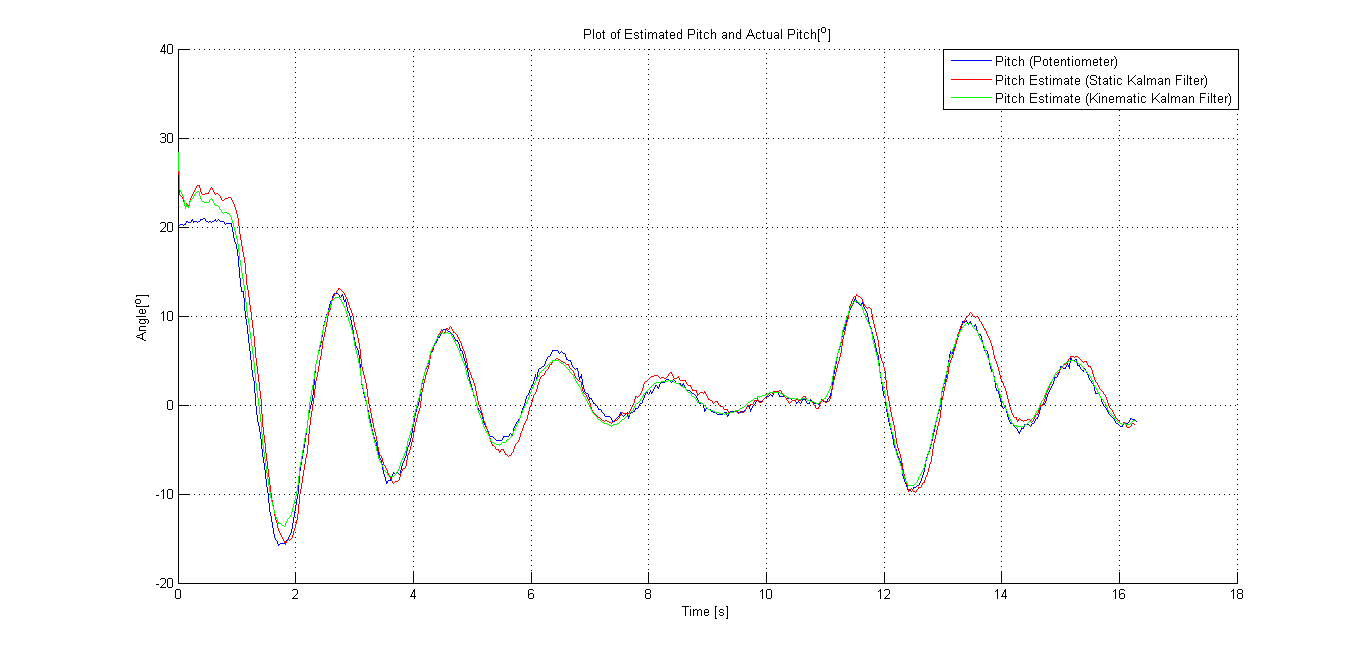
\includegraphics[width =0.6 \paperwidth, height = 7cm]{\DocRoot/images/kalman_comp}
	\caption{Plot of Kalman Filter Estimate, Complementary Filter Estimate and Actual Angle of the device}
	\label{Fig: Kalman Filter Estimate and Complementary Filter Estimate }
\end{figure}

For the above graph $K_{p\gls{pitch}}$ and $K_{i\gls{pitch}}$ are equal to 3.5902 and 2.0522 respectively. While \gls{kalmangain} was found to be as follows:-

							\begin{equation}
							\gls{kalmangain}_{\gls{pitch}}  = 		
							\left[\begin{array}{cc}
							0.032064         &      0.0001017                         \\ 
							0.0085871       &     0.996498           
							\end{array} \right]
							\end{equation}


	 \tocless\section{Chart Depicting how the Kalman Filter Works}
		\begin{center}
			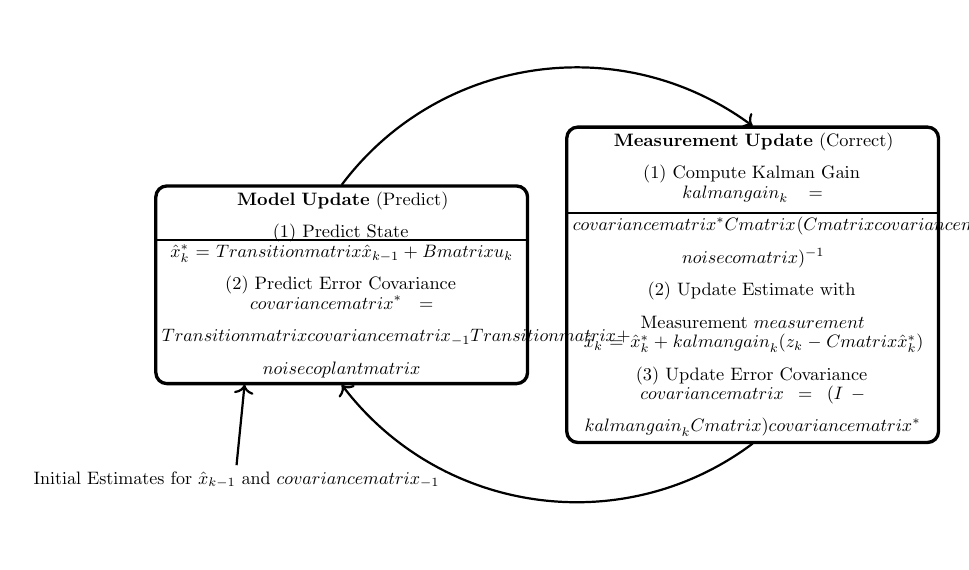
\begin{tikzpicture}[scale=0.65, transform shape]
			
			%
			% Styles for states, and state edges
			%
			\tikzstyle{state} = [{rectangle, rounded corners, draw=black, very thick, text width=20.0em, minimum height=4em, text centered}]
			\tikzstyle{stateEdgePortion} = [black,thick];
			\tikzstyle{stateEdge} = [stateEdgePortion,->];
			\tikzstyle{edgeLabel} = [pos=0.5, text centered, font={\sffamily\small}];
			
			
			%
			% Position States
			%
			\node[state, name=predict] {{{\LARGE}{\bf Model Update} (\enquote{Predict})}   \\ 
				{   (1) Predict State  \\  \vspace{-0.25cm}
					\hh $\hat{x}^{*}_{k} = \gls{Transitionmatrix}\hat{x}_{k-1} + \gls{Bmatrix}u_{k}$\\ 
					(2) Predict Error Covariance \\ \vspace{-0.25cm}
					\hh $\gls{covariancematrix}^* = \gls{Transitionmatrix}\gls{covariancematrix}_{-1}\gls{Transitionmatrix}^{\intercal} + \gls{noisecoplantmatrix}$}};
			
			
			\node[state, name=correct, right of=predict, xshift=20em] {{\bf Measurement Update} (\enquote{Correct}) \\ 
				{   (1) Compute Kalman Gain\\  \vspace{-0.25cm}
					\hh $\gls{kalmangain}_{k} = \gls{covariancematrix}^*\gls{Cmatrix}^{\intercal}(\gls{Cmatrix}\gls{covariancematrix}^*\gls{Cmatrix}^{\intercal} + \gls{noisecomatrix})^{-1}$\\ 
					(2) Update Estimate with Measurement $\gls{measurement}$ \\ \vspace{-0.25cm}
					\hh $\hat{x}_k = \hat{x}^{*}_k + \gls{kalmangain}_k(z_k - \gls{Cmatrix}\hat{x}_k^{*})$\\
					(3) Update Error Covariance  \\ \vspace{-0.25cm}
					\hh $\gls{covariancematrix} = (I - \gls{kalmangain}_k\gls{Cmatrix})\gls{covariancematrix}^{*}$
					
				}};
				
				
				%
				% Connect States via edges
				%
				\draw (predict.north) 
				edge[stateEdge, bend left=45] node[edgeLabel, xshift=-3em]{} 
				(correct.north); 
				
				\draw ($(predict.west) + (0,2.5em)$) 
				edge[stateEdgePortion] node[edgeLabel, yshift=+2.1cm]{} 
				($(predict.east) + (0,2.5em)$); 
				
				\draw (correct.south) 
				edge[stateEdge, bend left=45] node[edgeLabel, xshift=-3em]{} 
				(predict.south); 
				
				\draw ($(correct.west) + (0,4.0em)$) 
				edge[stateEdgePortion] node[edgeLabel, yshift=+2.1cm]{} 
				($(correct.east) + (0,4.0em)$); 
				
				
				
				% 
				% inital states to start the filter
				%
				\node[ name=inital, below of=predict, left of=predict, xshift = -3em ,yshift=-8em]{Initial Estimates for $\hat{x}_{k-1}$ and $\gls{covariancematrix}_{-1}$};
				
				\draw ($(inital.north) + (0,0)$) 
				edge[stateEdge] node[edgeLabel, yshift=+2.1cm]{} 
				($(predict.south) + (-5.4em,0)$); 
				\end{tikzpicture}
			\end{center}

\chapter{Week 4: 9\textsuperscript{th} - 15\textsuperscript{th} February }

\begin{itemize*}
	\item Tune the Kalman Filter that uses a pure kinematic system model (i.e is independent of a control input matrix)
	\item Read up on non-linear control
	\item  Investigate the \gls{ekf} as it is commonly used in GPS systems 
\end{itemize*}

 \tocless\section{Tuning of a Kalman Filter that uses a pure kinematic}
This it was decided  to look at and tune an adaptive kalman filter which  does no depend on the controller  plant inputs. This filter was modelled as follows and is commonly used on quad-rotors.

 \begin{equation}
 \dot{\gls{rotationmatrix}}=  \underbrace{\left[\begin{array}{ccc} 0 & \gls{wz} & -\gls{wy}\\ -\gls{wz} & 0 & \gls{wx}\\ \gls{wy}&-\gls{wx} & 0 \end{array}\right] }_{\text{\gls{skewmatrix}}} \gls{rotationmatrix} \label{eq: rate of chage of roatation matix}
 \end{equation} 

As the gravity is fixed in the \gls{ned} frame, it must be converted to the \gls{bf} frame as the accelerometer and gyroscope are fixed to the quad-rotor. Since gravity acts in the $z$-direction, the third column of the rotation matrix \gls{rotationmatrix} can be used to approximate \gls{roll} and \gls{pitch} of the quad-rotor and hence \eqref{eq: rate of chage of roatation matix}can be redefined as follows knowing that gravity is taken to act in the $z$-direction.

\begin{equation}
\dot{\gls{rotationmatrix}}_3=  \gls{skewmatrix} \gls{rotationmatrix}_{3}\label{eq: adtive kalman eqautions}
\end{equation}

The continuous state space equation of \eqref{eq:state space adative kalman equations} therefore represents the system under control.

\begin{align}
\begin{split}
\dot{\underline{x}} &= \gls{skewmatrix}\underline{x}\\
\underline{y}              &= \underline{x}
\end{split}
\label{eq:state space adative kalman equations}
\end{align}

However, \eqref{eq:state space adative kalman equations} is a continuous state space equation. This must be converted to the discrete version since the Kalman Filter must be implemented in discrete form, which is achieved as follows:-
 
 \begin{align}
\begin{split}
 \underline{x}_k &= \gls{Transitionmatrix}x_{k-1}\\
 \underline{y}_k              &= \underline{x}_k
\end{split}
 \end{align}

This filter was tuned in a similar manner to the Kalman filter seen last week and the two filters are compared in figure \ref{Fig: Kalman Filter Estimate and Kinematic Kalman Filter Estimate}. Note the two filters give almost identical results (the one featured this week is slightly better), but the filter featured this week is more computational intensive (as \gls{Transitionmatrix} varies with time)and does not allow one to filter the gyroscope outputs. I light of these drawbacks the filters works well and would be better suited to systems who's model are hard to develop.
						\begin{figure}[h]
							\centering
							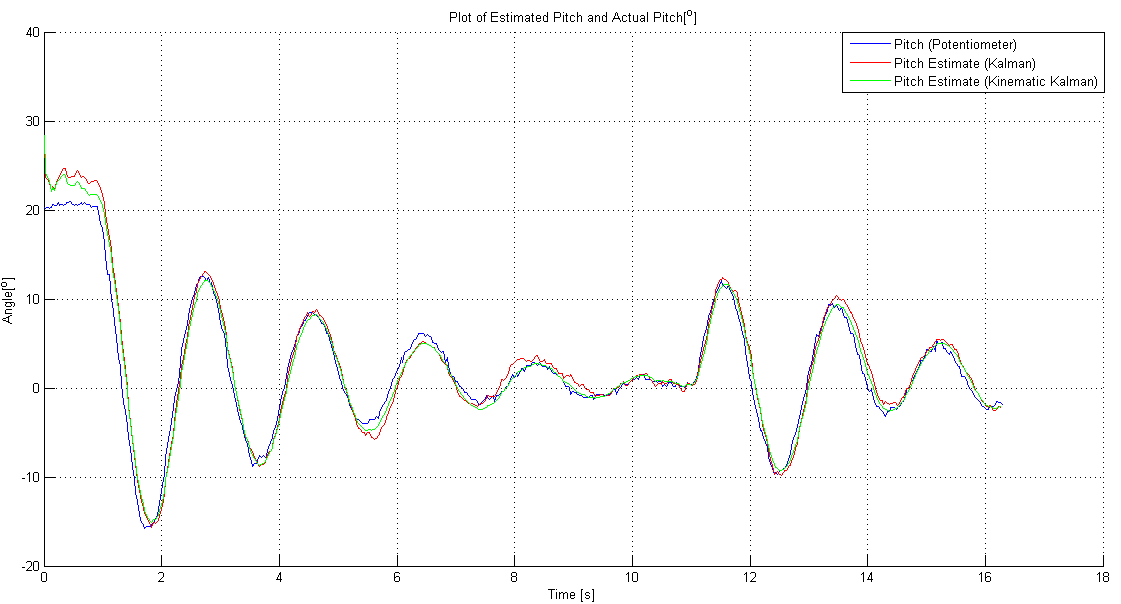
\includegraphics[width =0.7\paperwidth, height = 10cm]{\DocRoot/images/kalman_filter_comparsion}
							\caption{Plot of Kalman Filter Estimate, Kinematic Kalman Filter Estimate and Actual Angle of the device}
							\label{Fig: Kalman Filter Estimate and Kinematic Kalman Filter Estimate}
						\end{figure}




 \tocless\section{Introduction to the \gls{ekf} and associated code}
As the measurement function $h(x_k,\gls{noiseinoutput}_k)$ of the gyroscope is a non-linear function it was decided that it might be worth while looking at a more advanced kalman filter which is capable of dealing with non-linear systems, thus the \gls{ekf} was explore. Note as the group wanted to implement a \gls{gps} system on the quad-rotor the \gls{ekf} was the natural choice as it is the de-facto filter used in \gls{gps} systems \cite{An_Introduction_to_the_Kalman_Filter}. 


In something akin to a Taylor series, one most linearise the system around the current
estimate using the partial derivatives of the process and measurement functions to
compute estimates even in the face of non-linear relationships. The process is governed by the \textit{non-linear} stochastic difference equation:-
\begin{equation}
x_k = f(x_{k-1},u_k,\gls{noiseinsysystem}_{k-1})
\end{equation}
and the measurement model by the following stochastic difference equation:-
\begin{equation}
z_k = h(x_k,\gls{noiseinoutput}_k)
\end{equation}

where the random variables \gls{noiseinsysystem} and \gls{noiseinoutput} again represent the process and measurement
noise.



In practice of course one does not know the individual values of the noise \gls{noiseinsysystem} and \gls{noiseinoutput}  at
each time step. However, one can approximate the state and measurement  without
them as follows:-

\begin{equation}
x_k^* = f(\hat{x}_{k-1},u_k,0) \label{eq: ekf approximate the state }
\end{equation}
and the measurement model by the following stochastic difference equation:-
\begin{equation}
z_k = h(x_k^*,0)  \label{eq: ekf approximate the measurement}
\end{equation}

It is important to note that a fundamental flaw of the \gls{ekf} is that the distributions of the various random variables are no longer normal
after undergoing their respective non-linear transformations. The \gls{ekf} is simply an ad-hoc
state estimator that only approximates the optimality of Bayes’ rule by linearisation.


\eqref{eq: ekf approximate the state } is linearised around the control input $u_k$ and the previous estimate using \eqref{eq: jacobain of fx} and the measurement function \eqref{eq: ekf approximate the measurement} is linearised around the $x_k^*$  using  \eqref{eq: jacobain of hx}
\begin{equation}
A_k=\left.\left[\begin{array}{cccc}
\frac{\partial f_{1}}{\partial x_1} &\frac{\partial f_{1}}{\partial x_2} &\dots& \frac{\partial f_{1}}{\partial x_n}\\
\frac{\partial f_{2}}{\partial x_1} &\frac{\partial f_{2}}{\partial x_2} &\dots& \frac{\partial f_{2}}{\partial x_n}\\
\vdots& \vdots& \ddots &\vdots\\
\frac{\partial f_{n}}{\partial x_1} &\frac{\partial f_{n}}{\partial x_2} &\dots&\frac{\partial f_{n}}{\partial x_n} \\
\end{array}\right]\right|_{\hat{x}_k,u_k} \label{eq: jacobain of fx}
\end{equation}

\begin{equation}
C_k=\left.\left[\begin{array}{cccc}
\frac{\partial h_{1}}{\partial x_1} &\frac{\partial h_{1}}{\partial x_2} &\dots& \frac{\partial h_{1}}{\partial x_n}\\
\frac{\partial h_{2}}{\partial x_1} &\frac{\partial h_{2}}{\partial x_2} &\dots& \frac{\partial h_{2}}{\partial x_n}\\
\vdots& \vdots& \ddots &\vdots\\
\frac{\partial h_{n}}{\partial x_1} &\frac{\partial h_{n}}{\partial x_2} &\dots&\frac{\partial h_{n}}{\partial x_n} \\
\end{array}\right]\right|_{\hat{x}_k^*} \label{eq: jacobain of hx}
\end{equation}

Note the above Jacobian can be calculated at each stage on a micro-controller by using the Cauchy’s integral
formula which is defined as follows\cite{Jacobain_approx_paper}:-


\begin{equation}
f^{(n)}(z) = \frac{n!}{2\pi i}\oint_\gamma \frac{f(\kappa)}{(\kappa - z)^{n+1}}d\kappa \label{eq: Cauchy's intrgral formula}
\end{equation}

If one wants to implement \eqref{eq: Cauchy's intrgral formula} on a micro-controller one has to approximated it a closed form power series as follows:-

\begin{equation}
f^{(n)}(z) \approx \frac{n!}{mh} \sum_{j=0}^{m-1}\frac{f(z+h e^{i\frac{2 \pi j}{m}})}{e^{i\frac{2 \pi j n}{m}}}
\end{equation}

The derivation of a complex-step derivative (first partial derivative) approximation is done by an approximation of a non-linear function with a complex variable using the Taylor's series expansion.

\begin{equation}
f(x+ih) = f(x) + ihf^{'} (x) - h^2\frac{f^{''}(x)}{2!}- ih^3\frac{f^{'''}(x)}{3!}+h^4\frac{f^{4}(x)}{4!} + \dots
\end{equation}

Now taking only the imaginary parts of both sides gives
\begin{equation}
\mathrm{Im}[f(x+ih)] = hf^{'}(x) - h^3\frac{f^{'''}(x)}{3!}+\dots \label{eq: imaginary parts of  Cauchys integral approx}
\end{equation}
Dividing by $h$, rearranging and assuming terms higher than $h^2$ or higher can be ignored since the interval $h$ can be chosen up to the precision of the machine (smallest difference the machine can produce) and thus \eqref{eq: imaginary parts of  Cauchys integral approx} can be approximated as follows:-
\begin{equation}
f^{'}(x) = \mathrm{Im}[f(x+ih)]/h \label{eq: how to do differenation on a controller}
\end{equation}
As \eqref{eq: how to do differenation on a controller} is not a function of differences it is more accurate than standard finite difference and more inportantly one can now calculate a  partial derivative on a micro-controller using \eqref{eq: how to do differenation on a controller} 


	 \tocless\section{Chart Depicting how the \gls{ekf} Works}
	\begin{center}
		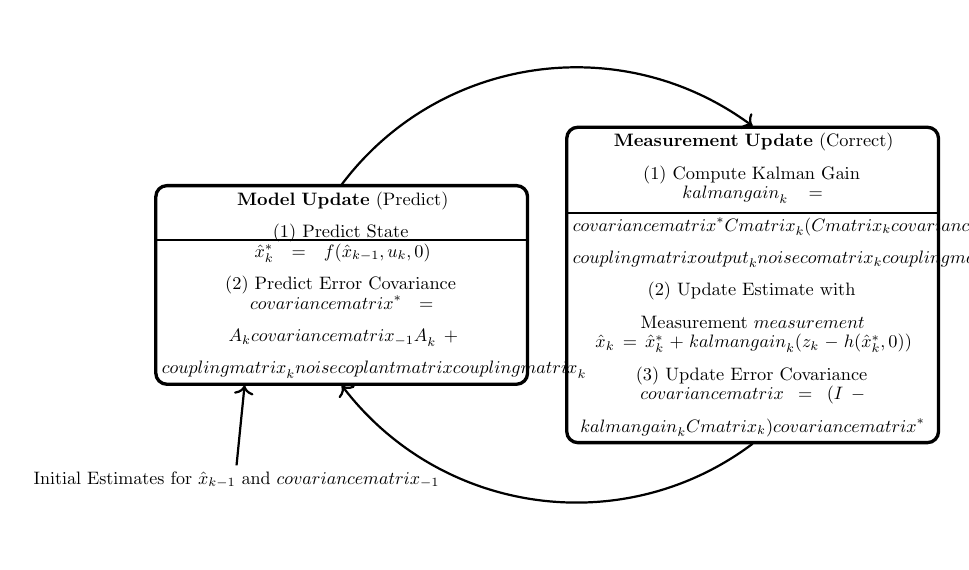
\begin{tikzpicture}[scale=0.65, transform shape]
		
		%
		% Styles for states, and state edges
		%
		\tikzstyle{state} = [{rectangle, rounded corners, draw=black, very thick, text width=20.0em, minimum height=4em, text centered}]
		\tikzstyle{stateEdgePortion} = [black,thick];
		\tikzstyle{stateEdge} = [stateEdgePortion,->];
		\tikzstyle{edgeLabel} = [pos=0.5, text centered, font={\sffamily\small}];
		
		
		%
		% Position States
		%
		\node[state, name=predict] {{{\LARGE}{\bf Model Update} (\enquote{Predict})}   \\ 
			{   (1) Predict State  \\  \vspace{-0.25cm}
				\hh $\hat{x}^{*}_{k} = f(\hat{x}_{k-1},u_k,0)$\\ 
				(2) Predict Error Covariance \\ \vspace{-0.25cm}
				\hh $\gls{covariancematrix}^* = A_k\gls{covariancematrix}_{-1}A_k^{\intercal} + \gls{couplingmatrix}_k\gls{noisecoplantmatrix}\gls{couplingmatrix}_k^{\intercal}$}};
				
				
				\node[state, name=correct, right of=predict, xshift=20em] {{\bf Measurement Update} (\enquote{Correct}) \\ 
					{   (1) Compute Kalman Gain\\  \vspace{-0.25cm}
						\hh $\gls{kalmangain}_{k} = \gls{covariancematrix}^*\gls{Cmatrix}_k^{\intercal}(\gls{Cmatrix}_k\gls{covariancematrix}^*\gls{Cmatrix}_k^{\intercal} + \gls{couplingmatrixoutput}_k\gls{noisecomatrix}_k\gls{couplingmatrixoutput}_k^{\intercal})^{-1}$\\ 
						(2) Update Estimate with Measurement $\gls{measurement}$ \\ \vspace{-0.25cm}
						\hh $\hat{x}_k = \hat{x}^{*}_k + \gls{kalmangain}_k(z_k - h(\hat{x}^{*}_{k},0))$\\
						(3) Update Error Covariance  \\ \vspace{-0.25cm}
						\hh $\gls{covariancematrix} = (I - \gls{kalmangain}_k\gls{Cmatrix}_k)\gls{covariancematrix}^{*}$
						
						}};
						
						
						%
						% Connect States via edges
						%
						\draw (predict.north) 
						edge[stateEdge, bend left=45] node[edgeLabel, xshift=-3em]{} 
						(correct.north); 
						
						\draw ($(predict.west) + (0,2.5em)$) 
						edge[stateEdgePortion] node[edgeLabel, yshift=+2.1cm]{} 
						($(predict.east) + (0,2.5em)$); 
						
						\draw (correct.south) 
						edge[stateEdge, bend left=45] node[edgeLabel, xshift=-3em]{} 
						(predict.south); 
						
						\draw ($(correct.west) + (0,4.0em)$) 
						edge[stateEdgePortion] node[edgeLabel, yshift=+2.1cm]{} 
						($(correct.east) + (0,4.0em)$); 
						
						
						
						% 
						% inital states to start the filter
						%
						\node[ name=inital, below of=predict, left of=predict, xshift = -3em ,yshift=-8em]{Initial Estimates for $\hat{x}_{k-1}$ and $\gls{covariancematrix}_{-1}$};
						
						\draw ($(inital.north) + (0,0)$) 
						edge[stateEdge] node[edgeLabel, yshift=+2.1cm]{} 
						($(predict.south) + (-5.4em,0)$); 
						\end{tikzpicture}
						\end{center}

\chapter{Week 5: 16\textsuperscript{th} - 22\textsuperscript{nd} February }

\begin{itemize*}
	\item Interface with GPS module 
	\item  Test the control and filter code on the quad-rotor
	\item Use the Kalman Filter to filter the GPS
\end{itemize*}

 \tocless\section{Testing }
Most of the week was sent testing the control and filters on the quad-rotor. It was found that the delay on the second order complementary filter was to large so the Kalman filter was implemented on the chip. The first order filter was also investigated to see if the delay could be reduced, it was and the results of the filtering can be seen in figure \ref{Fig: Kalman Filter Estimate and First Order complementary Filter}:-



						\begin{figure}[h]
							\centering
							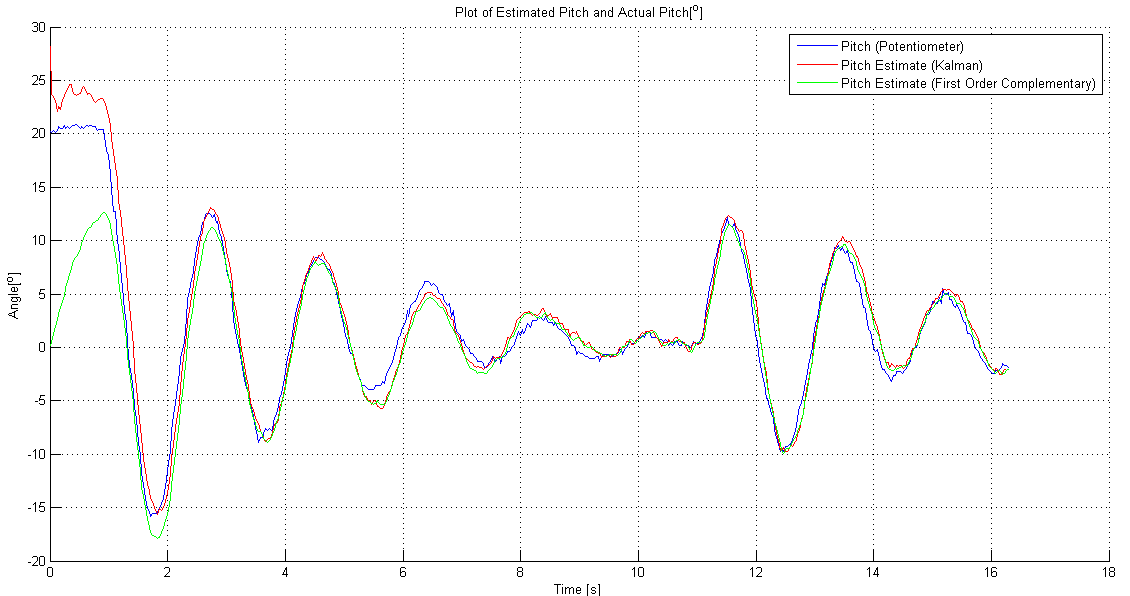
\includegraphics[width =0.7\paperwidth, height = 10cm]{\DocRoot/images/First_order_filter_vs_kalman}
							\caption{Plot of Kalman Filter Estimate, First Order complementary Filter and Actual Angle of the device}
							\label{Fig: Kalman Filter Estimate and First Order complementary Filter}
						\end{figure}
						
Note as the findings in figure \ref{Fig: Kalman Filter Estimate and First Order complementary Filter} are promising the filter overshoots when there is high accelerations, the Kalman Filter doesn't have such draw backs. The complementary filter presented in figure \ref{Fig: Kalman Filter Estimate and First Order complementary Filter} has a filter parameter of $\tau = 0.5$.						


 \tocless\section{GPS Mapping \& Associated Equations}	

If one wants to control the quad-rotor using differential equations based on $x,y,z$ coordinate system one will have to map the latitude (\gls{latitude}) and longitude (\gls{longitude}) values given by the \gls{gps} sensor.	Note that any mapping \enquote{unwrapping} of a spherical objecting onto a flat plane will cause distortions and loss of information (this was first mathematically proven by C. F. Gauss). Methods of doing this mapping will now be presented:-

 \tocless\subsection{Transverse Mercator Projection}
 The Transverse Mercator Projection or Gauss–Kr\"{u}ger projection is a conformal mapping of the earth ellipsoid where a central meridian is mapped into a straight line at constant scale. It is widely used in national and international mapping systems around the world and hits a middle ground between computational ease and accuracy. In order to preform this projection one places a model of the Earth on a cylinder as seen in figure \ref{Fig:  Transverse_Mercator_projection} and \enquote{roll} the cylinder to form a conventional map\cite{utm}.
 
 
 \begin{figure}[h]
 	\centering
 	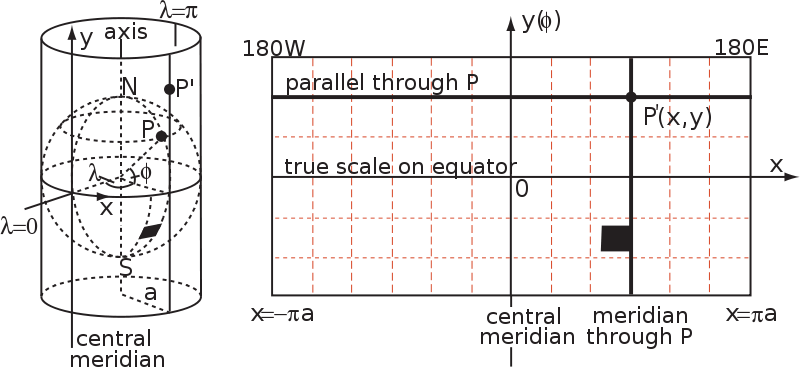
\includegraphics[width =0.7\paperwidth]{\DocRoot/images/Transverse_Mercator_projection}
 	\caption{Normal aspect of a tangent cylindrical project of a sphere (Transverse Mercator projection)}
 	\label{Fig:  Transverse_Mercator_projection}
 \end{figure}
 
 Using the project defined by figure \ref{Fig:  Transverse_Mercator_projection} one can calculate \gls{east} \& \gls{north} coordinates using the following assuming the $y$-axis goes through the  Prime Meridian in Greenwich. 
 \begin{align}
\begin{split}
 \gls{east}(\gls{longitude},\gls{latitude}) &= \frac{1}{2}k_o a \ln\left[\frac{1 + \sin\gls{longitude}\cos\gls{latitude}}{1 - \sin\gls{longitude}\cos\gls{latitude}}\right]\\
 \gls{north}(\gls{longitude},\gls{latitude}) &= k_o a \arctan\left[\sec\gls{longitude}\cos\gls{latitude}\right]
\end{split}
 \end{align}
 
 Similarity, if one can to find latitude and longitude using  only \gls{east} \& \gls{north} one can use the following equations:-
 
  \begin{align}
  \begin{split}
  \gls{longitude} &= \arctan\left[\sinh\frac{\gls{east}}{k_oa} \sec\frac{\gls{north}}{k_oa}\right]\\
  \gls{latitude}(\gls{east},\gls{north}) &= k_o a \arctan\arcsin\left[\mathrm{sech}\frac{\gls{east}}{k_oa}\sin\frac{\gls{north}}{k_oa}\right]
  \end{split}
  \end{align}
  
  where:-\\
  $k_o$; is the \enquote{point scale}  and is commonly taken as  0.9996 for reasons that will not be mentioned here but are listed in \cite{utm}\\
  $a$; is the equatorial radius of the earth and is equal to 6,378,137~$m$\\
  $b$; is the polar radius of the earth and is equal to 6,356,752.3142~$m$
  
   \tocless\subsection{Universal Transverse Mercator}
 The \gls{utm} projection uses a 2-D Cartesian based system to map the locations on the surface of the earth. Note this system differs from the traditional method of latitude (\gls{latitude}) and longitude (\gls{longitude}) as it is not a single map projection.  \gls{utm} also divides the Earth into sixty \enquote{Zones} , which are six-degree bands of longitude (\gls{longitude}) and it uses the Transverse Mercator Projection in each of these \enquote{Zones} \cite{utm}.
 
 The following formulas are truncated version of the Transverse Mercator: flattening series, these formulae where first derived by J.H.L Kr\"{u}ger in 1912. The mapping use WGS 84 which describes the Earth as an oblate spheroid. In order to map from latitude and longitude (\gls{latitude},\gls{longitude}) to \gls{utm} (\gls{east},\gls{north}) one has to introduce constants to make the notation easier, this is done first:-
 
 \begin{align}
 \begin{split}
 n                 &= \frac{f}{2-f},~~                                                                                           A=\frac{a}{1+n}\left(1 + \frac{1}{4}n^2 + \frac{1}{64}n^4 + \dddot{}\right)\\
 \alpha_1 &= \frac{1}{2}n - \frac{2}{3}n^2 + \frac{5}{16n^3} + \dddot{},       ~~\alpha_2 = \frac{13}{48}n^2 - \frac{3}{5}n^3 + \dddot{},     ~~\alpha_3   = \frac{61}{240}n^3 + \dddot{}\\
 \beta_1    &= \frac{1}{2}n - \frac{2}{3}n^2+\frac{37}{96}n^3 + \dddot{},      ~~\beta_2   = \frac{1}{48}+\frac{1}{48}n^3 + \dddot{},              ~~  \beta_3   = \frac{17}{480}n^3 + \dddot{}\\
 \delta_1  &=  2n-\frac{2}{3}n^2 - 2n^3 + \dddot{},                                                      ~~ \delta_2 = \frac{7}{3}n^2 - \frac{8}{5}n^3 + \dddot{},          ~~   \delta_3 =   \frac{56}{15}n^3  + \dddot{} 
 \end{split}
 \end{align}
 
 Where: \\
 $f$: is flatting and is given by the following:- $f = (a-b)/a$ \\
 $e$: is the eccentricity of the earth and is defined as follows:- $e= \sqrt{f(2-f) }$\\


 \tocless\subsubsection{Mapping from latitude and longitude (\gls{latitude},\gls{longitude}) to \gls{utm} (\gls{east},\gls{north})}
Before one can project (\gls{latitude},\gls{longitude}) to \gls{utm} (\gls{east},\gls{north}) one has to do an interment step\footnote{Please see the following for more details and a full derivation of these formulas \cite{utm}}.

\begin{align}
	\tau^\prime &= \sinh \left(\tanh^{-1}(\sin\gls{latitude})- \frac{2\sqrt{n}}{1+n}\tanh^{-1}\left(\frac{2\sqrt{n}}{1+n}\sin\gls{latitude}\right) \right)\\
	\xi^\prime &= \tan^{-1}(\frac{\tau^\prime}{\cos(\gls{longitude} - \lambda_o)})\\
	\eta^\prime &= \sinh^{-1}\left(\frac{\sin(\gls{longitude}-\lambda_o)}{\sqrt{\tau^{\prime 2} + \cos^2\gls{longitude}}}\right)
\end{align}
	
Now that these are defined one can map 	 (\gls{latitude},\gls{longitude}) to \gls{utm} (\gls{east},\gls{north})  using the following formulas:-	

\begin{align}
\gls{east} =& k_oA\left(	\eta^\prime  + \sum_{j=1}^{3}\alpha_j\cos(2j\xi^\prime)\sinh(2j\eta^\prime)\right)\\
\gls{north} =& k_oA\left(	\xi^\prime  + \sum_{j=1}^{3}\alpha_j\sin(2j\xi^\prime)\cosh(2j\eta^\prime)\right)
\end{align}

   \tocless\subsection{Basic Method of Mapping  (\gls{latitude},\gls{longitude}) to (\gls{east},\gls{north})}
  For small angles ($1^o$) one can use the following equations:-
  
  \begin{equation}
  \Delta_{\gls{latitude}} = \frac{\pi a (1 - e^2)}{180(1-e^2\sin^2\gls{latitude})^{\frac{3}{2}}} \label{eq: delta latitude}
  \end{equation}
 
 The distance in meters (correct to 0.01 metres) between ($\gls{latitude} \pm 0.5^o$) on the \gls{wgs} 84 spheroid is given by the following formula:-
 
 \begin{equation}
  \Delta_{\gls{latitude}} =  111132.954 - 559.822\cos(2\gls{latitude}) + 1.175\cos(4\gls{latitude})
 \end{equation}
 
 Similarly  for longitude:-
   \begin{equation}
   \Delta_{\gls{longitude}} = \frac{\pi a \cos(\gls{latitude})}{180\sqrt{1-e^2\sin^2\gls{latitude}}} \label{eq: delta longtitude}
   \end{equation}

\chapter{Week 6: 23\textsuperscript{rd} February- 1\textsuperscript{st} March }
 \tocless\section{Objectives}
\begin{itemize*}
	\item Chose Mapping for GPS to find \ensuremath{xyz}
	\item Test control on the Quad-rotor
	\item  Prepare for the seminars 

\end{itemize*}


 \tocless\section{Test Quad-rotor}
Fixing issues with program run-time on Propeller took longer than planned so no progress was made on actual testing.

 \tocless\section{\gls{gps} conversion from \gls{ecef} frame to \gls{ned} frame }
In other for the Quad-rotor to be stabilized in position another frame was introduced, but before the distance to move in the \gls{ned} frame can be found the distance to travel in the \gls{ecef} has to be found. This difference can be found if one knows the latitude \gls{latitude} and longitude \gls{longitude} on is at and the latitude \gls{latitude} and longitude \gls{longitude} the Quad-rotor has to go too. Once this is know, \eqref{Eq: xyz distance in circle coordinance} can be used to find $xyz$ displacement in the \gls{ecef} and then map this displacement using \eqref{Eq: ecef frame mapping}.


\begin{align}
\begin{split}
N &= \frac{a}{\sqrt{1 - e^2\sin^2\gls{latitude}}}\\
x&= (N+h)\cos(\gls{latitude})\cos(\gls{longitude})\\
y &= (N+h)\cos(\gls{latitude})\sin(\gls{longitude})\\
z &= [N(1-e^2)+h]\sin(\gls{latitude})
\end{split}
\label{Eq: xyz distance in circle coordinance}
\end{align}

{\bf Where:-}

$h$: is the height of the quad-rotor from the surface of the planet.

\newpage
 
 
 In order to find out how far the quad-rotor has to go in order to reach the required position \footnote{And hence also control the quad-rotor} \eqref{Eq: xyz distance in circle coordinance} has to be mapped using the following:-
 
 
 
 \begin{equation}
 \begin{bmatrix}																
 \gls{north}         			\\
 \gls{east} 	  \\
 \gls{down}
 \end{bmatrix}
 =
 \begin{bmatrix}																
 -S_{\gls{latitude}o}C_{\gls{longitude}o}	& -S_{\gls{latitude}o}S_{\gls{longitude}o}	 & C_{\gls{latitude}o}\\
 -S_{\gls{longitude}o}		& C_{\gls{longitude}o} & 0\\
 -C_{\gls{latitude}o}C_{\gls{longitude}o} 	& -C_{\gls{latitude}o}S_{\gls{longitude}o} & -S_{\gls{latitude}o}
 \end{bmatrix}
 \begin{bmatrix}																
   x_p - x_o    			\\
   y_p - y_o   	  \\
  z_p - z_o 
 \end{bmatrix} 
\label{Eq: ecef frame mapping}
 \end{equation}
 
 {\bf where:-} $p$ subscript is the new point at which the quad-rotor is has to move to and $p$ subscript is the current location of the quad-rotor. Simialry one can find the velocity of the quad-rotor using the heading and speed measurements that the \gls{gps} module using the following:-
 
 \begin{align}
\begin{split}
 \mathrm{Speed} &= \sqrt{\dot{x}^2 +\dot{y}^2 }\\
 \mathrm{Heading} &= \arctan\left(\frac{\dot{x}}{\dot{y}}\right)
\end{split}
 \end{align}

Thus the rate of change of position can also transformed by means of the following equations.

 \begin{equation}
 \begin{bmatrix}																
 \dot{\gls{north}  }       			\\
 \dot{\gls{east}} 	  \\
 \dot{\gls{down}}
 \end{bmatrix}
 =
 \begin{bmatrix}																
 -S_{\gls{latitude}}C_{\gls{longitude}}	& -S_{\gls{latitude}}S_{\gls{longitude}}	 & C_{\gls{latitude}}\\
 -S_{\gls{longitude}}		& C_{\gls{longitude}} & 0\\
 -C_{\gls{latitude}}C_{\gls{longitude}} 	& -C_{\gls{latitude}}S_{\gls{longitude}} & -S_{\gls{latitude}}
 \end{bmatrix}
 \begin{bmatrix}																
 \dot{x}  			\\
 \dot{y}   	  \\
 \dot{z} 
 \end{bmatrix} 
 \label{Eq: ecef frame mapping velocity}
 \end{equation}




%Using a Taylor series approximation Equations \ref{Eq:x_lateral_lin} and \ref{Eq:y_lateral_lin} can be further linearised to Equations \ref{Eq:x_lateral_lin1} and \ref{Eq:y_lateral_lin2}
%\begin{align}
%\ddot{x} &= g\cdot \gls{pitch}\label{Eq:x_lateral_lin1}\\ 
%\ddot{y} &= -g\cdot \gls{roll}\label{Eq:y_lateral_lin2}
%\end{align}

where 
\begin{align}
\begin{split}
\dot{x} = \sqrt{\frac{(\mathrm{speed}^2)}{1 + \tan(\mathrm{heading})^2}}\\
\dot{y} = \sqrt{(\mathrm{speed})^2 - \dot{x}^2}
\end{split}
\end{align}

 \tocless\section{Seminar Presentation}
The seminar was on Friday 27th February. Filter graphs recorded for use in presentation.













\chapter{Week 7: 2\textsuperscript{nd} - 8\textsuperscript{th} March }

\begin{itemize*}
	\item Acquire  data for \gls{gps} filter design
	\item  Find the \gls{noisecomatrix} for the \gls{gps} Kalman Filter.
	\item Test the Control on the Quad-rotor
	
\end{itemize*}

 \tocless\section{\gls{gps} data}
The following data was acquired during the course of the 

						\begin{figure}[h!]
							\centering
							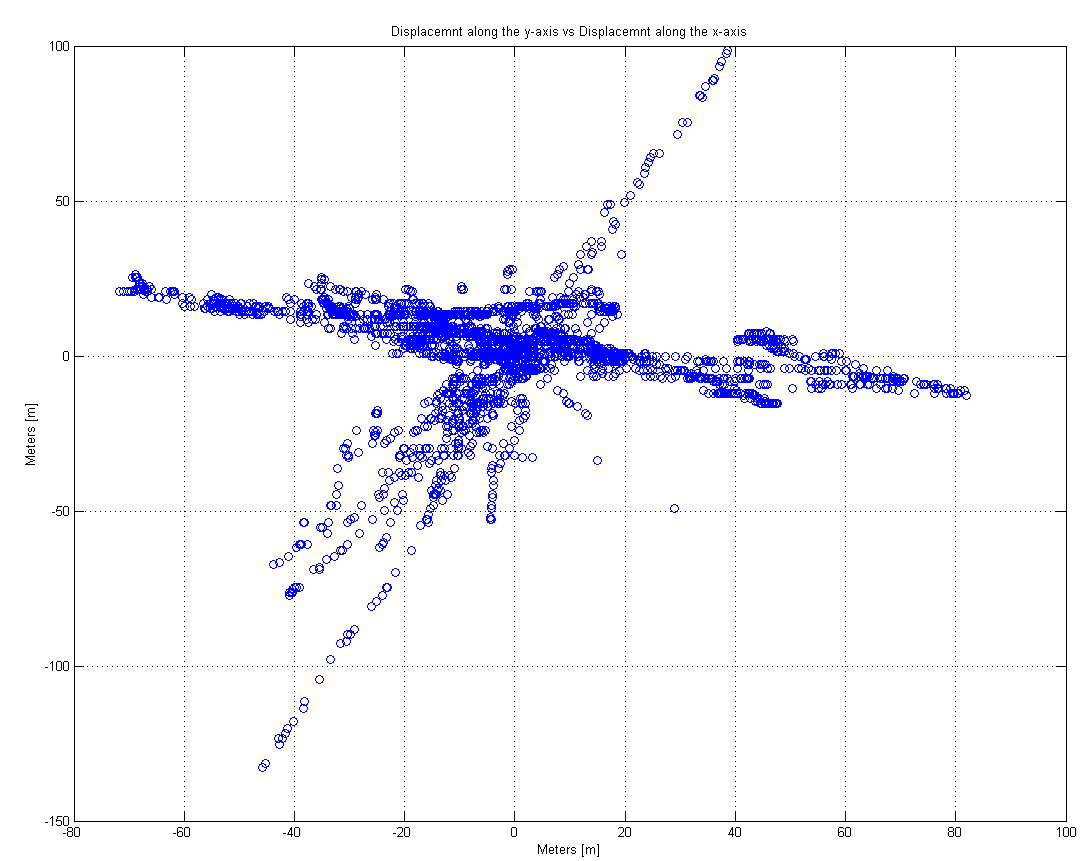
\includegraphics[width =0.7\paperwidth, height = 10cm]{\DocRoot/images/xy_plot_gps}
							\caption{Plot of \gls{gps} data in x-y plane}
							\label{Fig: Plot of gps data in x-y plane}
						\end{figure}

						\begin{figure}[h!]
							\centering
							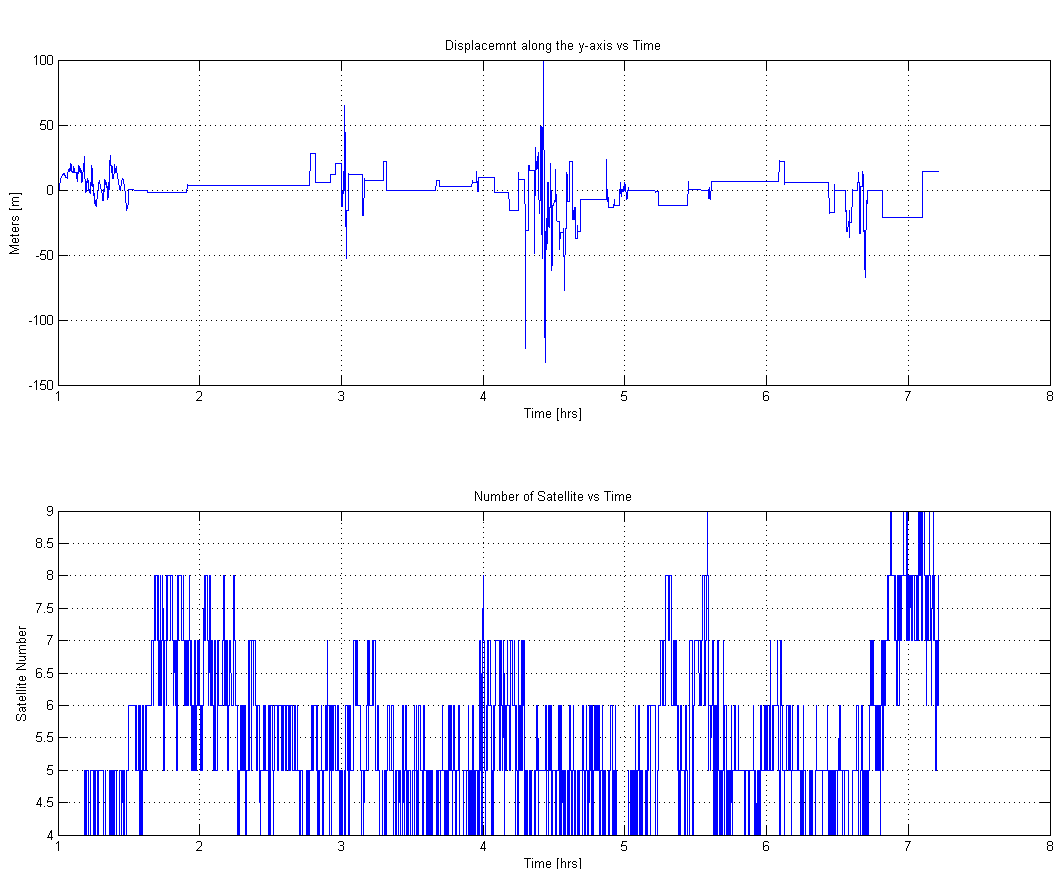
\includegraphics[width =0.5\paperwidth]{\DocRoot/images/x_plot_gps}
							\caption{Plot of \gls{gps} data in displacement in x direction vs time}
							\label{Fig: Plot of gps data in displacement in x direction vs time}
						\end{figure}

						\begin{figure}[h!]
							\centering
							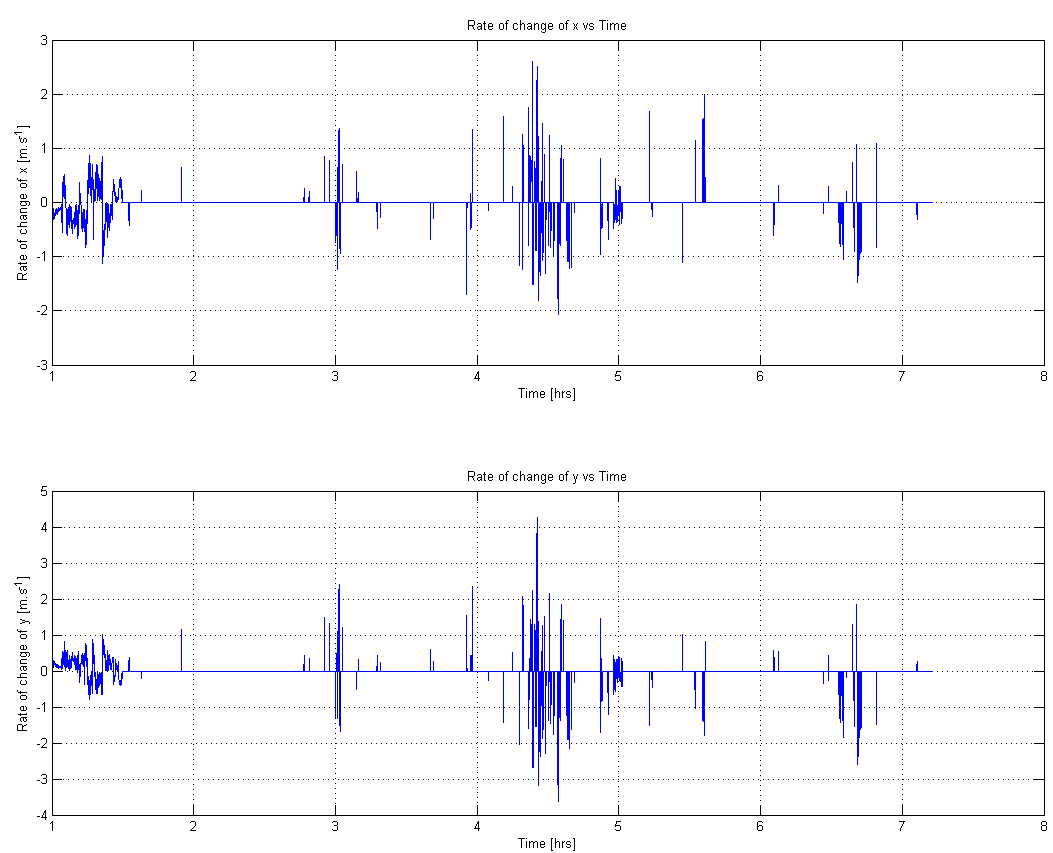
\includegraphics[width =0.5\paperwidth]{\DocRoot/images/x_rate_vs_time}
							\caption{Plot of \gls{gps} data in x rate vs time}
							\label{Fig: Plot of gps data in x rate vs time}
						\end{figure}


\newpage
 \tocless\section{Find the \gls{noisecomatrix} for the \gls{gps} Kalman Filter.}
From data collected the following \gls{noisecomatrix} where found for $x$ and $y$ respectively.
					\begin{equation}
					\gls{noisecomatrix}_{\gls{east}} = 		
					\left[\begin{array}{cc}
					\mathrm{cov(\gls{east})}       &                 0                          \\ 
					0                                                          & cov( \dot{x}_n   )          
					\end{array} \right]
					=					
					\left[\begin{array}{cc}
				 132.58    &                 0                          \\ 
					0                                                          & 0.0301         
					\end{array} \right]
					\end{equation}
					
										\begin{equation}
										\gls{noisecomatrix}_{\gls{north}} = 		
										\left[\begin{array}{cc}
										\mathrm{cov(\gls{north})}       &                 0                          \\ 
										0                                                          & cov( \dot{y}_n   )          
										\end{array} \right]
										=					
										\left[\begin{array}{cc}
										159.4762    &                 0                          \\ 
										0                                                          & 0.0617         
										\end{array} \right]
										\end{equation}
										
	 \tocless\section{\gls{gps} model used for Kalman Filter}			
	
	The $x$ model used by the kalman filter is defined as follows:-
						\begin{equation}
					\left[\begin{array}{c}
					\dot{\gls{east}}                          \\ 
					\ddot{\gls{east}}                                                          
					\end{array} \right] = 		
						\left[\begin{array}{cc}
					0       &                 1                         \\ 
						0                                                          &-\frac{ \gls{dampingx} }{\gls{systemmass}}        
						\end{array} \right]
				+
											\left[\begin{array}{c}
									      	0                         \\ 
											\frac{ 1 }{\gls{systemmass}}                                                       
											\end{array} \right] U					
						\end{equation}
and the $y$ modelled as follows.						
						\begin{equation}
						\left[\begin{array}{c}
						\dot{\gls{north}}                          \\ 
						\ddot{\gls{north}}                                                          
						\end{array} \right] = 		
						\left[\begin{array}{cc}
						0       &                 1                         \\ 
						0                                                          &-\frac{ \gls{dampingy} }{\gls{systemmass}}        
						\end{array} \right]
						+
						\left[\begin{array}{c}
						0                         \\ 
						\frac{ 1 }{\gls{systemmass}}                                                       
						\end{array} \right] U					
						\end{equation}
	
 \tocless\section{Test Quad-rotor}
Fixing issues with program run-time on Propeller and the quad-rotor was stabilised about the pitch and roll axis.						
%\chapter{Week 8: 9\textsuperscript{th} - 15\textsuperscript{th} March }
%\chapter{Week 9: 16\textsuperscript{th} - 22\textsuperscript{nd} March }
%\chapter{Week 10: 23\textsuperscript{rd} - 29\textsuperscript{th} March }
%\chapter{Week 11: 30\textsuperscript{th}  March  - 5\textsuperscript{th} April }
\chapter{ Complementary Filter}
A pair of filters are called complementary filters if their transfer functions sum to one at all frequencies in a complex sense, i.e. the phase is zero and the magnitude is one.






A complementary filter is easily derived by solving the transfer function of the Mahony \& Madgwick filter for the angle $\theta$, which yields

\begin{equation}
\theta = {\frac{1 + \frac{K_p}{K_i}s}{1 + \frac{K_p}{K_i}s + \frac{1}{K_i}s^2}}a + {\frac{\frac{1}{K_i}S^2}{1+\frac{K_p}{K_i}s + \frac{1}{K_i}s^2}\frac{1}{s}\omega}
\end{equation}

Obviously, and not unexpectedly, this complementary filter is build from $2^{\mathrm{nd}}$ order filters. Note that the filter acting on the acceleration data actually consists of a low-pass plus band-pass filter.

This result has interesting consequences. Being $2^{\mathrm{nd}}$ order filters, the frequency response of the acceleration and rotation rate filters are characterized by the resonance frequency and damping factor

\begin{equation}
\omega_0 = \sqrt{K_i}~~~~~~~ \xi = \frac{K_p}{2\sqrt{K_i}}
\end{equation}

The damping factor determines the overshoot at the resonance frequency. For high-pass (and low-pass) filters the frequency response is flat (and the step response non-oscillatory) for $\xi \geq 1$. This suggests the criterion \footnote{See \url{http://www.olliw.eu/2013/imu-data-fusing/} for more details}.

\begin{equation}
K_i \leq \frac{1}{4}K_p^2
\end{equation}
\end{document}